%----------------------------------------------------------------------
% Template for TECHNICAL REPORTS at Inst. of Computer Graphics
% and Vision (ICG), Graz University of Technology, Austria:
% style file 'techrep_icg.sty'
%
% author:  Pierre Elbischger
% email:   pierre.elibschger@icg.tu-graz.ac.at
%
% created: 13.11.2003
% revised: 29.04.2017 (Peter M. Roth, pmroth@icg.tugraz.at)
% revised: 15.09.2017 (Horst Possegger, possegger@icg.tugraz.at)
%----------------------------------------------------------------------
% The template contains a number of LaTeX commands of the form :
%
% \command{xyz}
%
% In order to complete this template, fill in the blank fields between
% the curly braces or replace already filled in fields with the
% requested information.
%
% e.g. in order to add a title, replace
% \title{} with \title{Evidence of Solitons in Tedium Diboride}
%
% The \author and \address commands can take an optional label
% in square brackets of the form :
%
% \command[label]{}
%
% The text of the abstract should be inserted between the two commands
% \begin{abstract} and \end{abstract}.
%
% Please leave all commands in place even if you don't fill them in.


%----------------------------------------------------------------------
% Do not alter the following two lines

\documentclass[11pt,a4paper]{article}
\usepackage{techrep_icg}

%----------------------------------------------------------------------
% Include any additional packages here!
% package 'graphicx' is automatically included depending on the
%   used compiler (latex, pdflatex), don't include it!!!

\usepackage{amsmath}
\usepackage{multirow}
\usepackage{subcaption}
\usepackage{url}
\usepackage{longtable}
\usepackage[inline]{enumitem}
%\usepackage{caption}
%\captionsetup[subfigure]{labelformat=empty}
\usepackage{makecell}
\captionsetup[subfigure]{font=normalsize,labelfont=normalsize}

\usepackage{booktabs}
\usepackage{pifont}

\usepackage{footnotebackref}

\newcommand*\rot{\rotatebox[origin=c]{90}}
\newcommand\RotText[1]{\rotatebox{90}{\parbox{3.5cm}{\centering#1}}}

\begin{document}
%----------------------------------------------------------------------
% Add the following information, which will be shown on the cover sheet

% Uncomment matching document type
% \type{Technical Report}
\type{Seminar/Project Computer Vision}
% \type{Seminar/Project Computer Graphics}
% \type{Master Project}
% \type{Bachelor Thesis}
% \type{Seminar Paper}


% Number of the technical report (if type == Technical Report)
\reportnr{xxx}

% Name of advisor (if type != Technical Report)
\advisor{Advisor: Dipl.-Ing. Erich Kobler}
\supervisor{Supervisor: Prof. Dr. Thomas Pock}

% Title
\title{Deep Restore}

% Subtitle
%\subtitle{This is the subtitle}
\subtitle{Using Image Segmentation and Image In-painting Techniques}

% City where the report was created
\repcity{Graz}

% Date of creation
\repdate{\today}

% Keywords that appear below the abstract (if required)
\keywords{Computer Vision, Film Restoration, Machine Learning, Image Segmentation, Image In-painting}

% List of authors: List each author using a separate \author{} command. If there 
% is more than one author address, add a label to each author of the form 
% \author[label]{name}. This label should be identical to the corresponding 
% label provided with the \address command. It is not possible to link an author 
% to more than one address!
%
\author[ICG]{Matthias Reiterer, BSc}


% List of addresses:  If there is more than one address, list each using a 
% separate \address command using a label to link it to the respective author
% as described above.
%
\newcommand{\TUGn}{Graz University of Technology}
\address[ICG]{Institute of Computer Graphics and Vision \\ \TUGn, Austria}


% Contact author: If \contact is not defined (uncommented) or empty, the contact  
% information on the title page is suppressed.
%
\contact{Matthias Reiterer, BSc}
\contactemail{matthias.reiterer@student.tugraz.at}

%----------------------------------------------------------------------
% Abstract:
\begin{abstract}
Analog movies, recorded on roll film, have the property that their image quality worsens statically either from usage or by time. To prevent this deterioration from happening, analog movies often get digitalized. The digitalization of analog movies has the advantage that during post-processing steps the image quality of previously analog movies can be improved - this is known as film restoration.\\

In this project, we will focus on such a post-processing step, namely the removing of impurities in single image frames. Based on previous research in the field of image restoration we came up with a step-wise solution: first, we detect the impurities of each image and generate a segmentation mask (image segmentation), and second, based on this segmentation mask we fill the impurities by using information from surrounding pixels (image in-painting).\\

Throughout this project, we mainly focus on modern machine learning approaches, especially convolutional neural networks (CNNs). For the image segmentation we test different architectures and regularization techniques to come up with a suitable architecture which gives the best results for the segmentation mask.\\

After we generated the segmentation mask we can perform image in-painting of the impure pixels. Again, we test different CNN-architectures and another method, image in-painting based on Perona-Malik-Diffusion.\\

We evaluate our approaches on ground truth data given from HS-Art~\cite{hs-art}. The results show that our method produces visually pleasing images.

\end{abstract}
%----------------------------------------------------------------------


%----------------------------------------------------------------------
% Main document 

{\tableofcontents}
\pagebreak

\section{Introduction}
\label{sec:num1}

"Deep Restore" - a combination of the two terms "deep learning" and "image restore". As the name of this project suggests, we focus our considerations on image restoration based on deep learning methods. This project is done in cooperation with HS-Art~\cite{hs-art}, who specialize in fields of archive film restoration and preservation\footnote{All the images used in this project are provided by HS-Art~\cite{hs-art}.}.


Image restoration describes the process of determining undistorted images from corrupted ones. It is used in a wide range of image and video processing applications and it is a basic method in computer vision. There exist many different approaches and an overview on some techniques can be found in Section~\ref{sec:num2}.

As Goodfellow et al.~\cite{Goodfellow16} state, deep learning is a part of machine learning methods based on feature learning and it is nowadays present in different fields like: computer vision, speech and audio recognition, bioinformatics and others. The learning of complicated tasks is based on the combination of many simpler ones and this hierarchy structure is deep, hence the name deep learning. There are different deep learning architectures like \textit{e.g.} recurrent neural networks (RNNs), Boltzmann machines, convolutional neural networks (CNNs), \textit{etc}. The learning of these architectures can either happen supervised, semi-supervised or unsupervised.

Since we focus on image restoration in this project, we decide to use CNNs to estimate undistorted images.  CNNs are feed-forward neural networks and are typically applied to inputs with local structure, \textit{i.e.} that consecutive and/or neighboring input features are more correlated than distant ones. Therefore, CNNs are mainly used in combination with images, video or audio. We choose to train our CNNs in a supervised manner. So, input images and ground-truth outputs combined are used to estimate the parameters of the networks.\\

As already mentioned, the goal of this project is to perform image restoration based on deep learning methods. Given a corrupted image (Figure~\ref{fig:intro_input}), we want to determine an undistorted image (Figure~\ref{fig:intro_restored}). 

\begin{figure}[H]
	\centering
	\begin{subfigure}{.3\textwidth}
		\centering
		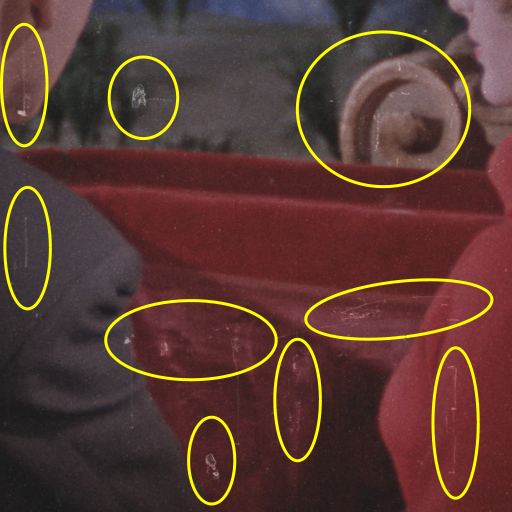
\includegraphics[width=\linewidth]{introduction/input.png}
		\caption[figure]{Impure image}
		\label{fig:intro_input}
	\end{subfigure}
	\begin{subfigure}{.3\textwidth}
		\centering
		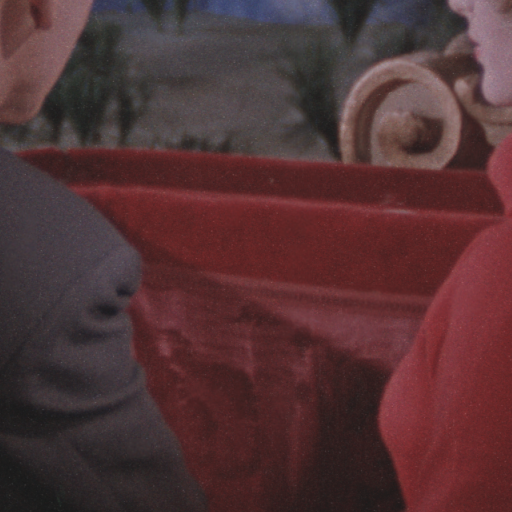
\includegraphics[width=\linewidth]{introduction/output.png}
		\caption[figure]{Restored image}
		\label{fig:intro_restored}
	\end{subfigure}
	\caption[figure]{An example of image restoration. (a) shows an image with impurities (yellow circled regions), whereas (b) shows an undistorted/restored variant of (a).}
	\label{fig:intro_desc}
\end{figure}

By investigating our given images and by performing research, we conclude that we can categorize the impurities of corrupted images into: \begin{enumerate*}[label=(\alph*)]\item dust, \item noise, other damages (like \item bent frames, \item scratches, \textit{etc.}) and for subsequent image frames \item flicker.\end{enumerate*} During this thesis we focus on: dust, noise and other damages. An overview of the different impurities is given in Figure~\ref{fig:impurities}, the images were taken from~\cite{hs-art2}.


\begin{table}[H]\begin{center}
\begin{tabular}{ c c c c }

 & \RotText{(a) Dust} & 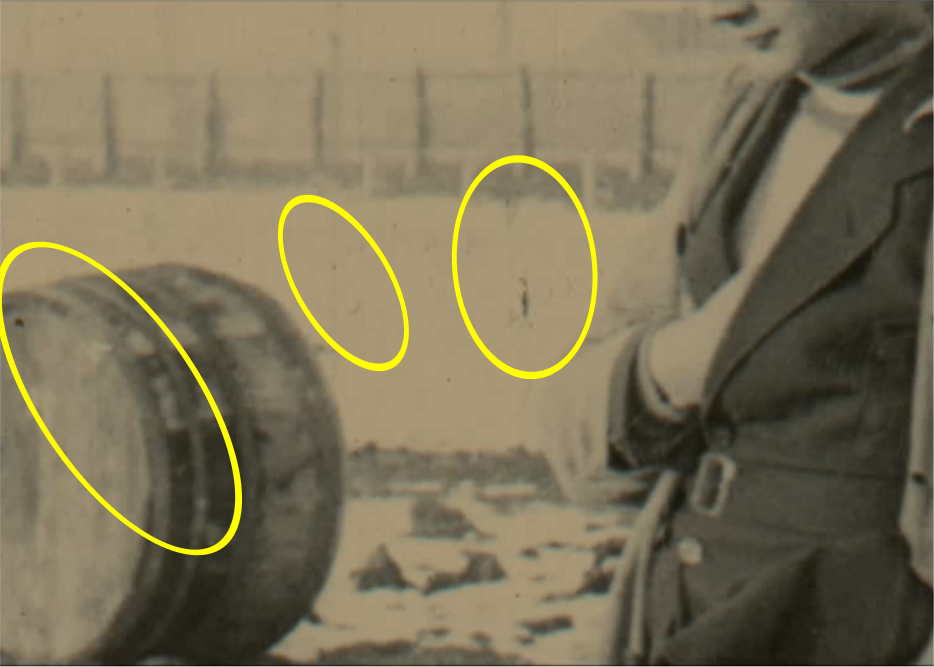
\includegraphics[width=.3\linewidth]{impurities/dust_1.png} & 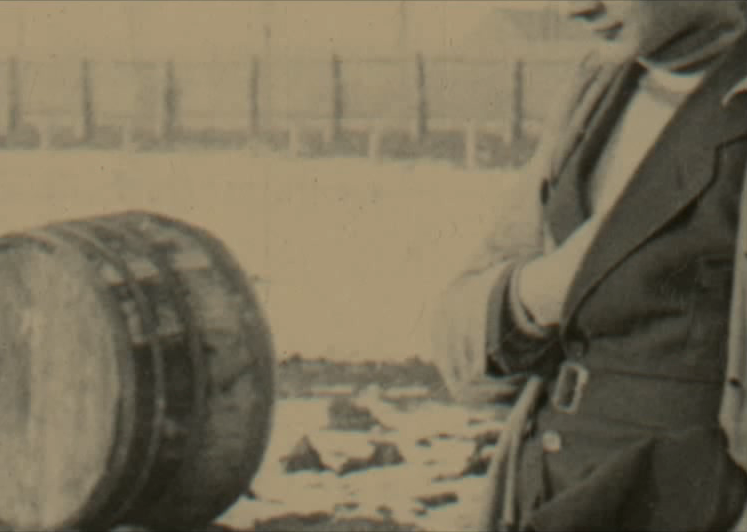
\includegraphics[width=.3\linewidth]{impurities/dust_2.png}\\
  
  & \RotText{(b) Noise} & 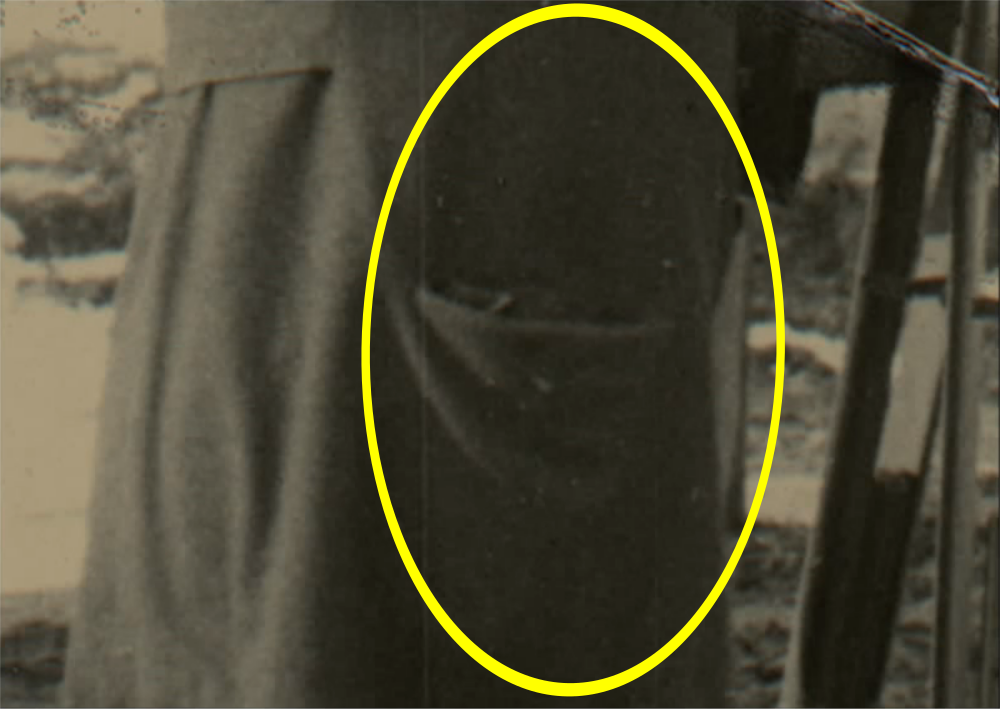
\includegraphics[width=.3\linewidth]{impurities/noise_1.png} & 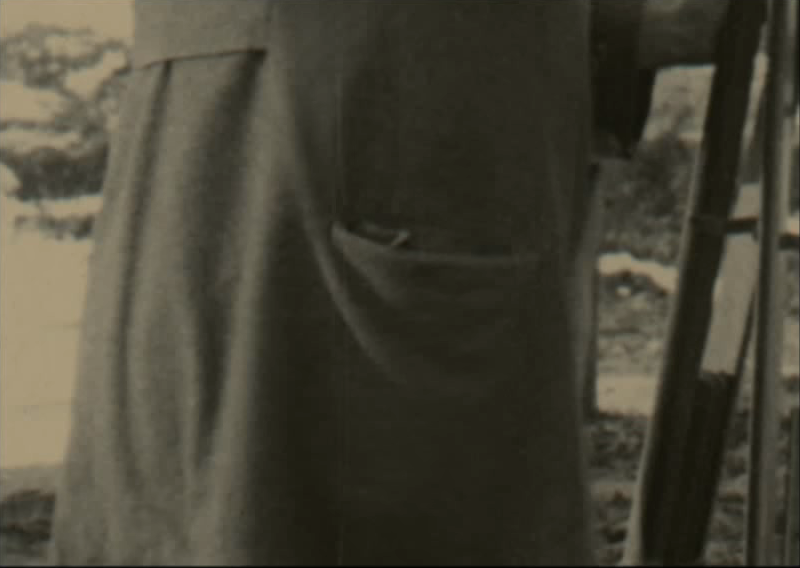
\includegraphics[width=.3\linewidth]{impurities/noise_2.png}\\
 
  & \RotText{(c) Scratch} & 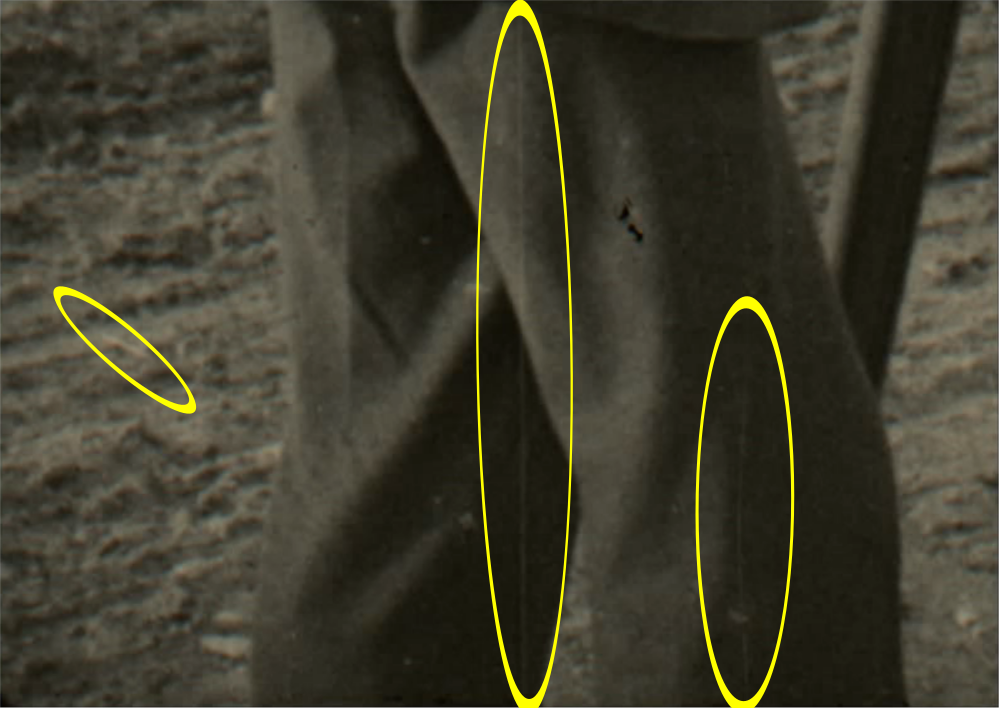
\includegraphics[width=.3\linewidth]{impurities/scratches_1.png} & 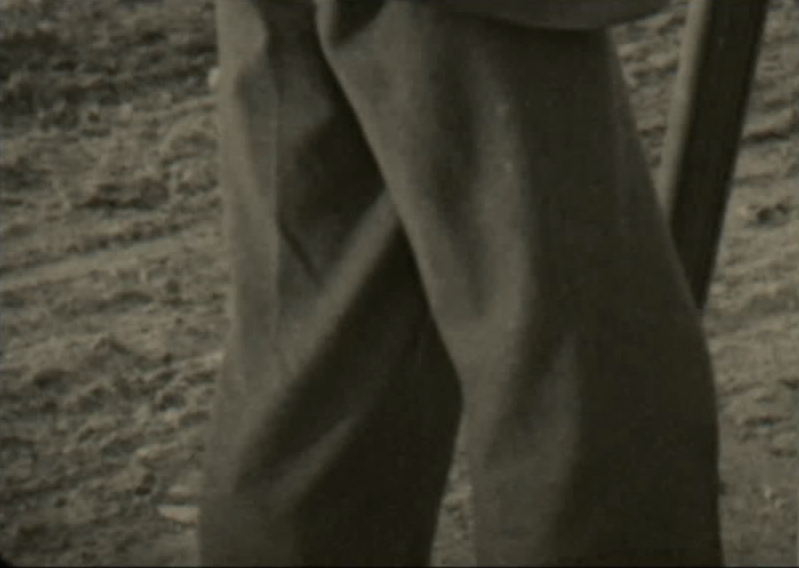
\includegraphics[width=.3\linewidth]{impurities/scratches_2.png}\\
   
  & \RotText{(d) Bent frame}&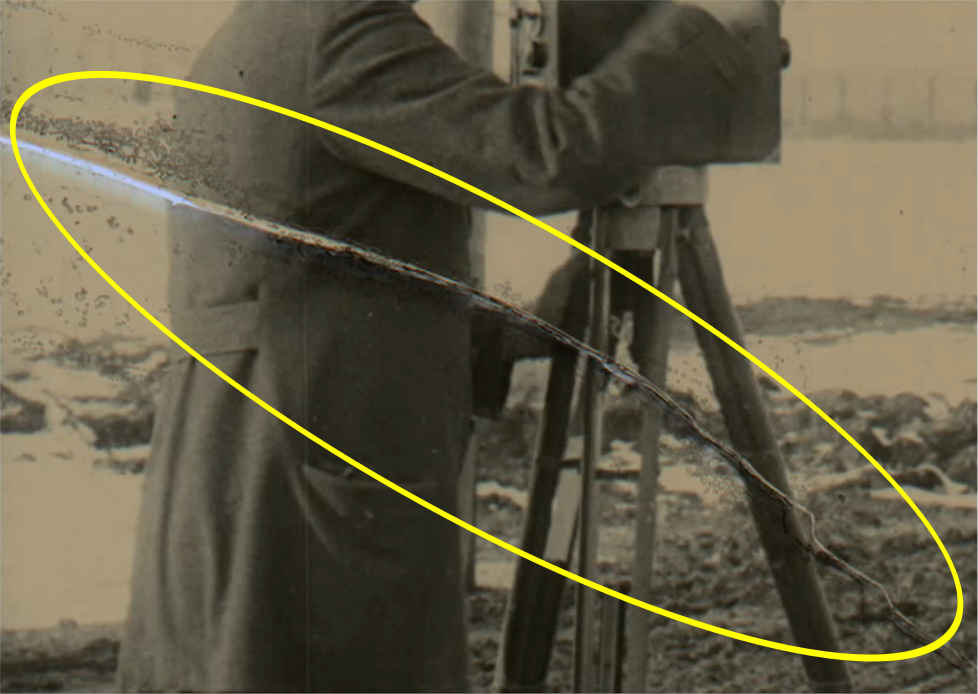
\includegraphics[width=.3\linewidth]{impurities/repairs_1.png} & 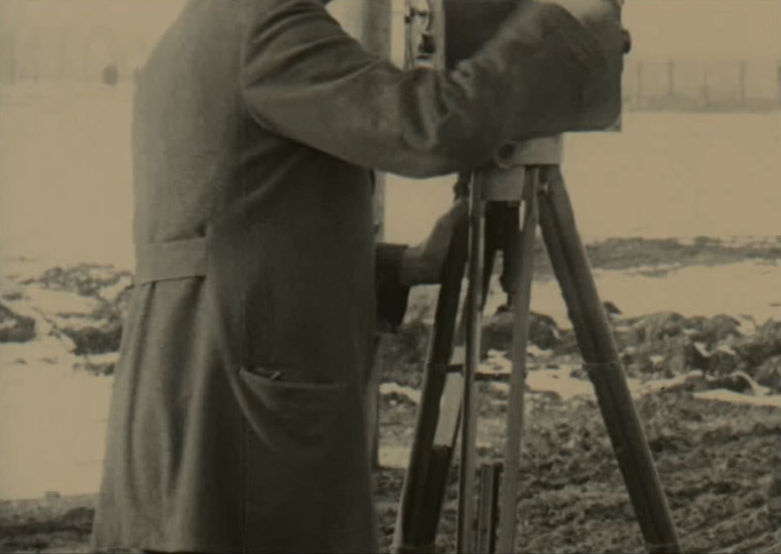
\includegraphics[width=.3\linewidth]{impurities/repairs_2.png} \\
   
   \parbox[t]{2mm}{\multirow{2}{*}{\rotatebox[origin=c]{90}{(e) Flicker}}} & \RotText{Frame 1} & 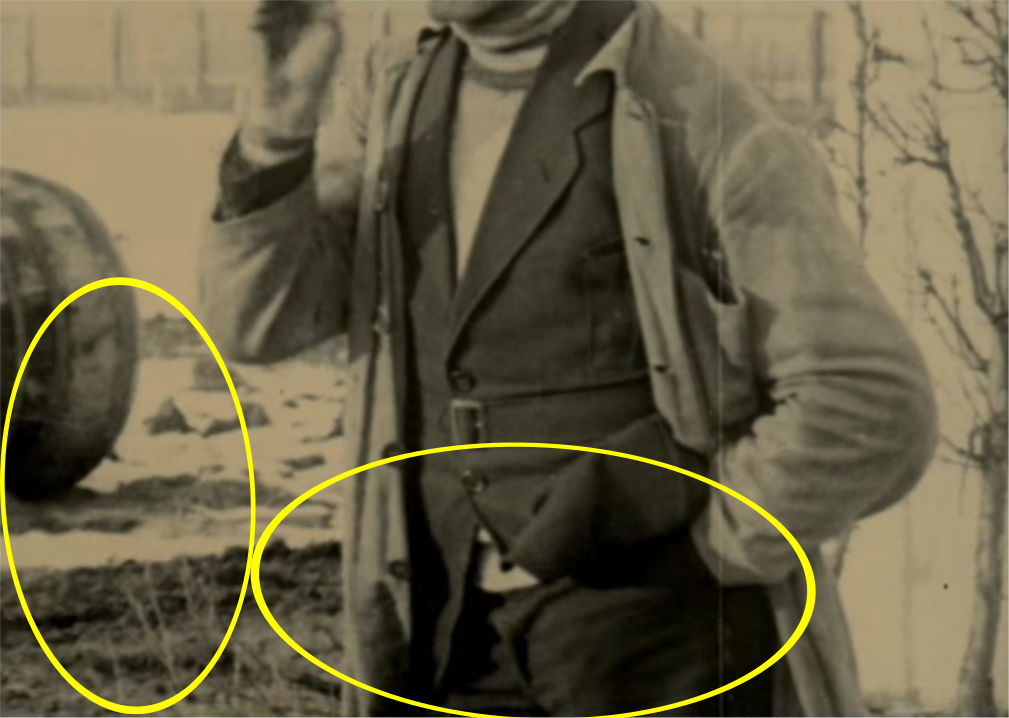
\includegraphics[width=.3\linewidth]{impurities/flicker1_1.png} & 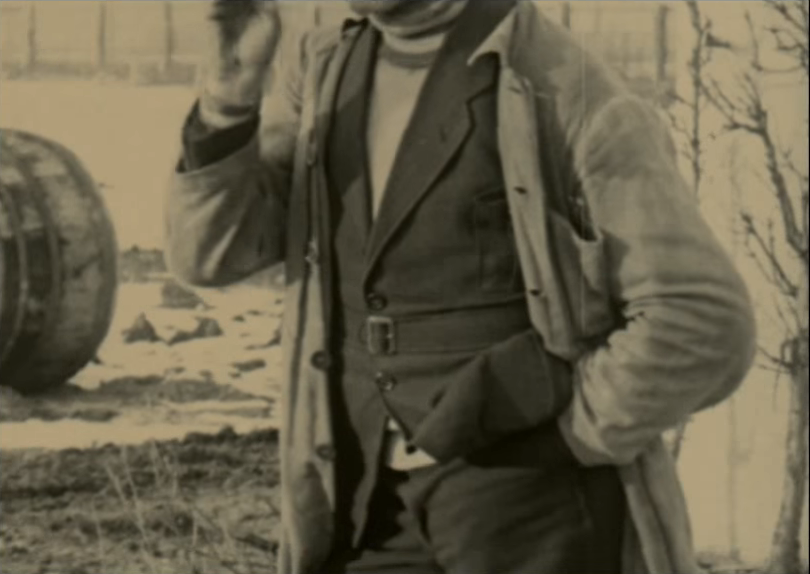
\includegraphics[width=.3\linewidth]{impurities/flicker1_2.png}\\
  
     & \RotText{Frame 2}&
     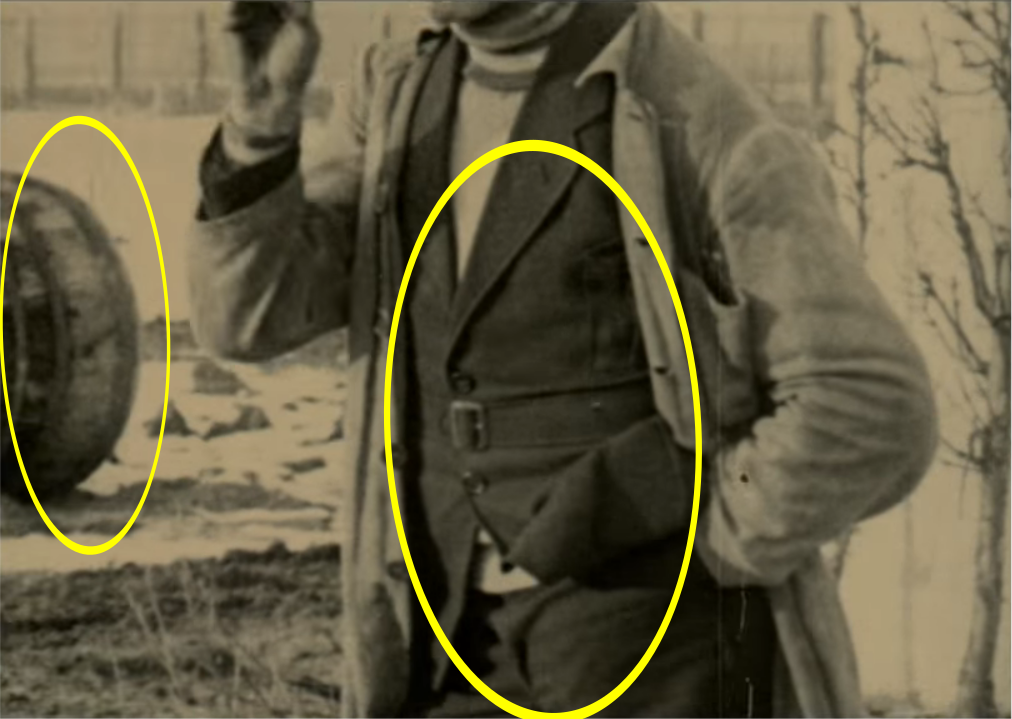
\includegraphics[width=.3\linewidth]{impurities/flicker2_1.png} & 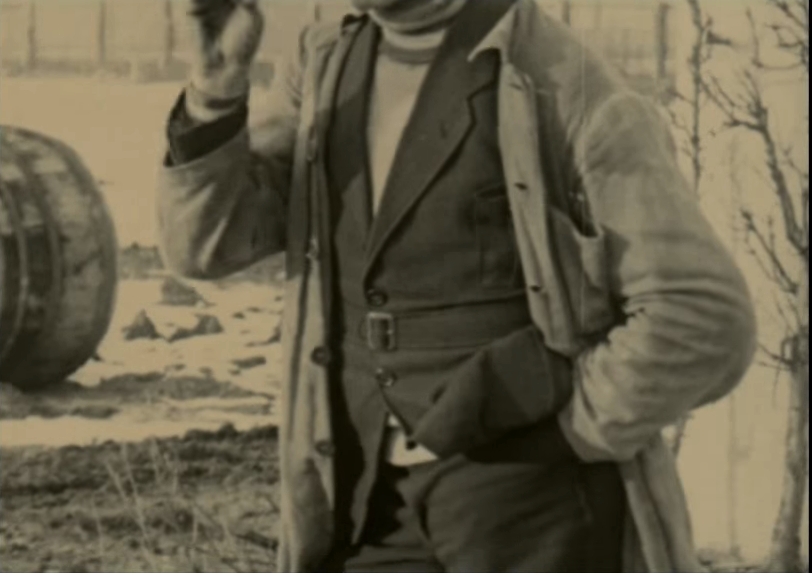
\includegraphics[width=.3\linewidth]{impurities/flicker2_2.png}\\
 & & Impure image & Restored image
\end{tabular}

\captionof{figure}{Different impurities and their restoration. For each of the different impurities (a) - (e) the corruption is highlighted in the left image (yellow circled regions) and the restored variant (right image) is shown.}

\label{fig:impurities}
\end{center}\end{table}


We split the workflow of image restoration into two consecutive steps: image segmentation and image in-painting. In the image segmentation step we generate a segmentation mask based on the input image. Image segmentation is the task of assigning a label to each pixel. In our case we have two labels, one label representing impurities and the other clear pixels. The resulting segmentation mask highlights impurities which are then removed. 

The next step is image in-painting. Image in-painting describes the process of filling in unknown pixels with information based on neighboring pixels. This is done by using the previously created segmentation mask and the input image. 

This worklow can be seen in Figure~\ref{fig:intro_flow}. In the first step we determine the segmantation mask (Figure~\ref{fig:intro_flow2}), where impurities are highlighted in white, from the input image (Figure~\ref{fig:intro_flow1}). Then, we perform image in-painting (Figure~\ref{fig:intro_flow3}) based on the segmentation mask (Figure~\ref{fig:intro_flow2}) and the input image (Figure~\ref{fig:intro_flow1}).




\begin{figure}[H]
	\centering
	\begin{subfigure}{.3\textwidth}
		\centering
		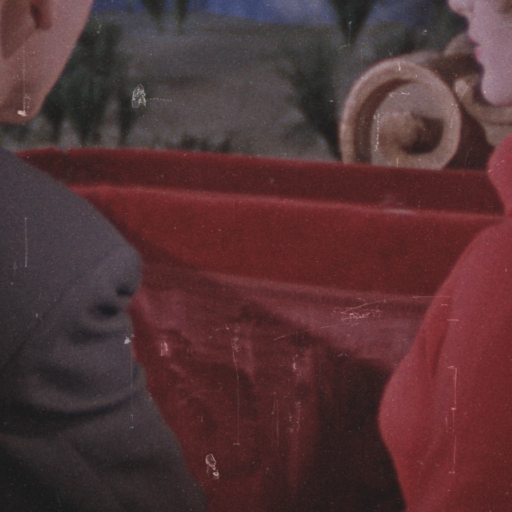
\includegraphics[width=\linewidth]{introduction/input_save.png}
		\caption[figure]{Input image}
		\label{fig:intro_flow1}
	\end{subfigure}
	\begin{subfigure}{.3\textwidth}
		\centering
		\setlength{\fboxrule}{0.5pt}
        \setlength{\fboxsep}{0pt}
        \framebox{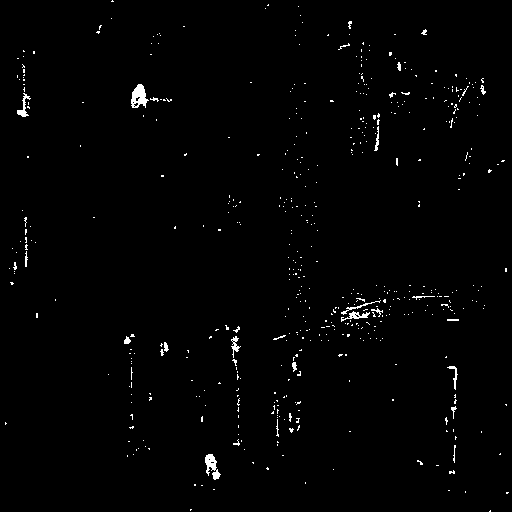
\includegraphics[width=\linewidth, decodearray={1 0 1 0 1 0}]{introduction/mask.png}}
		\caption[figure]{Generated mask}
		\label{fig:intro_flow2}
	\end{subfigure}
	\begin{subfigure}{.3\textwidth}
		\centering
		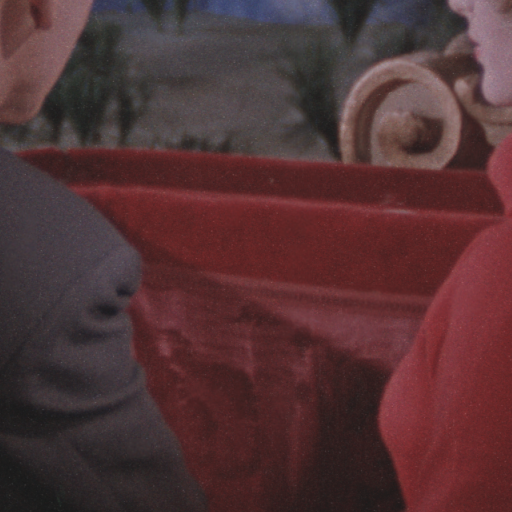
\includegraphics[width=\linewidth]{introduction/output.png}
		\caption[figure]{Restored image}
		\label{fig:intro_flow3}
	\end{subfigure}
	\caption[figure]{An example workflow of image restoration.}
	\label{fig:intro_flow}
\end{figure}


\section{Related Work}
\label{sec:num2}

Image restoration is a fundamental part of computer vision. There exist many different approaches and an overview on different techniques is given by Milanfar~\cite{Milanfar13}. Most of the current work on image restoration focuses on developing methods for achieving visual great looking results. This is mostly done by the cost of computational efficiency. Chen et al.~\cite{chen17} propose a method based on diffusion processes, which also takes computational efficiency into account.

Since we decided to split up the task of image restoration into image segmentation and image in-painting, the following Sections give an overview of different image segmentation techniques (Section~\ref{ssec:num21}) and image in-painting techniques (Section~\ref{ssec:num22}).


\subsection{Image Segmentation}
\label{ssec:num21}

Driven by a wide range of application, image segmentation received a significant amount of attention from the research community. Image segmentation is used in medical image processing for \textit{e.g.} segmenting cancer cells, in various object detection tasks, like pedestrian detection, video surveillance and others. 

Yuheng et al.~\cite{Yuheng17} categorize segmentation algorithms into: \begin{enumerate*}[label=(\roman*)] \item region-based threshold segmentation, \item regional growth segmentation, \item edge detection segmentation, \item segmentation based on clustering, and \item segmentation based on supervised learning with CNNs.\end{enumerate*} A newer approach from Qazanfari et al.~\cite{Qazanfari17} uses evolutionary computation that is inspired from human behavior to perform image segmentation.\\

We now focus on CNN based segmentation methods since this approach is most interesting for our project.  The recent usage of CNNs for various computer vision tasks but also image segmentation led in partly groundbreaking results. 

Long et al.\cite{long15} use fully convolutional networks to solve image segmentation. They adapt classification networks, such as VGG net~\cite{Simonyan14} or GoogLeNet~\cite{Szegedy15} into fully convolutional networks by transferring learned representations and combining semantic information from deep layers with appearance information from shallow layers.

In their work, Ronneberger et al.~\cite{Ronneberger15} propose a CNN architecture for image segmentation that consists of a contracting path to capture context and a symmetric expanding path that enables precise localization. This U-Net architecture achieves good performance on different biomedical segmentation tasks and is also used in other areas.
Huang et al.~\cite{Huang16} introduce in their work a dense convolutional network (DenseNet), in which each layer is connected to every other layer in a feed-forward fashion. Feature-maps of preceding layers are used as input for the current layer. An advantage of this architecture is that the number of parameter gets reduced.

The recent work of Chen et al.~\cite{Chen18} proposes new methods to further improve image segmentation with CNNs. They introduce convolution with upsampled filters to control the resolution at which feature responses are computed, a spatial pyramid pooling to segment object at multiple scales and to improve object localization, a combination of probabilistic  graphical models and CNNs.\\

During our project we take inspiration from the work of Huang et al.~\cite{Huang16} and Ronneberger et al.~\cite{Ronneberger15}.
 


\subsection{Image In-painting}
\label{ssec:num22}

Image in-painting is an ill-posed inverse problem with no well-defined solution. Its application reaches from removing text overlays or scratches, restoring lossy image transmission, object removal and others. 

Guillemot et al.~\cite{Guillemot2014} give an overview of different image in-painting techniques and categorizes as follows: \begin{enumerate*}[label=(\roman*)] \item in-painting using diffusion partial differential equations (PDEs), \item variational in-painting,  and \item examplar-based methods. Another category is \item image in-painting with the help of deep learning and machine learning. \end{enumerate*}

Diffusion based image in-painting, like the work of Boujena et al.~\cite{Boujena15}, rely heavily on the famous work of Perona~and~Malik~\cite{Perona90} and Weickert~\cite{weickert98}. Image diffusion is based on PDEs, where diffusion describes a physical process. The crucial part to establish a visual appealing in-painting, is to incorporate a diffusion tensor into the equations (a detailed description can be found in Section~\ref{ssec:num42}).
The work of Getreuer~\cite{getreuer12} and Neri et al.~\cite{Neri14} is based on total variation. The use slight variations of the total variation model for improved results. 

Related works in the machine learning sectors are \textit{e.g.} the work of Köhler et al.~\cite{Koehler14} and Gupta et al.~\cite{gupta17}. Köhler et al. use a CNN to perform image in-painting. They state that with an additional segmentation mask, highlighting missing pixels, the results of the in-painting can be improved. Gupta et al. use both CNN and RNN approaches.
Another recent trend in machine learning, that is popular in image in-painting, is the usage of an encoder-decoder structure or Generative adversarial network (GANs). Burlin et al.~\cite{burlin17}, Yeh et al.~\cite{Yeh17} and van Noord et al.~\cite{vanNoord18} all use this structure to perform state-of-the-art image in-painting.




\section{Image Segmentation}
\label{sec:num3}

In this Section follows a description of our methods and approaches for detecting impurities by image segmentation. As already mentioned, we focus on a machine learning approach namely CNNs. Section~\ref{ssec:num31} gives an overview of architectures that use just the current image to perform the image segmentation. Section~\ref{ssec:num32} shows architectures that use additional information, the previous and next image, to perform image segmentation of the current image. And Section~\ref{ssec:num32} lists the approach of using additional warped instances of the previous and next image.

It should be mentioned that if not stated otherwise, we use ReLU activation functions between layers and a sigmoid output activation function to perform image segmentation, which is in general a classification task.  We also apply regularization techniques that are described in Section~\ref{ssec:num34}. We choose the cross-entropy-error (CEE) for computing the loss/error between predicted and ground-truth segmentation masks.


\subsection{Single Input Image}
\label{ssec:num31}

Our first approach is to train simple architectures with few parameters to perform image segmentation (workflow: from Figure~\ref{fig:intro_flow1} to Figure~\ref{fig:intro_flow2}). We train all following networks on pairs of: single~images~+~ground-truth~masks. The different networks (Figure~\ref{fig:single_architecutes}) are: \begin{enumerate*}[label=(\alph*)]\item a simple one, consisting of five blocks, \item a network based on the work of Ronneberger et al.~\cite{Ronneberger15}, consisting of three layers and that uses a combination of max-pooling and de-convolution, and \item a network based on the work of Huang et al.~\cite{Huang16} that consists of five sub-blocks.\end{enumerate*}
The results of the different architectures are listed in Section~\ref{ssec:num531}.

\begin{figure}[H]
	\centering
	\begin{subfigure}{.70\textwidth}
		\centering
		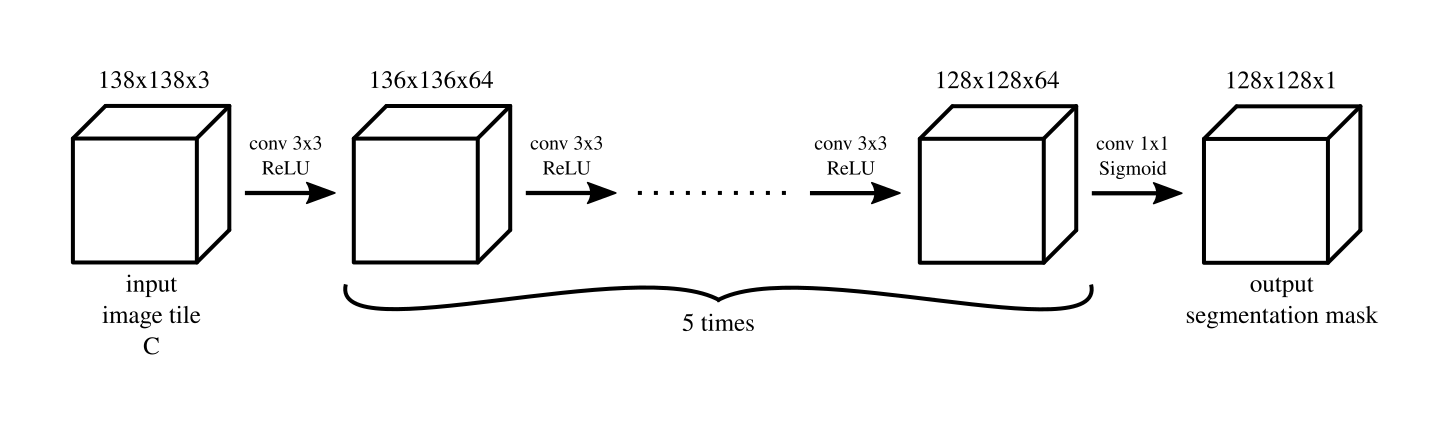
\includegraphics[width=\linewidth]{models_single/early.png}
		\caption[figure]{A "simple"-network with five blocks. An additional padding of size 5 was added to each $128\times128$ patch because valid-convolution was used.}
		\label{fig:single_simple}
	\end{subfigure}
\end{figure}
\begin{figure}[H]
  \ContinuedFloat
  \centering
		\begin{subfigure}{.95\textwidth}
		\centering
		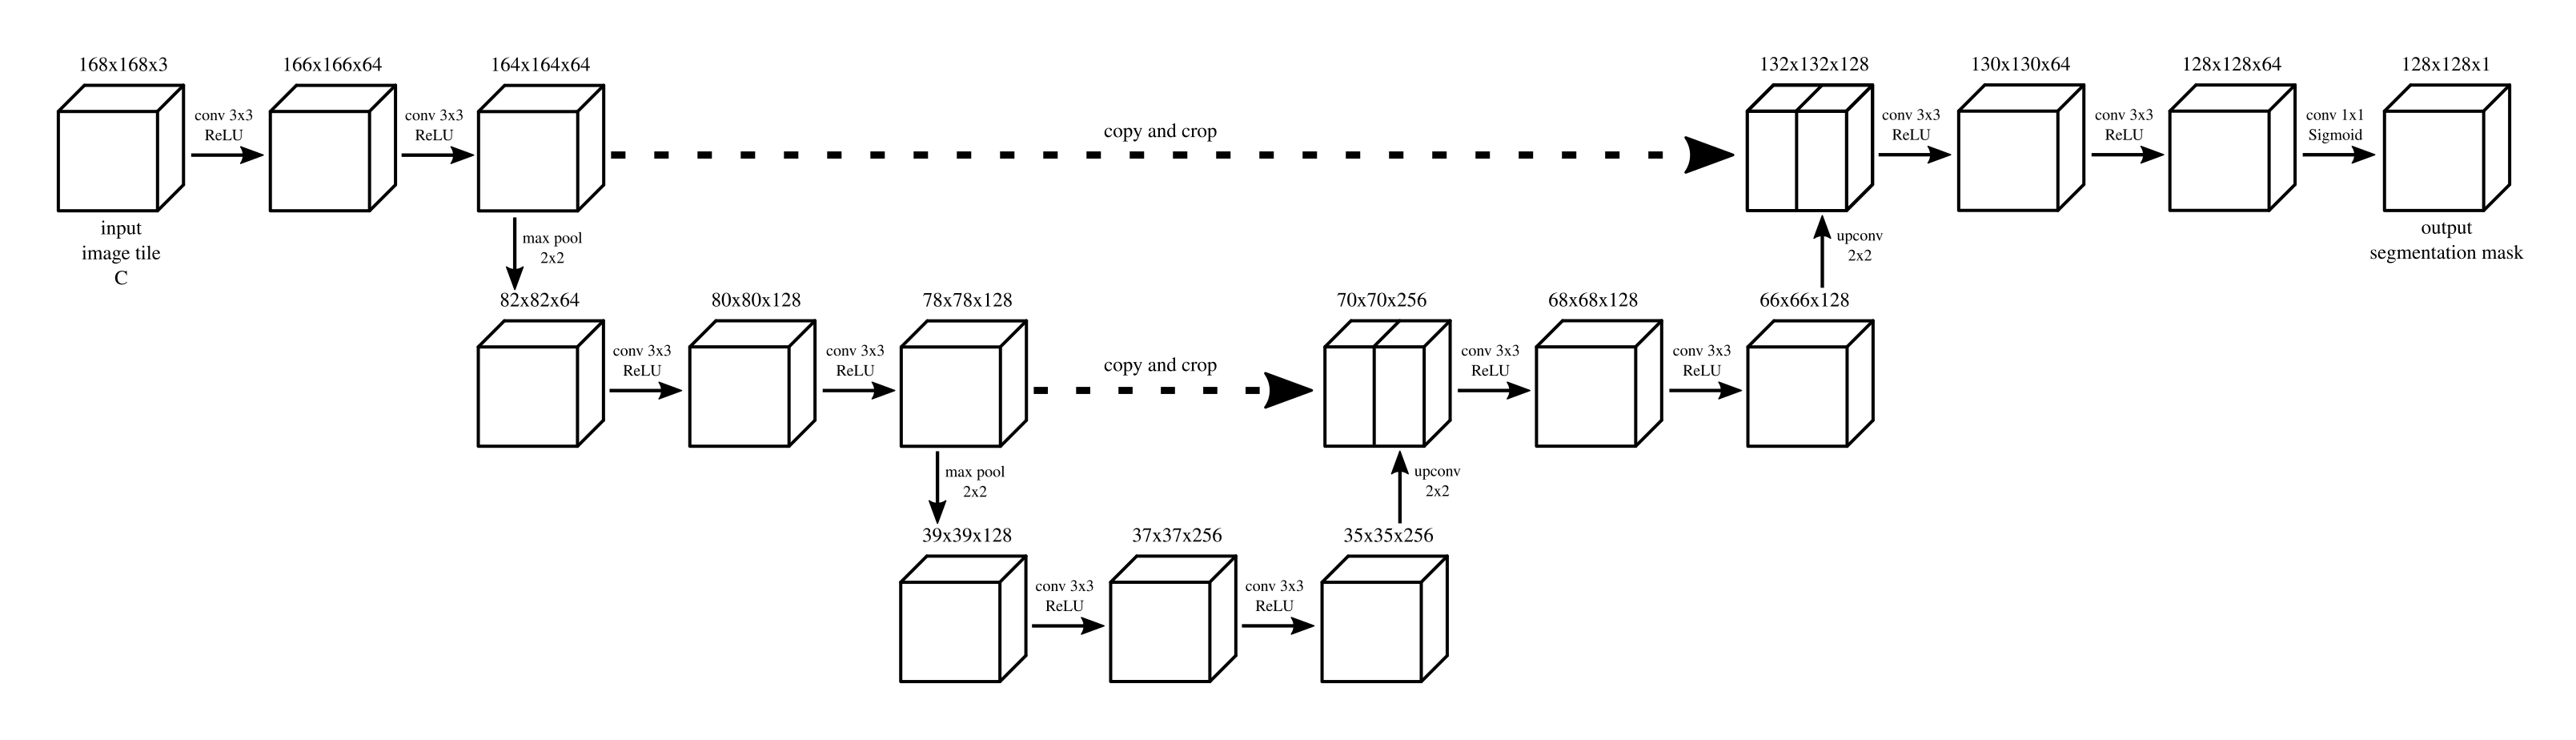
\includegraphics[width=\linewidth]{models_single/unet.png}
		\caption[figure]{An U-Net-network with three layers. An additional padding of size 15 was added to each $128\times128$ patch because valid convolution was used.}
		\label{fig:single_unet}
	\end{subfigure}
\end{figure}
\begin{figure}[H]
  \ContinuedFloat
  \centering
		\begin{subfigure}{.95\textwidth}
		\centering
		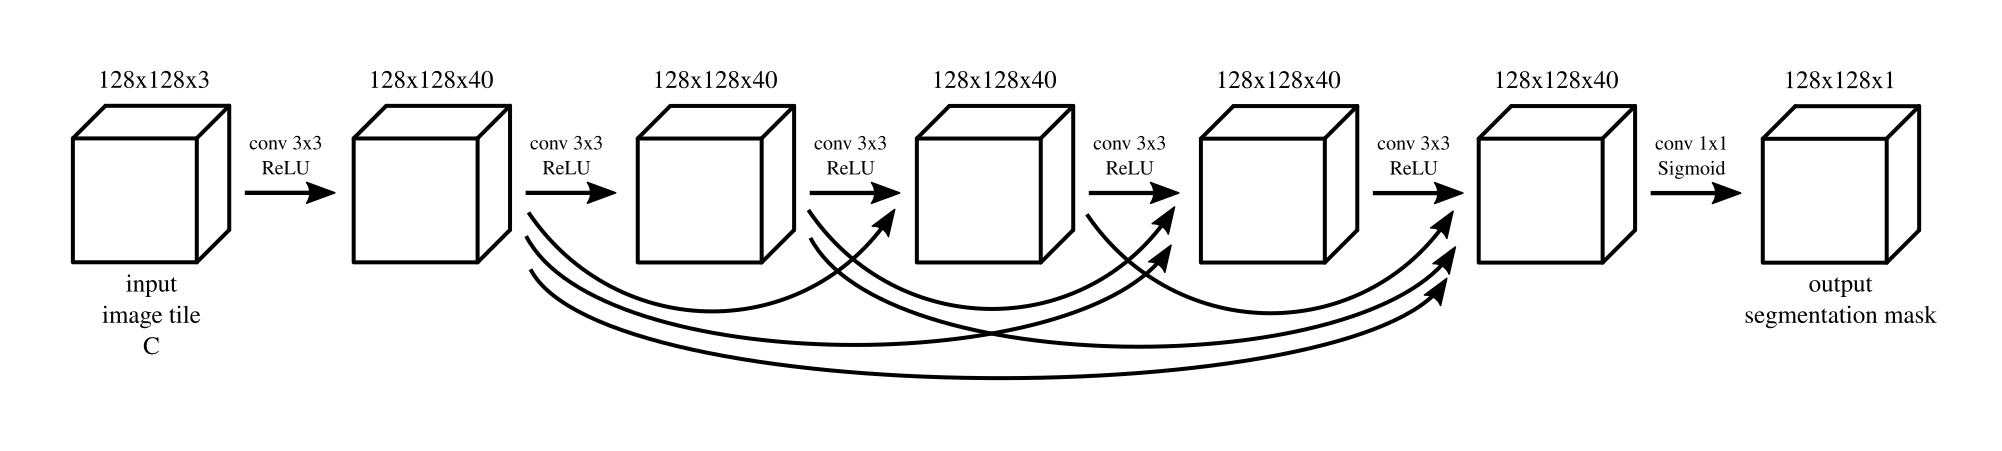
\includegraphics[width=\linewidth]{models_single/densenet.png}
		\caption[figure]{A densenet-network with five sub-blocks, this is later referred to as a single densenet block.}
		\label{fig:single_densenet}
	\end{subfigure}
	
	
	\caption[figure]{Different CNN architectures for image segmentation. The "C" in each Figure~(a)~-~(c), in "image tile C", stands for current and means that we just use information from the current image.}
	\label{fig:single_architecutes}
\end{figure}
Using just a single input image we achieved bad results (see Section~\ref{ssec:num531}). Thus, we decided to add additional information to our input, see Section~\ref{ssec:num32}.

\subsection{Multiple Input Images}
\label{ssec:num32}


This Section gives an overview of architectures that use additional input information to perform image segmentation (workflow: from Figure~\ref{fig:flow_input} and Figure~\ref{fig:flow_mask} to Figure~\ref{fig:flow_output}). We now also use the previous and next image to perform image segmentation on the current frame, see Figure~\ref{fig:flow_input}. In Figure~\ref{fig:flow_input} we can also see that impurities of the current frame (Figure~\ref{fig:flow_flow2}) are mostly not visible in the previous (Figure~\ref{fig:flow_flow1}) and next frame (Figure~\ref{fig:flow_flow3}). 


\begin{figure}[H]
	\centering
	\begin{subfigure}{.3\textwidth}
		\centering
		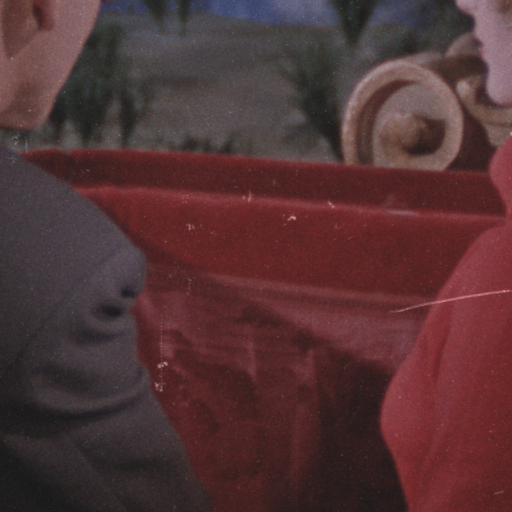
\includegraphics[width=\linewidth]{introduction/previous.png}
		\caption[figure]{Previous image}
		\label{fig:flow_flow1}
	\end{subfigure}
	\begin{subfigure}{.3\textwidth}
		\centering
		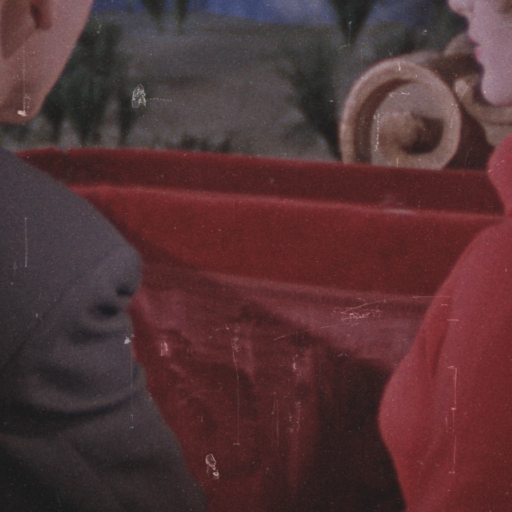
\includegraphics[width=\linewidth]{introduction/input_save.png}
		\caption[figure]{Input image}
		\label{fig:flow_flow2}
	\end{subfigure}
	\begin{subfigure}{.3\textwidth}
		\centering
		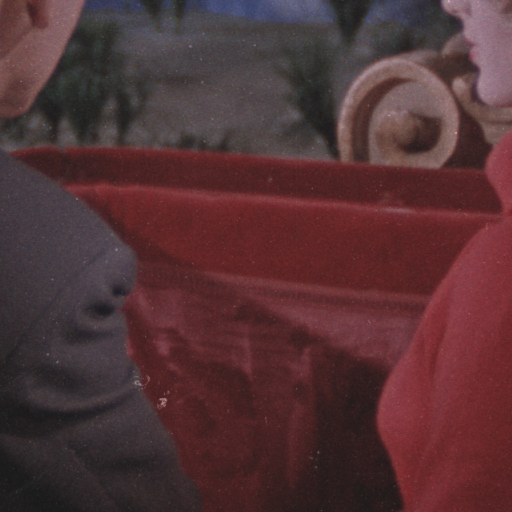
\includegraphics[width=\linewidth]{introduction/next.png}
		\caption[figure]{Next image}
		\label{fig:flow_flow3}
	\end{subfigure}
	\caption[figure]{An example of using additional information for image restoration by the usage of previous~(a), current input~(b) and next image~(c).}
	\label{fig:flow_input}
\end{figure}
	
\begin{figure}[H]
	\centering
	\begin{subfigure}{.3\textwidth}
		\centering
		\setlength{\fboxrule}{0.5pt}
        \setlength{\fboxsep}{0pt}
        \framebox{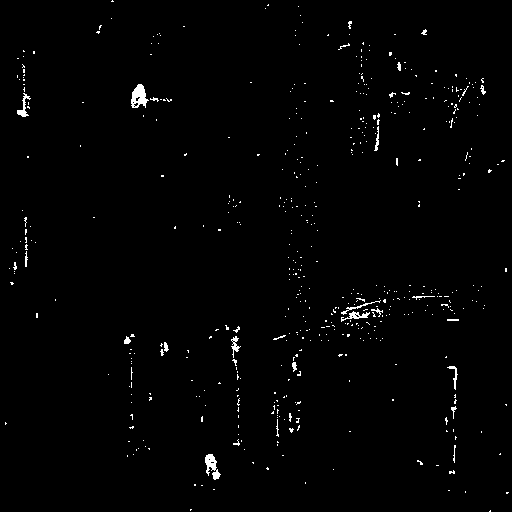
\includegraphics[width=\linewidth, decodearray={1 0 1 0 1 0}]{introduction/mask.png}}
		\caption[figure]{Generated mask}
		\label{fig:flow_mask}
	\end{subfigure}
	\begin{subfigure}{.3\textwidth}
		\centering
		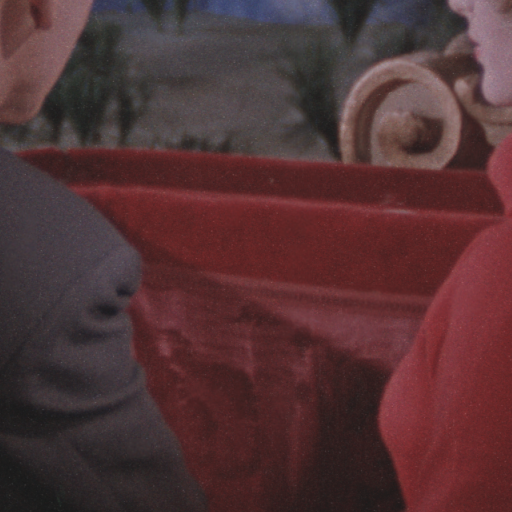
\includegraphics[width=\linewidth]{introduction/output.png}
		\caption[figure]{Output image}
		\label{fig:flow_output}
	\end{subfigure}
	\caption[figure]{An example workflow of image restoration using additional information (previous, current and next image, \textit{e.g.} Figure~\ref{fig:flow_input}) for generating the segmentation mask~(\ref{fig:flow_mask}) and in-painting~(\ref{fig:flow_output}).}
	\label{fig:flow_flow}
\end{figure}


The different networks (Figure~\ref{fig:flow_architecutes}) tested are: \begin{enumerate*}[label=(\alph*)]\item an early combine network consisting of five blocks. We name this network "early combine" since we combine the information of all images in the beginning. \item A late combine network that consists of two shared blocks (the line with the filled circle in Figure~\ref{fig:flow_late_combine}~and~\ref{fig:flow_densenet_comb} means that weights and biases are shared for this block). We name this network "late combine" since we combine the information of all images later. \item A network based on the work of Ronneberger et al.~\cite{Ronneberger15}, consisting of three layers and that uses a combination of max-pooling and de-convolution. \item A network based on the work of Huang et al.~\cite{Huang16} that consists of five sub-blocks. \item A network, again based on the work of Huang et al.~\cite{Huang16}, that consists of an upper path and a lower path. The upper path consists of two densenet blocks and the lower path of two shared densenet blocks. We combine the two paths via concatenating to achieve a final segmentation mask. The idea behind this concept is that the upper and lower path may learn different features that combined achieve better results. \item A bottleneck network consisting of five blocks. We name this network "bottleneck" because of its structure to reduce the features via a $1\times1$ convolution. This is done to reduce the parameters of the network. And, \item a network based on the work of Huang et al.~\cite{Huang16} and Ronneberger et al.~\cite{Ronneberger15}. It consists of an upper path and a lower path. The upper path consists of two densenet blocks and the lower path of an U-Net block with three layers. We subtract the intermediate results of the two paths to achieve a final segmentation mask. The idea behind this concept is the same as for the "densenet combine"-network (e). \end{enumerate*}
The results of the different architectures are listed in Section~\ref{ssec:num532}.

\begin{figure}[H]
	\centering
	\begin{subfigure}{.70\textwidth}
		\centering
		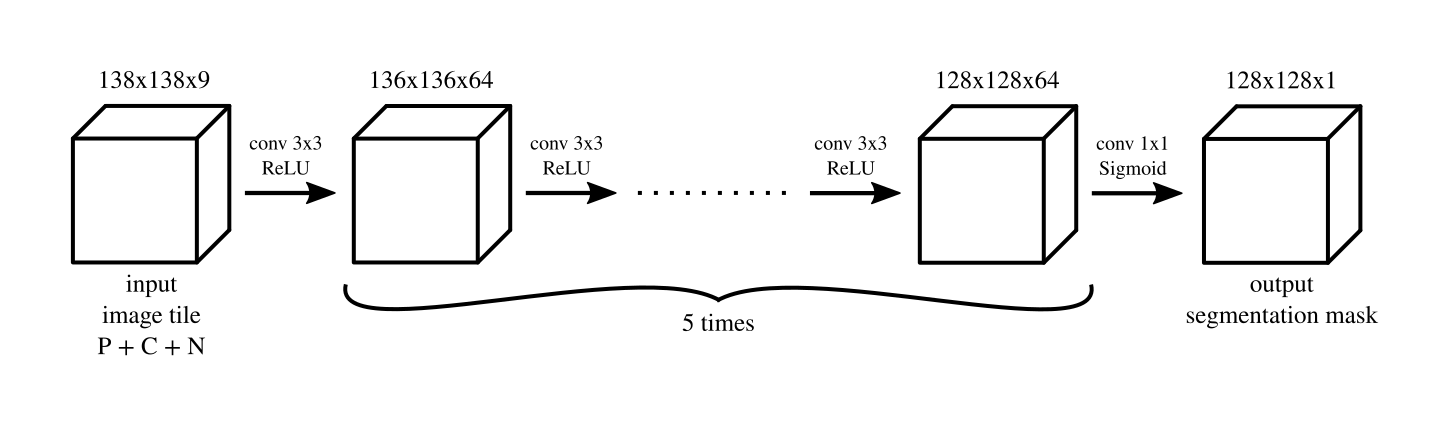
\includegraphics[width=\linewidth]{models_flow/early_combine.png}
		\caption[figure]{A "simple"-network with five blocks. An additional padding of size 5 was added to each $128\times128$ patch because valid-convolution was used.}
		\label{fig:flow_early_combine}
	\end{subfigure}
\end{figure}
\begin{figure}[H]
  \ContinuedFloat
  \centering	
	\begin{subfigure}{.95\textwidth}
		\centering
	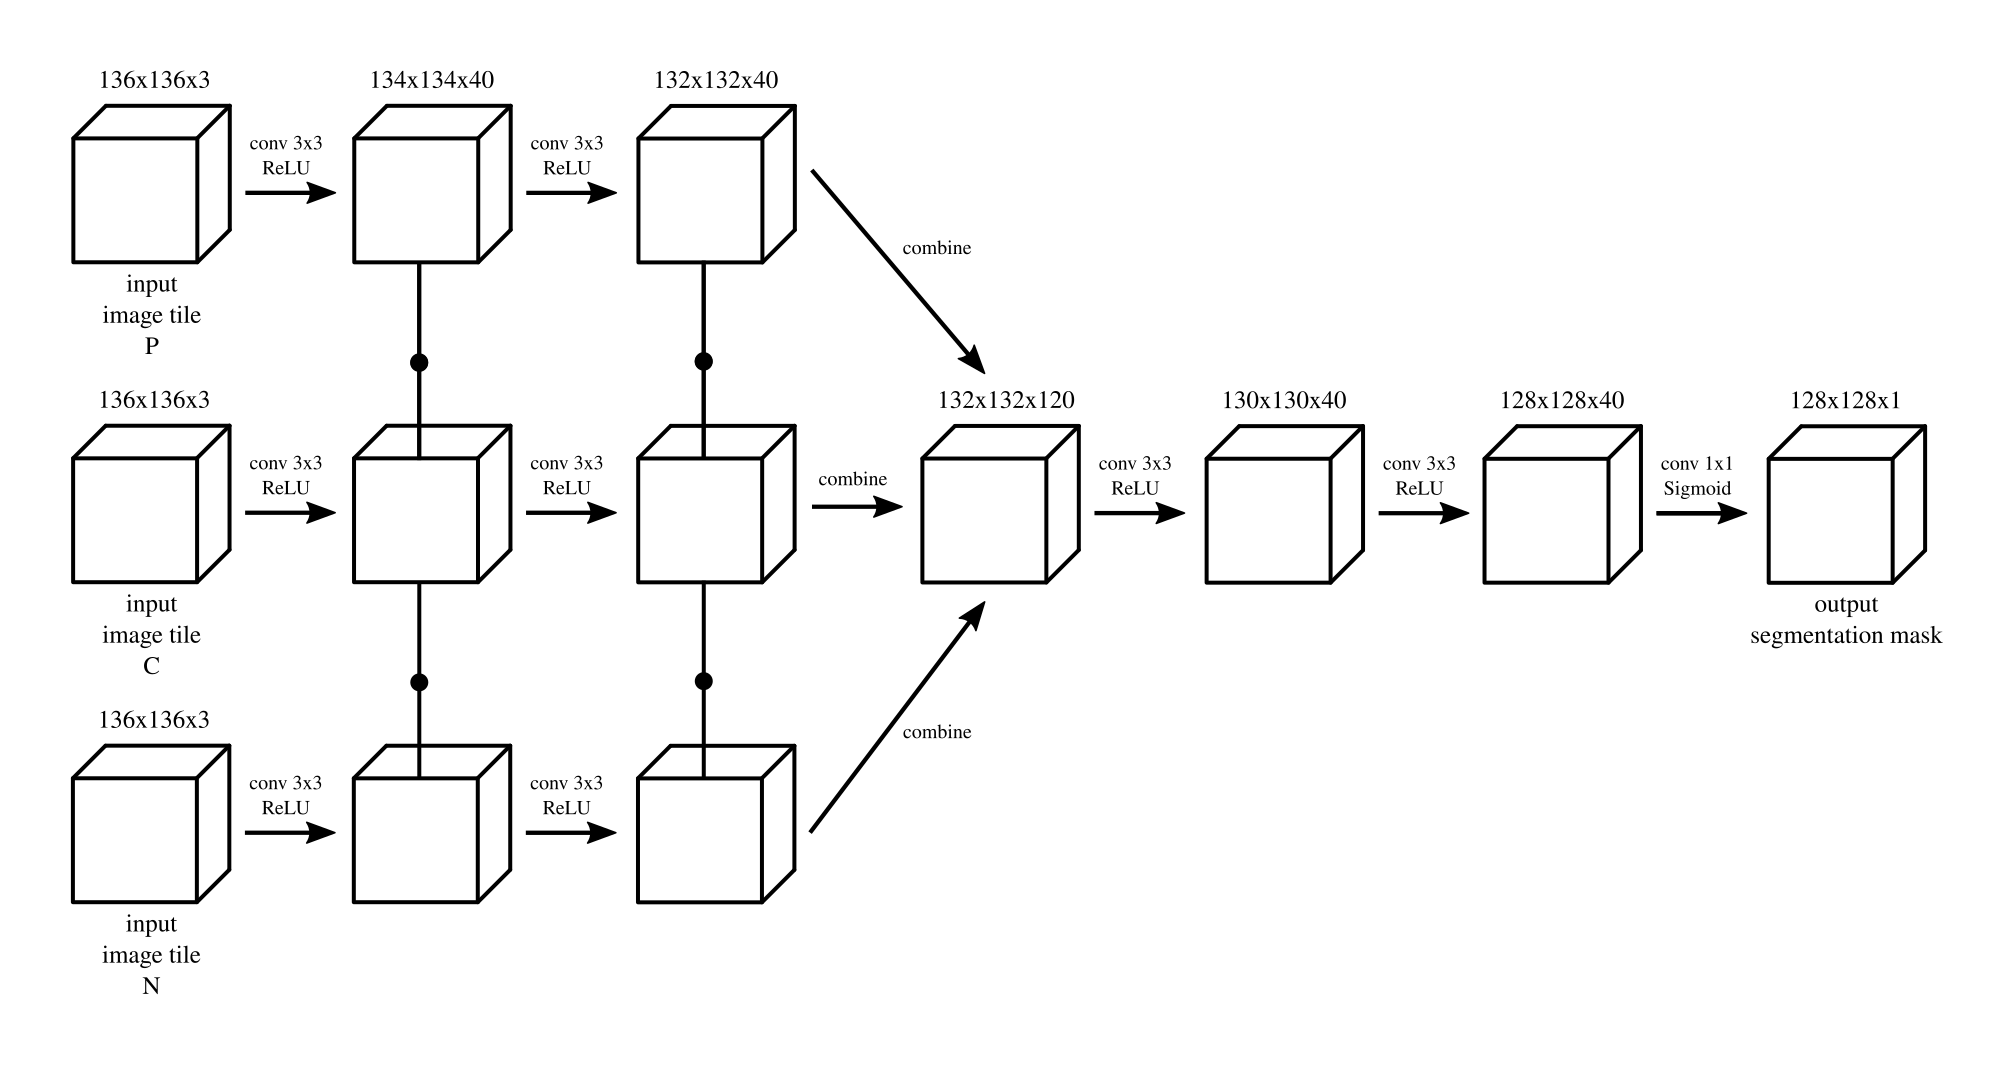
\includegraphics[width=\linewidth]{models_flow/late_combine.png}
	\caption[figure]{A "late combine"-network with two shared blocks. An additional padding of size 4 was added to each $128\times128$ patch because-valid convolution was used.}
	\label{fig:flow_late_combine}
	\end{subfigure}
\end{figure}
\begin{figure}[H]
  \ContinuedFloat
  \centering	
		\begin{subfigure}{.95\textwidth}
		\centering
		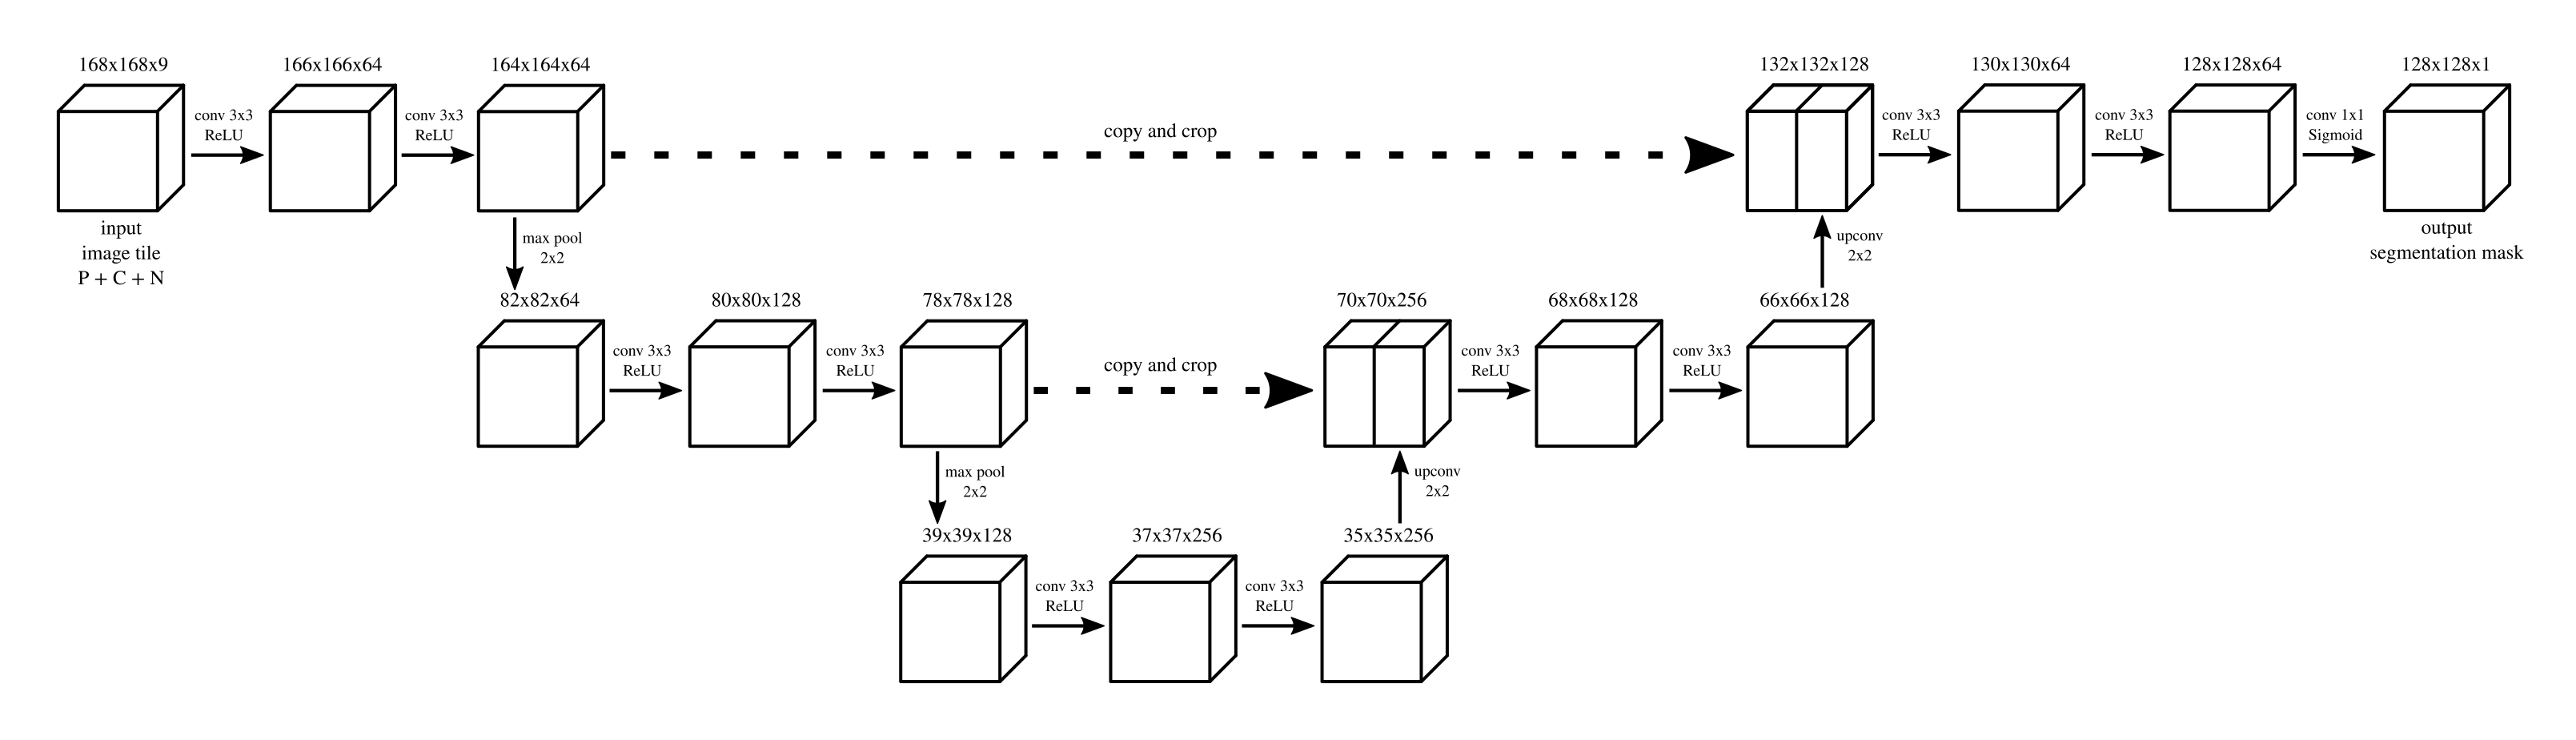
\includegraphics[width=\linewidth]{models_flow/unet.png}
	\caption[figure]{An U-Net-network with three layers. An additional padding of size 15 was added to each $128\times128$ patch because valid convolution was used.}
	
	\label{fig:flow_unet}
	\end{subfigure}
		\end{figure}
	\begin{figure}[H]
  \ContinuedFloat
  \centering
		\begin{subfigure}{.95\textwidth}
		\centering
		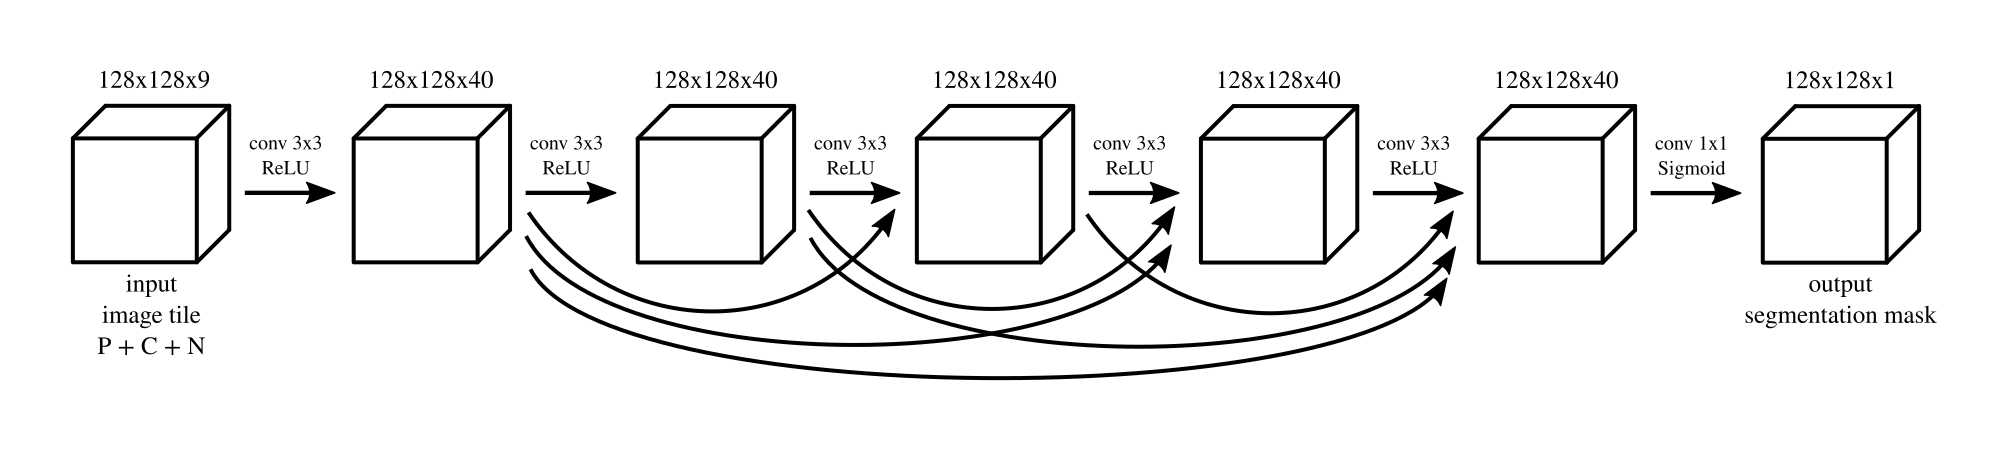
\includegraphics[width=\linewidth]{models_flow/densenet.png}
	\caption[figure]{A densenet-network with five sub-blocks, this is later referred to as a single densenet block.}
	\label{fig:flow_densenet}
	\end{subfigure}
\end{figure}
\begin{figure}[H]
  \ContinuedFloat
  \centering
			\begin{subfigure}{.95\textwidth}
		\centering
		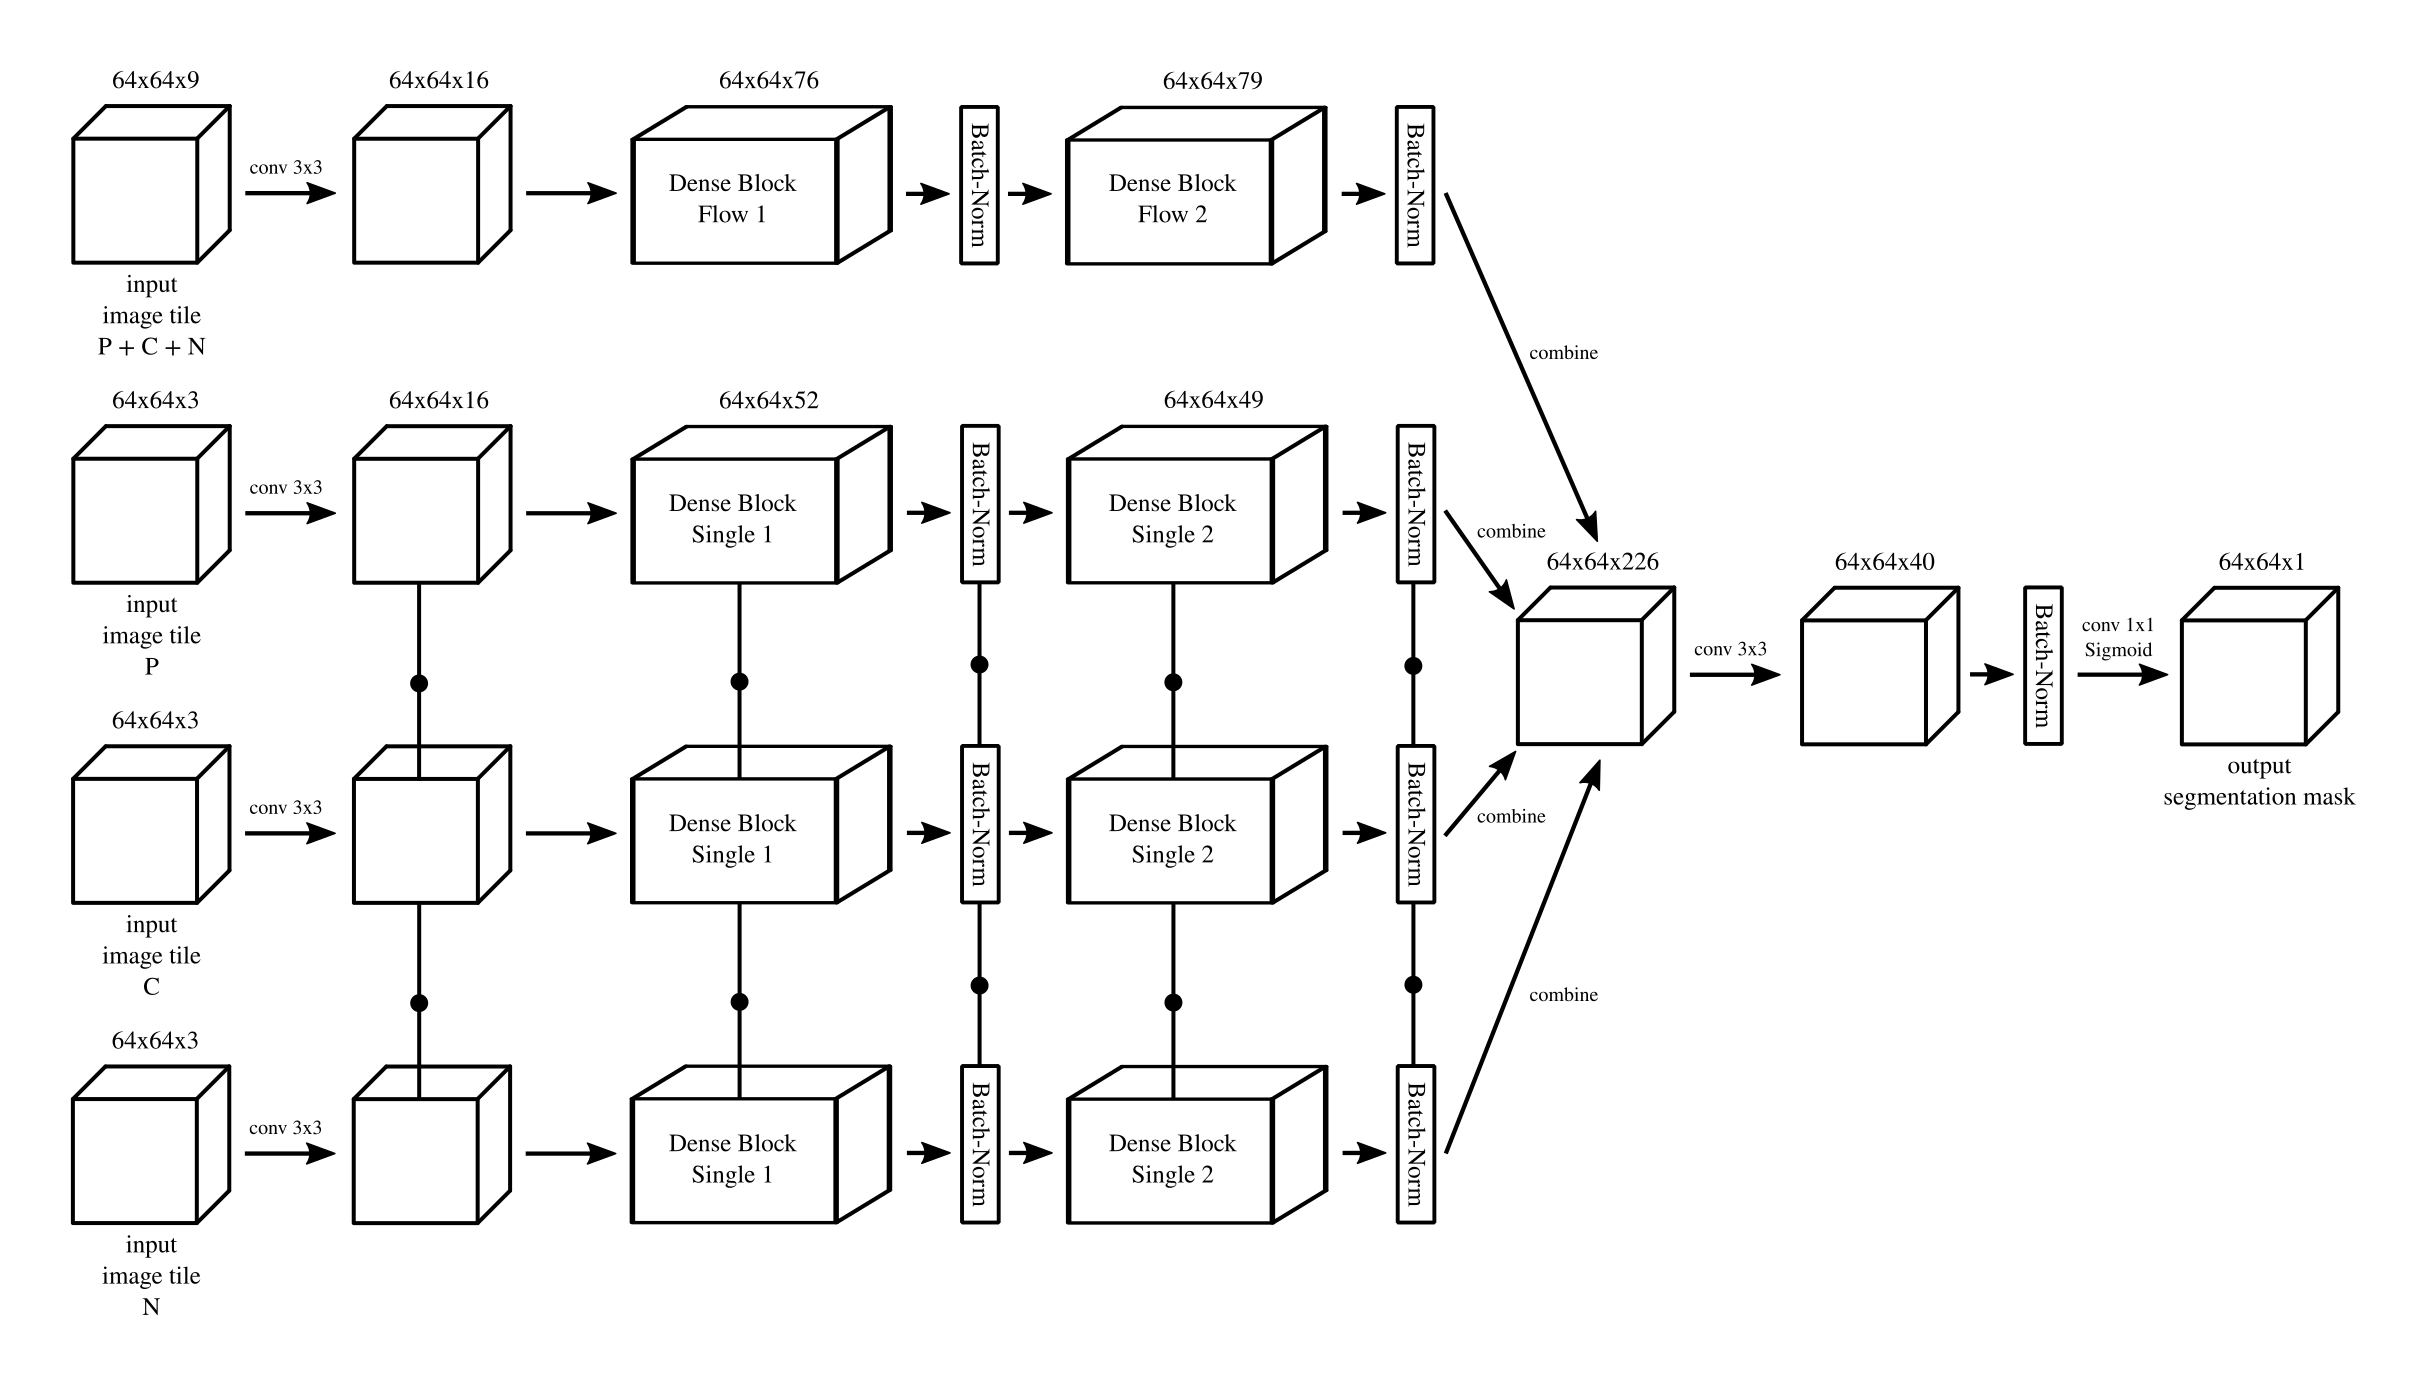
\includegraphics[width=\linewidth]{models_flow/densenet_comb.png}
	\caption[figure]{A "densenet combine"-network. The upper path consists of two densenet blocks and the lower path of two shared denesnet block. The two paths get combined via stacking to achieve a final segmentation mask. We train this architecture on $64\times64$ sized patches.}
	\label{fig:flow_densenet_comb}
	\end{subfigure}
\end{figure}
\begin{figure}[H]
  \ContinuedFloat
  \centering
			\begin{subfigure}{.95\textwidth}
		\centering
		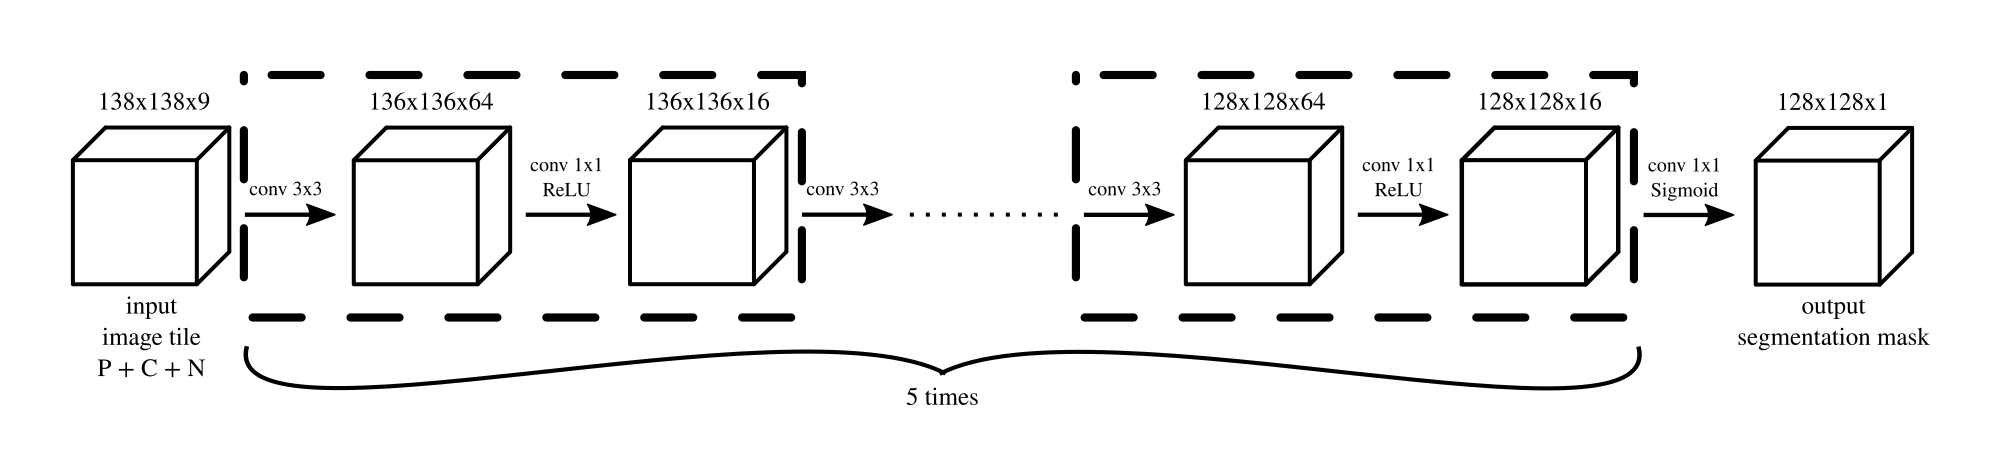
\includegraphics[width=\linewidth]{models_flow/bottleneck.png}
	\caption[figure]{A "bottleneck"-network with five blocks. An additional padding of size 5 was added to each $128\times128$ patch because valid convolution was used.}
	\label{fig:flow_bottleneck}
	\end{subfigure}
		\end{figure}
	\begin{figure}[H]
  \ContinuedFloat
  \centering
				\begin{subfigure}{.95\textwidth}
		\centering
		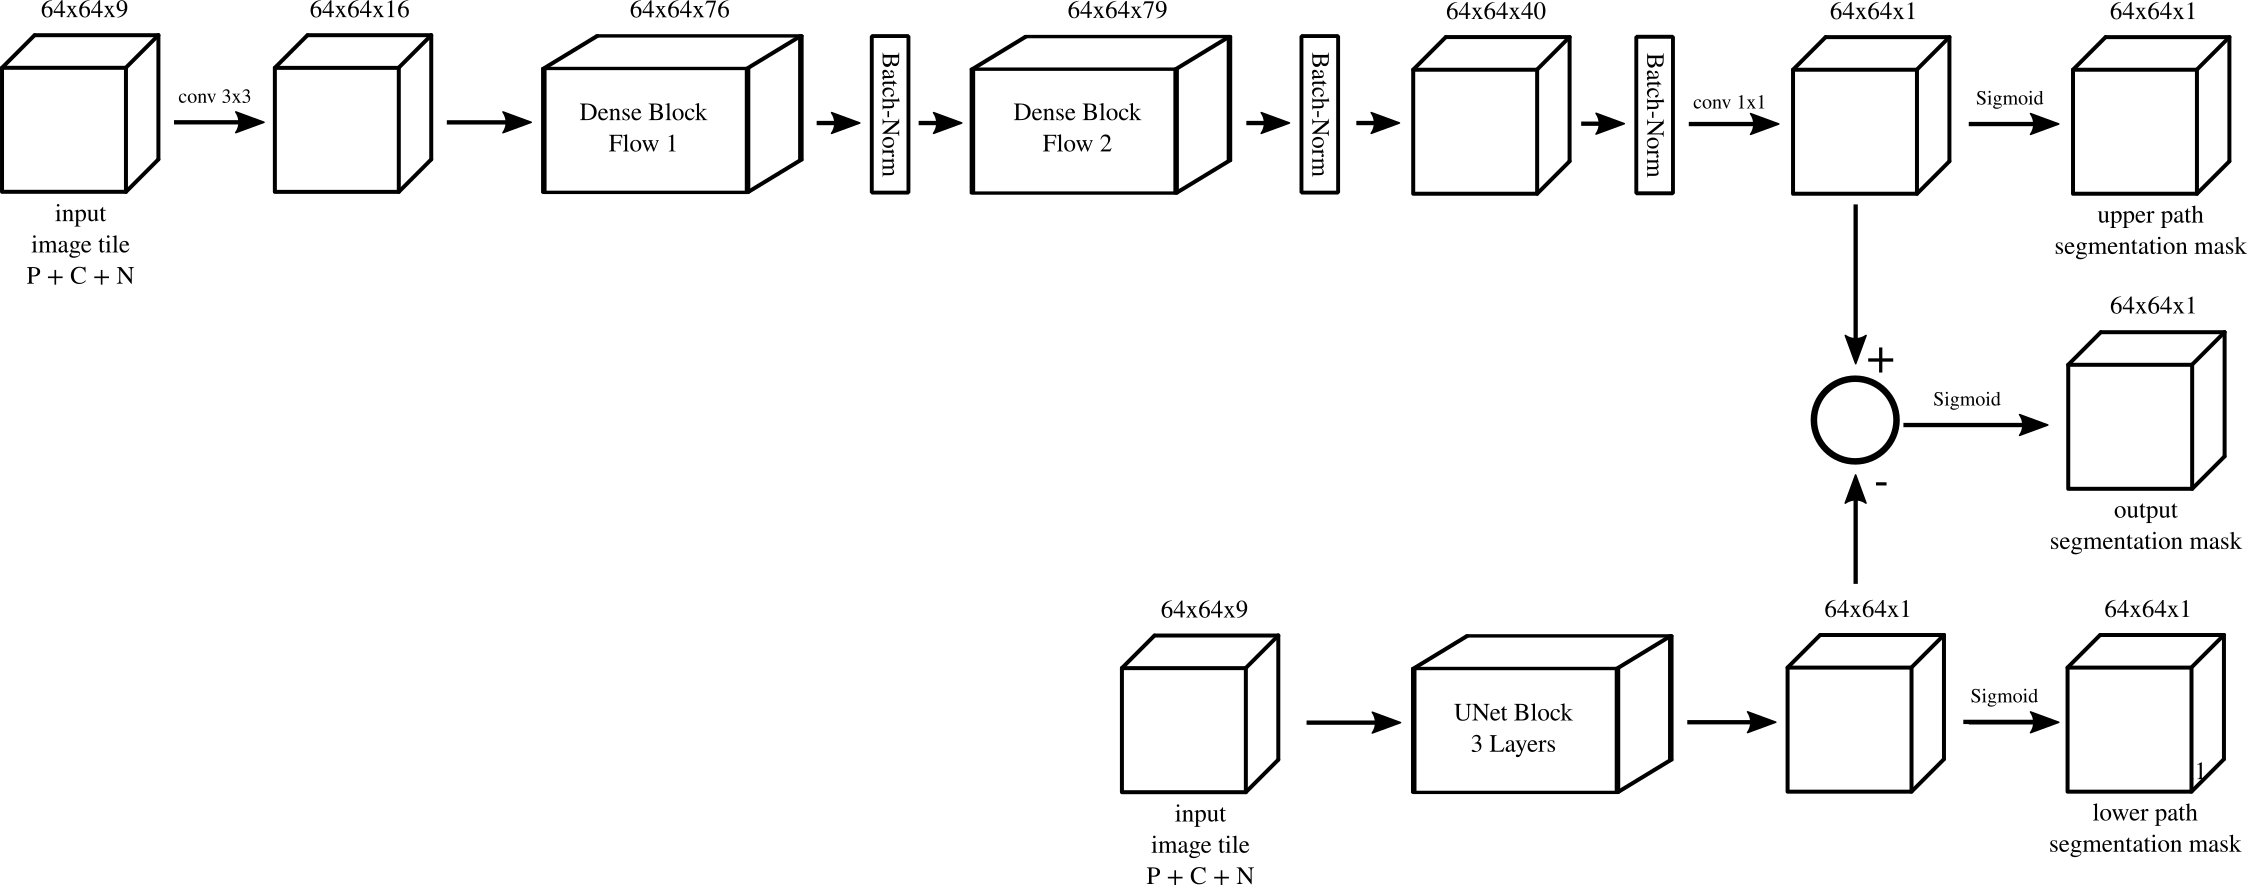
\includegraphics[width=\linewidth]{models_flow/densenet_comb2.png}
	\caption[figure]{A "densenet combine 2"-network. The upper path consists of two densenet blocks and the lower path of an U-Net block with three layers. The intermediate results of the two paths get subtracted to achieve a final segmentation mask. We train this architecture on $64\times64$ sized patches.}
	\label{fig:flow_densenet_comb2}
	\end{subfigure}
	
	\caption[figure]{Different CNN architectures for image segmentation. The "P" and "N" in each Figure~(a)~-~(g), in "image tile P + C + N", stands for previous and next, and means that we use additional information from previous and next image as well. }
	\label{fig:flow_architecutes}
\end{figure}


\subsection{Multiple Warped Input Images}
\label{ssec:num33}

Based on the results of using additional information from previous and next images (Section~\ref{ssec:num532}), we decide to test warped instances of the previous and next image. The results for Section~\ref{ssec:num32} suggest that for sequences with a large optical flow, the tested architectures do not just estimate the impurities but also detect the optical movement. Therefore, we warp the previous and next image to match the current image to suppress the optical flow. For this Section, we use the same architectures as in Section~\ref{ssec:num32}. 

Figure~\ref{fig:warp_1} shows an example of the input images as we use them in Section~\ref{ssec:num32}. In Figure~\ref{fig:warp_2} one can see warped instances of the previous and next image. For this example, the warping can be best seen by comparing the bars of the roof next to the head.

\begin{figure}[H]
	\centering
	\begin{subfigure}{.3\textwidth}
		\centering
		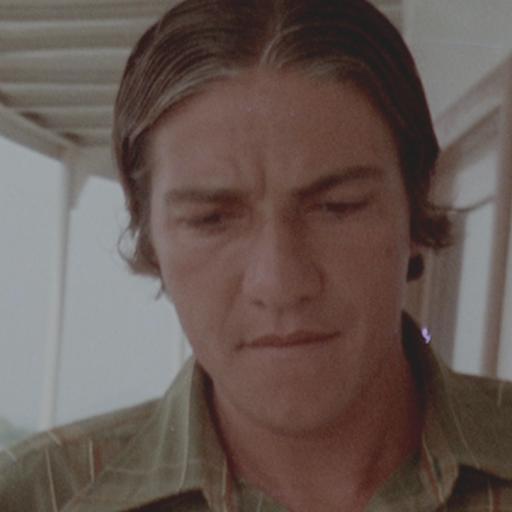
\includegraphics[width=\linewidth]{warp/previous.png}
		\caption[figure]{Previous image}
		\label{fig:warp_prev}
	\end{subfigure}
	\begin{subfigure}{.3\textwidth}
		\centering
		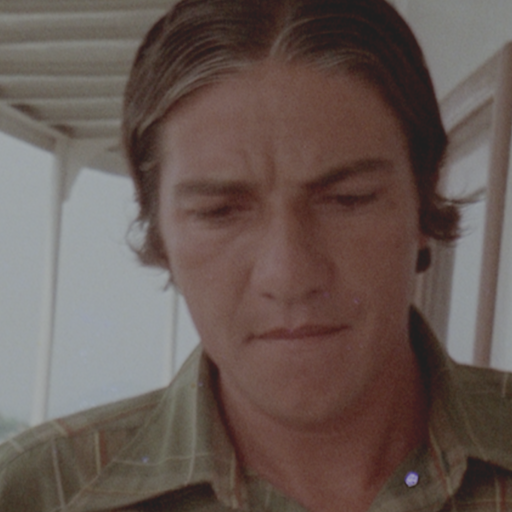
\includegraphics[width=\linewidth]{warp/input.png}
		\caption[figure]{Input image}
		\label{fig:warp_input}
	\end{subfigure}
	\begin{subfigure}{.3\textwidth}
		\centering
		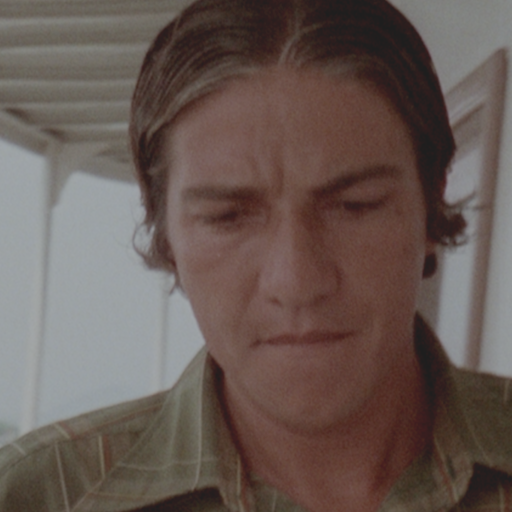
\includegraphics[width=\linewidth]{warp/next.png}
		\caption[figure]{Next image}
		\label{fig:warp_next}
	\end{subfigure}
	\caption[figure]{Example input images as in Section~\ref{ssec:num32}.}
	\label{fig:warp_1}
\end{figure}

\begin{figure}[H]
	\centering
	\begin{subfigure}{.3\textwidth}
		\centering
		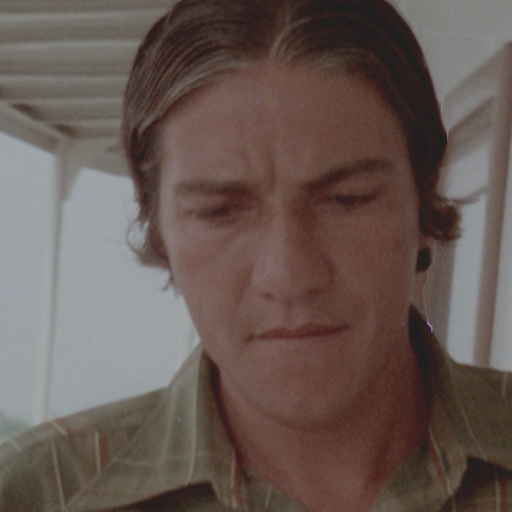
\includegraphics[width=\linewidth]{warp/warpedPrevious.png}
		\caption[figure]{Warped previous image}
		\label{fig:warp_warpprev}
	\end{subfigure}
	\begin{subfigure}{.3\textwidth}
		\centering
		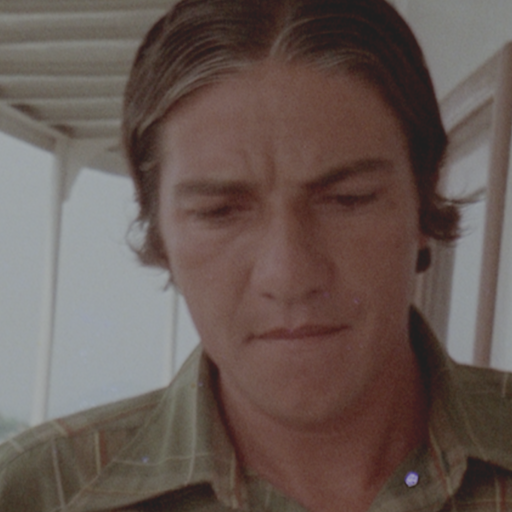
\includegraphics[width=\linewidth]{warp/input.png}
		\caption[figure]{Input image}
		\label{fig:warp_warpinput}
	\end{subfigure}
	\begin{subfigure}{.3\textwidth}
		\centering
		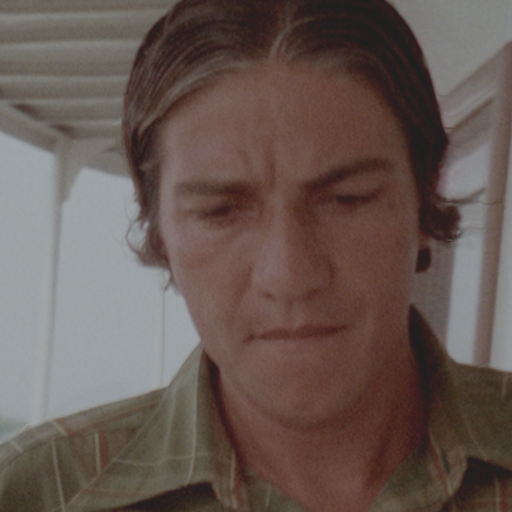
\includegraphics[width=\linewidth]{warp/warpedNext.png}
		\caption[figure]{Warped next image}
		\label{fig:warp_warpnext}
	\end{subfigure}
	\caption[figure]{Example input images for this Section. (a) is a warped instance of Figure~\ref{fig:warp_prev} and (c) a warped instance of Figure~\ref{fig:warp_next}.}
	\label{fig:warp_2}
\end{figure}

We train all the CNN architectures once for the warped image instances and once without warping to see if there is a difference. The results are listed in Section~\ref{ssec:num533}.

\subsection{Regularization Techniques}
\label{ssec:num34}

Techniques to prevent deep learning algorithms from overfitting are called regularizer. The following Sections~\ref{sssec:num341}~-~\ref{sssec:num345} give a description of the different methods used in our CNN models (Section~\ref{ssec:num31}~-~\ref{ssec:num33} and \ref{ssec:num41}).

\subsubsection{Early Stopping}
\label{sssec:num341}
By investigating the trend of test and training error over iterations of deep learning algorithms (Figure~\ref{fig:reg_early_stopping}), one can observe that the training error decreases over iterates, but, the test error first decreases and then increases.
\begin{figure}[H]
	\centering
	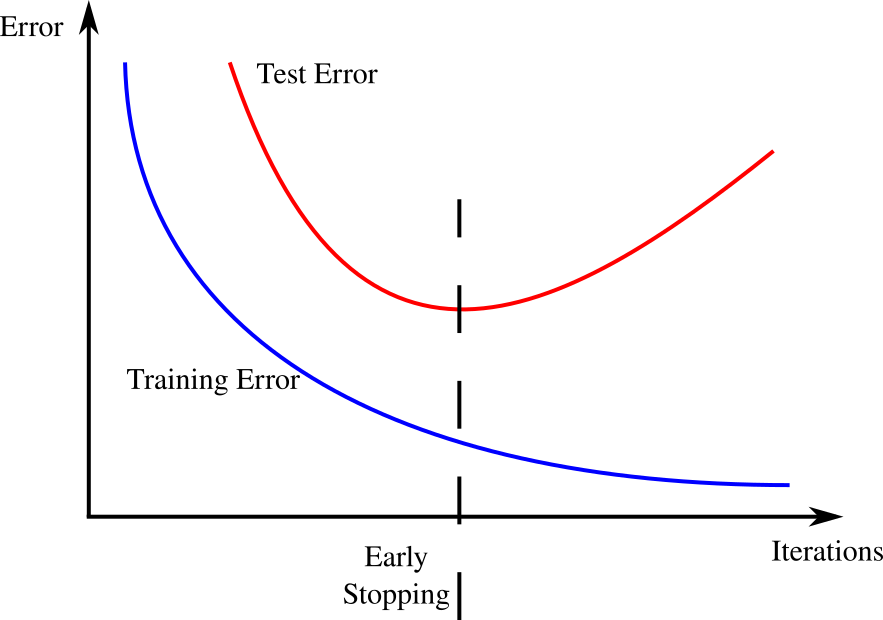
\includegraphics[width=.4\linewidth]{regularization/early_stopping.png}
	\caption[figure]{Trend of training and test error over iterates of deep learning algorithms. The training error is increasing. The test error decreases first and then increases.}
	\label{fig:reg_early_stopping}
\end{figure}
Early stopping now works as follows: we monitor the error on the test set and store the model parameters every time we get a smaller error, after we determined with the number of iterations, we restore our model parameters with the lowest error on the test set. Early stopping acts as a regularizer because with increasing iterations the parameters grow and the effective model capacity grows. 

\subsubsection{Dropout}
\label{sssec:num342}
As Hinton et al.~\cite{Hinton12} state, the idea behind dropout is that neurons can not fully rely on the output of other neurons. So, co-specialization is not possible.

With dropout, a neuron/unit is dropped during training with a probability $1-p$, where $p$ is the so called "keep probability". To drop a unit means, that both in the forward and backward-pass, the unit is ignored (output is set to $0$). For our models we choose a keep probability $p$ of $0.85$.


\subsubsection{$L_2$-Regularization (Weight Decay)}
\label{sssec:num343}

$L_2$-Regularization is a form of adding a parameter norm penalty $\Omega(\textbf{W})$ to the error $E$,~Eq.~\eqref{eq:L2_error}, with $\textbf{W}$ being the weights of our model (the biases are not regularized):
\begin{equation}
\tilde{E}(\textbf{W},D) = E(\textbf{W},D)+\alpha\Omega(\textbf{W})\,,
\label{eq:L2_error}
\end{equation}
with
\begin{equation}
\Omega(\textbf{W})= \frac{1}{2}||\textbf{w}||^2_2
\label{eq:L2_reg}
\end{equation}
and $\textbf{w}$ as the vectorized weights. This added $L_2$-Regularization ,~Eq.\eqref{eq:L2_reg}, leads to a weight decay. For the parameter $\alpha$, we choose a value of $10^{-3}$ for our models.

\subsubsection{Input Normalization}
\label{sssec:num344}

Input normalization is a technique that can speed up learning. We normalize each input feature to have zero-mean and unit-variance, like in Eq.~\eqref{eq:IN}:
\begin{equation}
\tilde{x}^{(n)}_i= \frac{x^{(n)}_i-\bar{x}_i}{\sigma_{x_i}}\,,
\label{eq:IN}
\end{equation}
with $\bar{x}_i$ as the mean value of the $i^{th}$-feature of $x$, $x_i$, 
\begin{equation}
\bar{x}_i = \frac{1}{N}\sum_{j=1}^{N}x^{(j)}_i\,,
\label{eq:mean}
\end{equation}
and $\sigma_{x_i}$ as the standard deviation of the $i^{th}$-feature of $x$, $x_i$,  
\begin{equation}
\sigma_{x_i} = \sqrt{\frac{1}{N}\sum_{j=1}^{N}(x^{(j)}_i-\bar{x}_i)^2}\,.
\label{eq:std}
\end{equation}

\subsubsection{Batch Normalization}
\label{sssec:num345}
The output of a layer can be interpreted as the input of the next layer. 
In batch normalization, this normalization (like in Section~\ref{sssec:num344}) is done to the output of each layer for the current batch. 
As Ioffe et al.~\cite{Ioffe15} mention, this technique leads to better learning dynamics. Batch normalization can be seen as an intermediate layer that linearly transforms the output of a layer.  



\section{Image In-painting}
\label{sec:num4}

In this Section follows a description of our methods and approaches for the removing of impurities by image in-painting. We try out different approaches. In Section~\ref{ssec:num41} we perform image in-painting based on the generated segmentation masks of the Densenet Combined model, since this model achieves best results (see Section~\ref{ssec:num532}). In Section~\ref{ssec:num42} follows an approach where we do not use any segmentation mask at all. 

\subsection{With Segmentation Mask}
\label{ssec:num41}

As already mentioned, in this Section we perform image in-painting by using our previously generated segmentation mask. Again, we focus on machine learning approaches namely CNNs but compare these against a diffusion based image in-painting. Section~\ref{sssec:num411} gives an overview of CNN architectures that are trained for a single color channel. Section~\ref{sssec:num412} gives an theoretical overview on diffusion based image in-painting, as well as the exact used approach. 
The results of the different image in-painting approaches can be seen in Section~\ref{sssec:num541}.

\subsubsection{CNN}
\label{sssec:num411}

Based on the results of Section~\ref{ssec:num532} we decide to test various densenet approaches. Additionally, as seen in Section~\ref{ssec:num532}, we use information from previous and next images as well. We train all following networks on quintuples of: previous~-~current~-~next~images~-~ground-truth-masks + ground-truth~in-painting.


It should be mentioned that we use ReLU activation functions between layers and a ReLU output activation function to perform image in-painting. We also apply regularization techniques, namely early stopping (Section~\ref{sssec:num341}), dropout (Section~\ref{sssec:num342}) and $L_2$-regularization (Section~\ref{sssec:num343}). We choose the $L_2$-loss for computing the loss/error between predicted and ground-truth in-painting.  For \ref{fig:paint_densenet} we calculated the loss just over masked pixels. And, we copy valid input pixel values into the predicted in-painting.

Since we train on a single color channel, we also have to perform the testing on each color channel separately and combine the intermediate results.


The different networks (Figure~\ref{fig:paint_architectures}) tested are: \begin{enumerate*}[label=(\alph*)] \item a network based on the work of Huang et al.~\cite{Huang16} that consists of five sub-blocks, and \item a network with two paths, where we add the input image in the end. This network is also based on the work of Huang et al.~\cite{Huang16} and for this network we use a linear output activation function.\end{enumerate*}



\begin{figure}[H]
\centering
	\begin{subfigure}{.95\textwidth}
	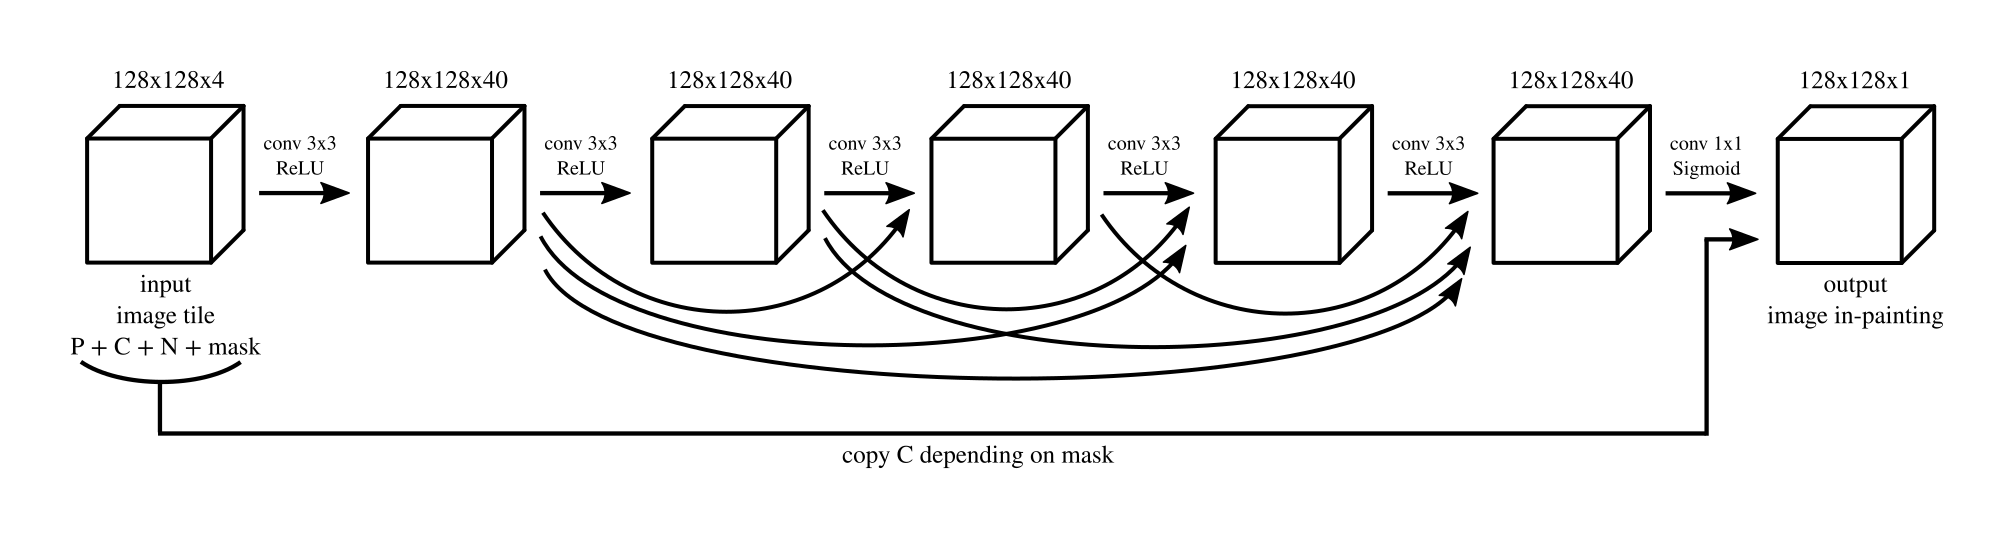
\includegraphics[width=\linewidth]{models_painting/densenet.png}
	\caption[figure]{A "densenet copy"-network for image in-painting with five sub-blocks.}
	\label{fig:paint_densenet}
	\end{subfigure}
\end{figure}
\begin{figure}[H]
  \ContinuedFloat
  \centering
  \begin{subfigure}{.95\textwidth}
	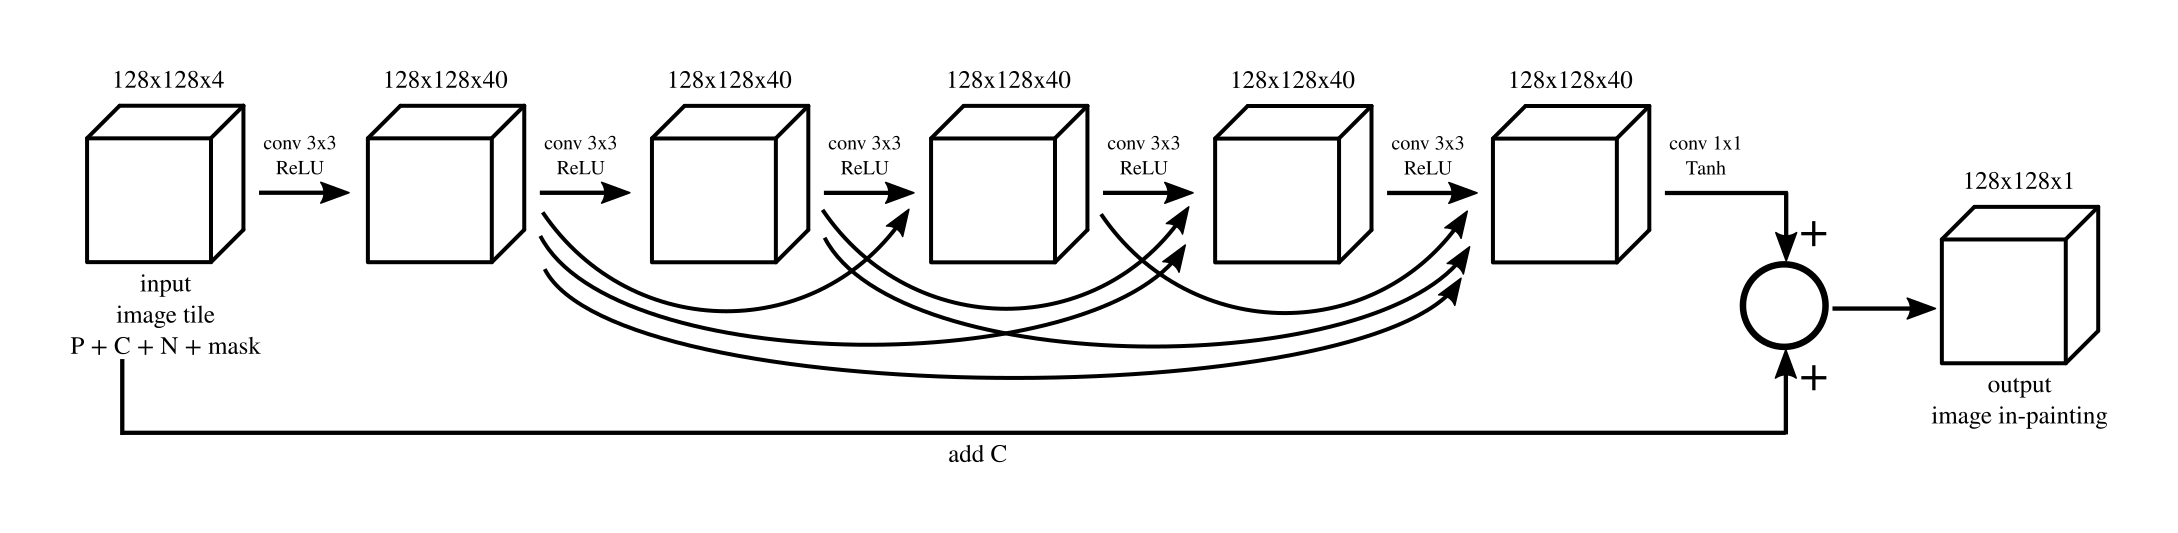
\includegraphics[width=\linewidth]{models_painting/densenet2.png}
	\caption[figure]{A "densenet add"-network for image in-painting with five sub-blocks.}
	\label{fig:paint_densenet2}
	\end{subfigure}
  	
	\caption[figure]{Different CNN architectures for image in-painting with previously generated segmentation mask.}
		\label{fig:paint_architectures}
\end{figure}


\subsubsection{Perona-Malik In-painting}
\label{sssec:num412}
The second image in-painting approach is based on a modified version of coherence-enhancing image diffusion. The theoretical basis are after Perona~and~Malik~\cite{Perona90} or Weickert~\cite{weickert98}. Now follows a description of the used method for one color channel.

Let $u : \Omega \rightarrow \mathbb{R}$ be the image function, with $  \Omega \subset \mathbb{R}^2$ the image domain. The basic diffusion equation is given by: \begin{equation}\frac{\partial u}{\partial t}=\text{div}(\nabla u)\,.
\label{eq:PM_basic}
\end{equation}
Eq.~\eqref{eq:PM_basic} is a PDE and is used to describe \textit{isotropic} diffusion. To increase the modeling accuracy, a so-called diffusion tensor $D$ is introduced into Eq.~\eqref{eq:PM_basic}:
\begin{equation}
\frac{\partial u}{\partial t} = \text{div}(D\nabla u)\,.
\label{eq:PM_basic2}
\end{equation}
Eq.~\eqref{eq:PM_basic2} describes \textit{anisotropic} diffusion and the diffusion tensor $D$ models rate of diffusion in different directions. If $D$ is the identity matrix, we again obtain \textit{isotropic} diffusion. 

Coherence-enhancing diffusion leads the diffusion along coherent regions, similar structured regions, in our case edge directions. We achieve this, by using a structure tensor $S$ ($2 \times 2$ matrix). The structure tensor is able to give for every pixel information about its surrounding structure, and is calculated via:
\begin{equation}
S=G_\sigma *
\begin{bmatrix}
    \tilde{u}^2_x       & \tilde{u}_x \tilde{u}_y   \\
   \tilde{u}_x \tilde{u}_y & \tilde{u}^2_y
\end{bmatrix}\,,
\label{eq:PM_S}
\end{equation}
with subscripts denoting directional derivatives. $G_\sigma$ is a Gaussian smoothing kernel with $\sigma_t$, and $\tilde{u}$ is a Gauss-filtered version of $u$ with $\sigma_g$. The eigenvalues $\mu_1 , \mu_2$ and eigenvectors $\nu_1 , \nu_2$ of the structure tensor $S$ give information about the local structure of the image, with the eigenvalues determining the magnitude of the grayvalue variation, the corresponding eigenvector giving the direction of the grayvalue variation:
\begin{enumerate}
\item $\mu_1 , \mu_2$ both small: flat region,

\item $\mu_1 \gg \mu_2$ or vice-versa: strong grayvalue variation in one direction, \textit{i.e.} image edge,
\label{enum:PM_b}

\item $\mu_1 , \mu_2$ both large: strong grayvalue variation in two directions,\textit{i.e.} image corner,
\end{enumerate}
with this information we will guide the diffusion process.

The diffusion tensor $D$ is calculated as:
\begin{equation}
D=\begin{bmatrix}
    \nu_1 & \nu_2
   \end{bmatrix}   
\begin{bmatrix}
    \lambda_1       & 0  \\
   0 & \lambda_2
\end{bmatrix}
\begin{bmatrix}
    \nu_1^T \\ \nu_2^T
   \end{bmatrix}\,,
\label{eq:PM_D}
\end{equation}
using a small constant $\alpha > 0$, $\lambda_1$ and $\lambda_2$ are given as
\begin{equation}
\begin{cases}
     \lambda_1=\alpha\\
     \lambda_2=\alpha + (1-\alpha)(1-g(|\mu_1-\mu_2|))   \end{cases}
\end{equation}
and $g(s)=e^{-\frac{s^2}{2\gamma^2}}$ with a parameter $\gamma$.

We solve Eq.~\eqref{eq:PM_basic2} with a semi-implicit approach. Since we are in the discrete world, an image of size $M \times N$ is represented as a vector $U \in \mathbb{R}^{MN}$, the time derivative $\frac{\partial u}{\partial t}$ and $K \in \mathbb{R}^{2MN\times MN}$ the equivalent to $\nabla$ approximated by finite differences, $D(U^t) \in \mathbb{R}^{2MN\times2MN}$ the diffusion tensor, $\tau$ the time discretisation step and since $\text{div} = -\nabla^T$ we then can write Eq.~\eqref{eq:PM_basic2} as
\begin{equation}
\frac{U^{t+1}-U^t}{\tau}=-K^TD(U^t)KU^{t+1}\,.
\label{eq:PM_basic3}
\end{equation}
Re-writting Eq.~\eqref{eq:PM_basic3} and the introduction of a diagonal mask matrix $Q \in \mathbb{R}^{MN \times MN}$ that highlights pixels for in-painting, and $ \hat{Q}$ the inverse of $Q$ for highlighting preserved regions and solving for $U^{t+1}$ leads to the image in-painting equation for one channel:

\begin{equation} \label{eq:PM_final}
\begin{split}
Q(U^{t+1}-U^t)+\hat{Q}\tau K^TD(U^t)K U^{t+1} &= 0 \\
Q U^{t+1}-Q U^t+\hat{Q}\tau K^TD(U^t)K U^{t+1} &= 0 \\
 (Q+\hat{Q} \tau K^TD(U^t)K) U^{t+1} &= Q U^t\\
  U^{t+1} &= (Q+\hat{Q}\tau K^TD(U^t)K)^{-1}QU^t\,.
\end{split}
\end{equation}


The extension of this single channel image in-painting to color images is done by applying the diffusion for each channel. To avoid artifacts many different approaches exist. As {\AA}str{\"o}m et al.~\cite{aastrom11} state one could use a different color space, like HSV instead of RGB, use one diffusion tensor for each channel that is computed as the weighted average sum of the structure tensors for each color channel, use a different structure tensor for each channel, \textit{etc.} We choose the approach of using the weighted sum over all channels for the structure tensor and use this for each channel.

\subsection{Without Segmentation Mask}
\label{ssec:num42}

As an additional variant for image in-painting, we decide to test the estimation of the corrupted pixels without the help of the segmentation mask. This is due to the fact that the provided ground truth segmentation masks are of poor quality. Again, we test different densenet approaches and we use use information from previous and next images as well. But now we train all following networks on triples of: previous~-~current~-~next~images~ + ground-truth~in-painting, so without a mask.


It should be mentioned that we use ReLU activation functions between layers and a linear output activation function to perform image in-painting. We do not apply any regularization techniques. We choose the $L_2$-loss for computing the loss/error between predicted and ground-truth in-painting.  For the first two networks we train on color images (Figures~\ref{fig:inpai6}~and~\ref{fig:inpai7}). The model in Figure~\ref{fig:inpai5} gets trained on a single color channel, so we also have to perform the testing on each color channel separately and combine the intermediate results.


The different networks (Figure~\ref{fig:paint_architectures2}), all based on the work of Huang et al.~\cite{Huang16}, tested are: \begin{enumerate*}[label=(\alph*)] \item a network that consists of five sub-blocks and that uses color images as an input, \item a network that consists of two shared densenet blocks for each color channel. This network also uses color images as an input. And, \item a network similar to (a) but this time we train and test on single color channels.\end{enumerate*} For all networks we add the input image in the end to achieve a final in-painted image. The results of these different image in-painting approaches can be seen in Section~\ref{sssec:num542}.


\begin{figure}[H]
\centering
	\begin{subfigure}{.95\textwidth}
	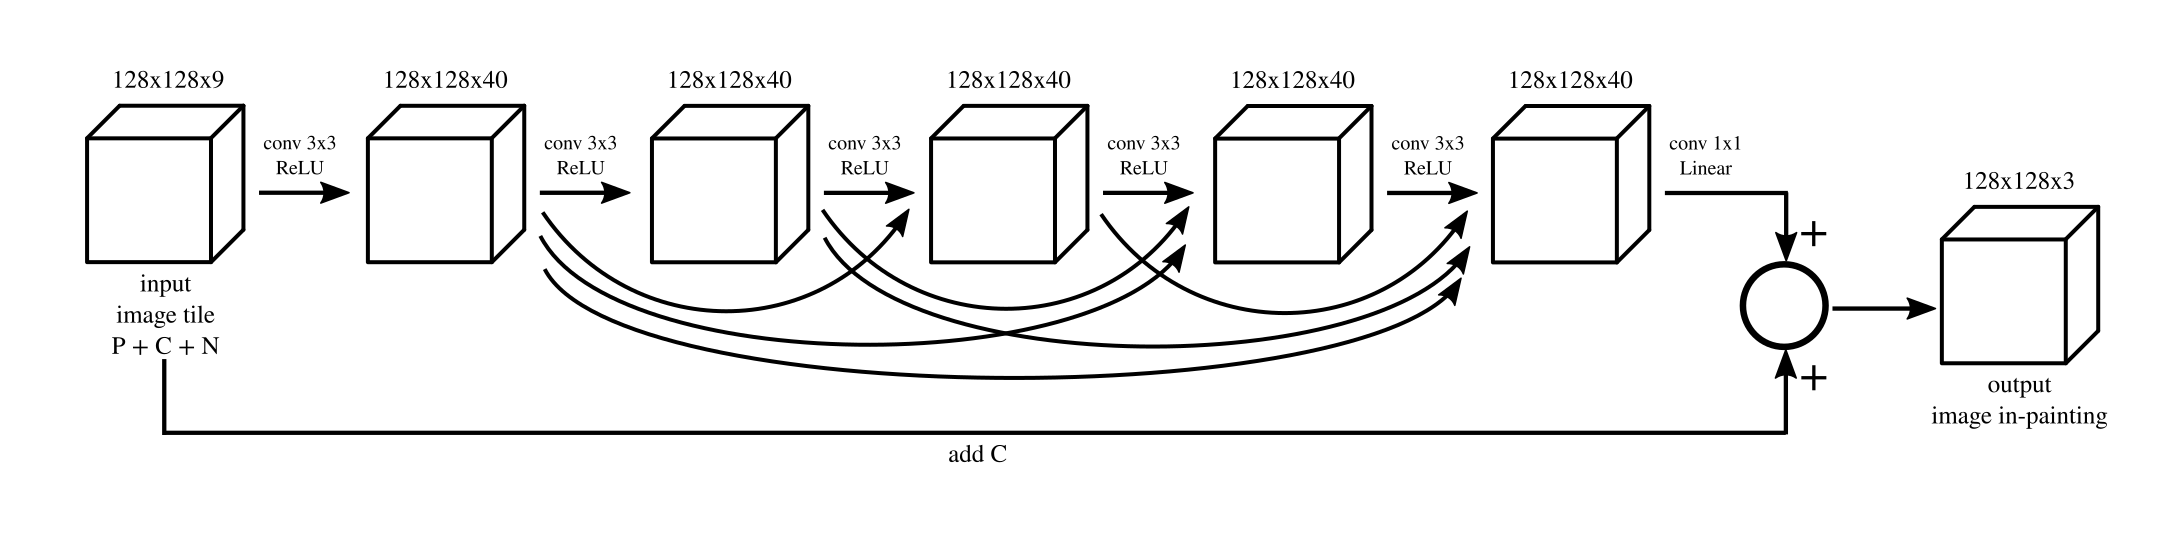
\includegraphics[width=\linewidth]{models_painting_warp/inpai6.png}
	\caption[figure]{A "densenet add"-network for image in-painting with five sub-blocks (Training and testing with color images).}
	\label{fig:inpai6}
	\end{subfigure}
\end{figure}
\begin{figure}[H]
  \ContinuedFloat
  \centering
  \begin{subfigure}{.95\textwidth}
	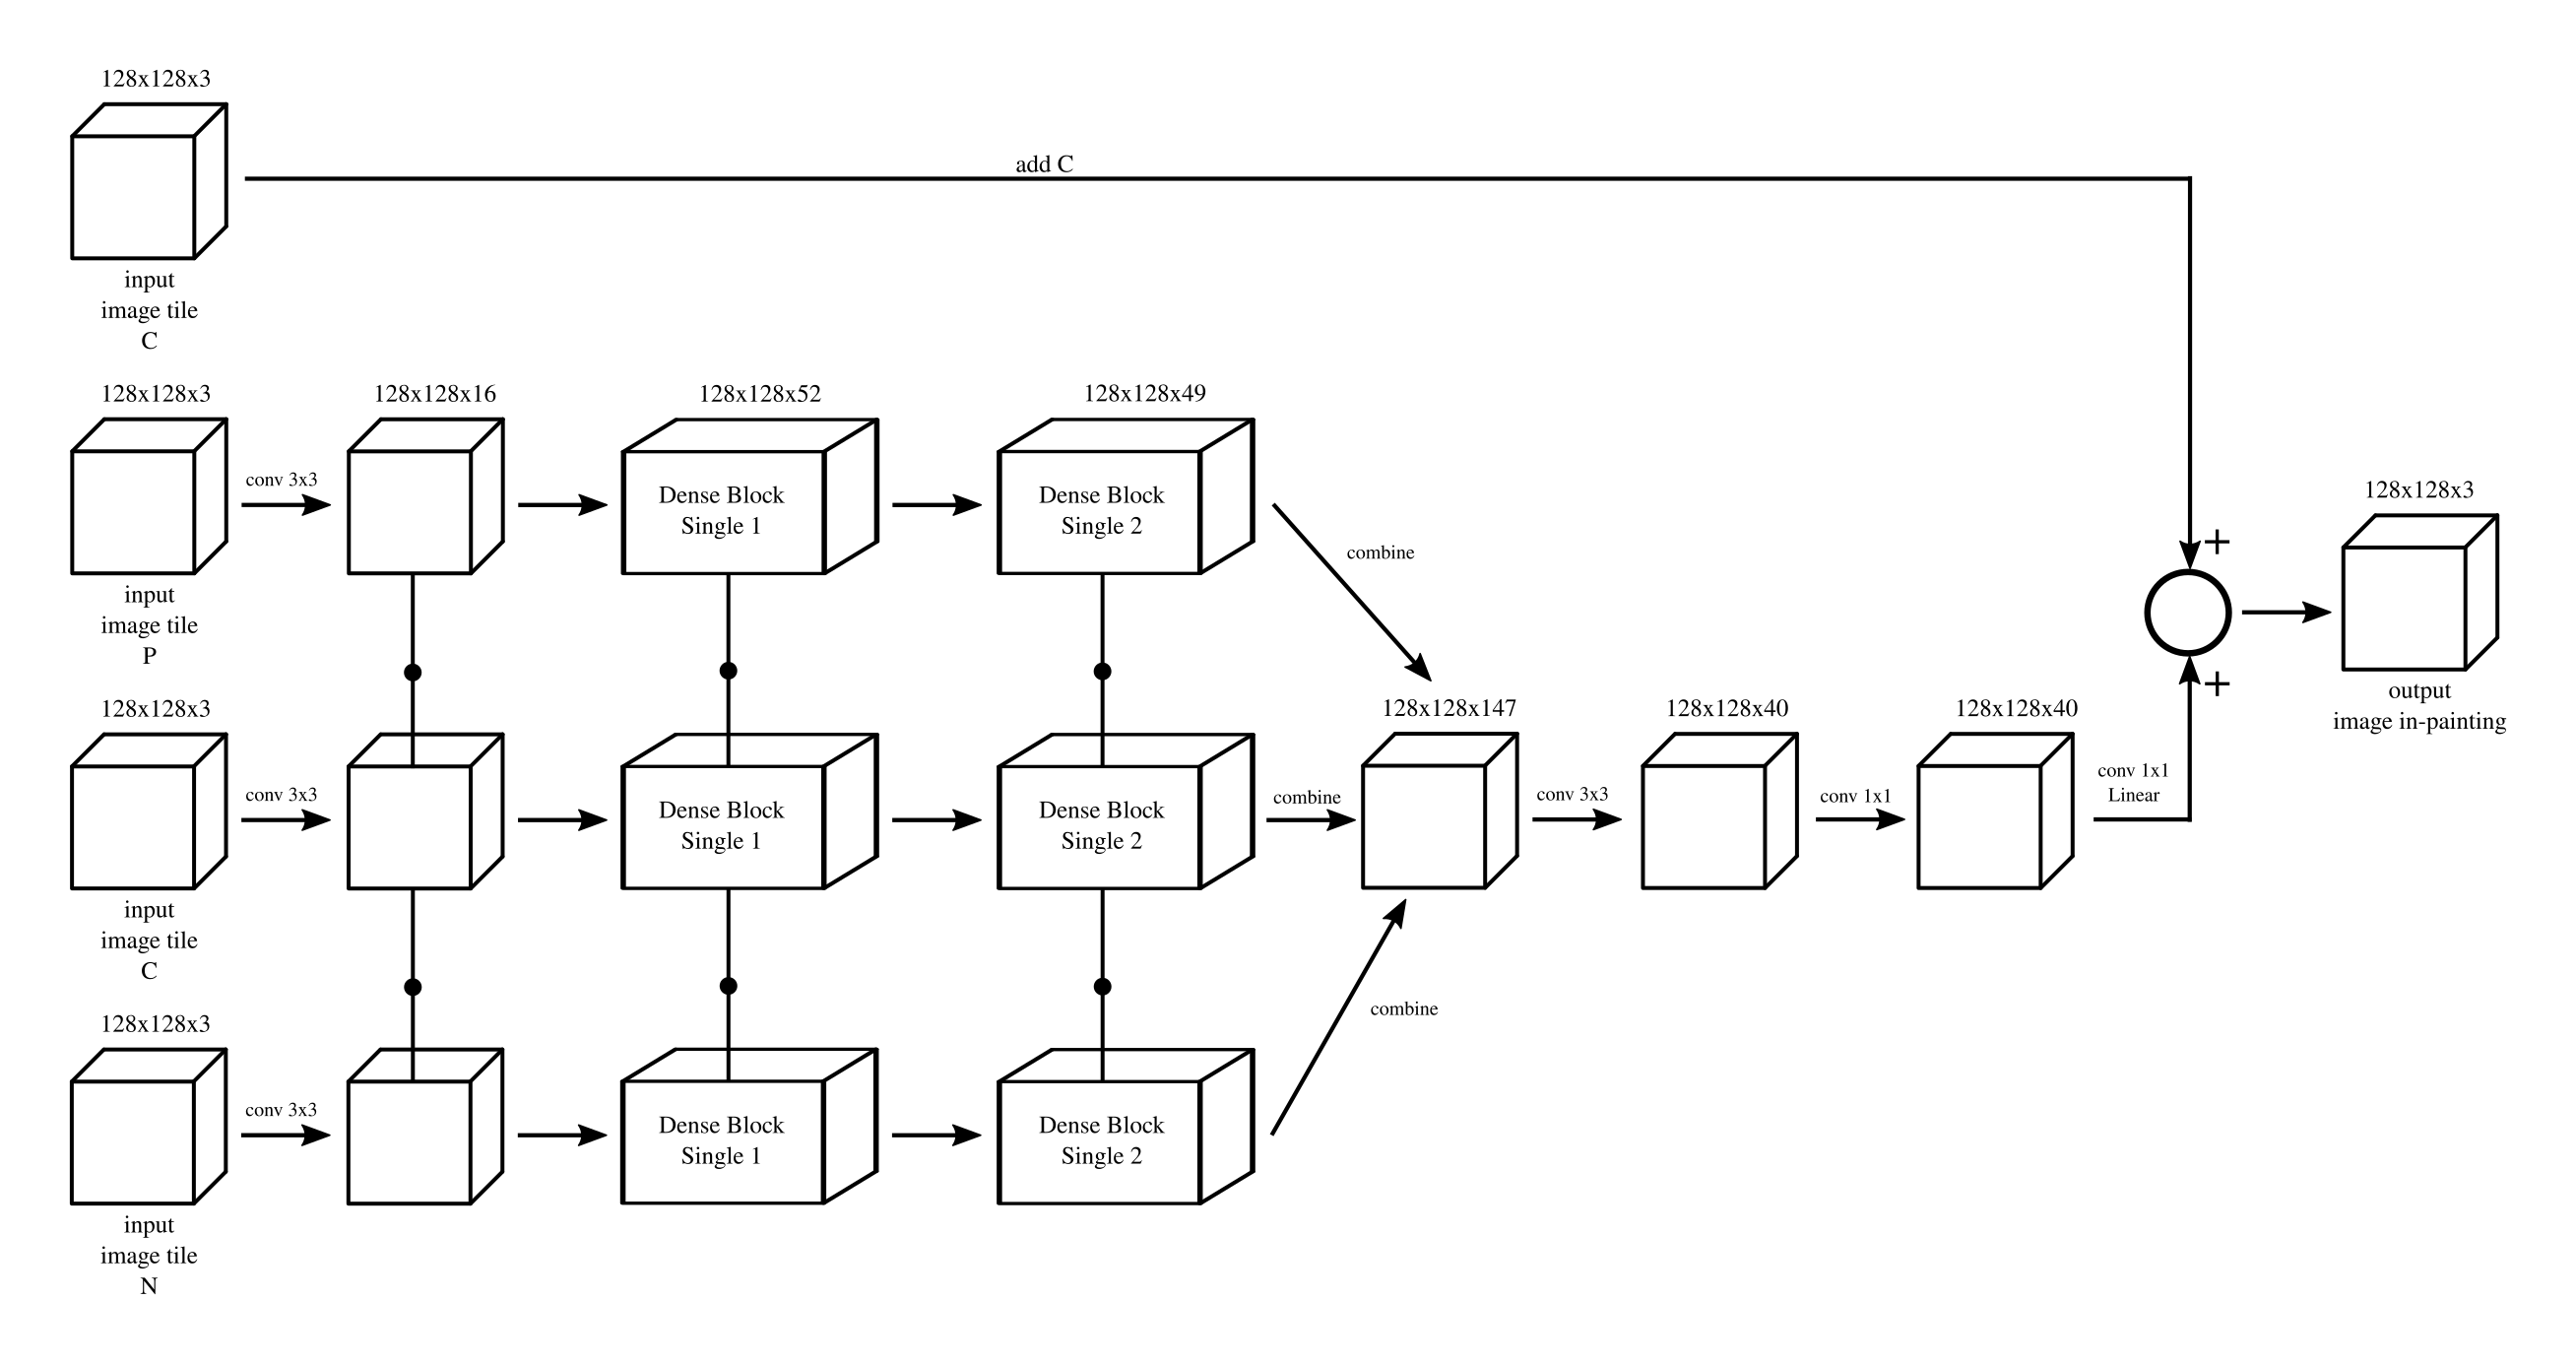
\includegraphics[width=\linewidth]{models_painting_warp/inpai7.png}
	\caption[figure]{A "densenet combine add"-network for image in-painting with two shared densenet blocks for each color channel (Training and testing with color images).}
	\label{fig:inpai7}
	\end{subfigure}

\end{figure}
\begin{figure}[H]
  \ContinuedFloat
\centering
	\begin{subfigure}{.95\textwidth}
	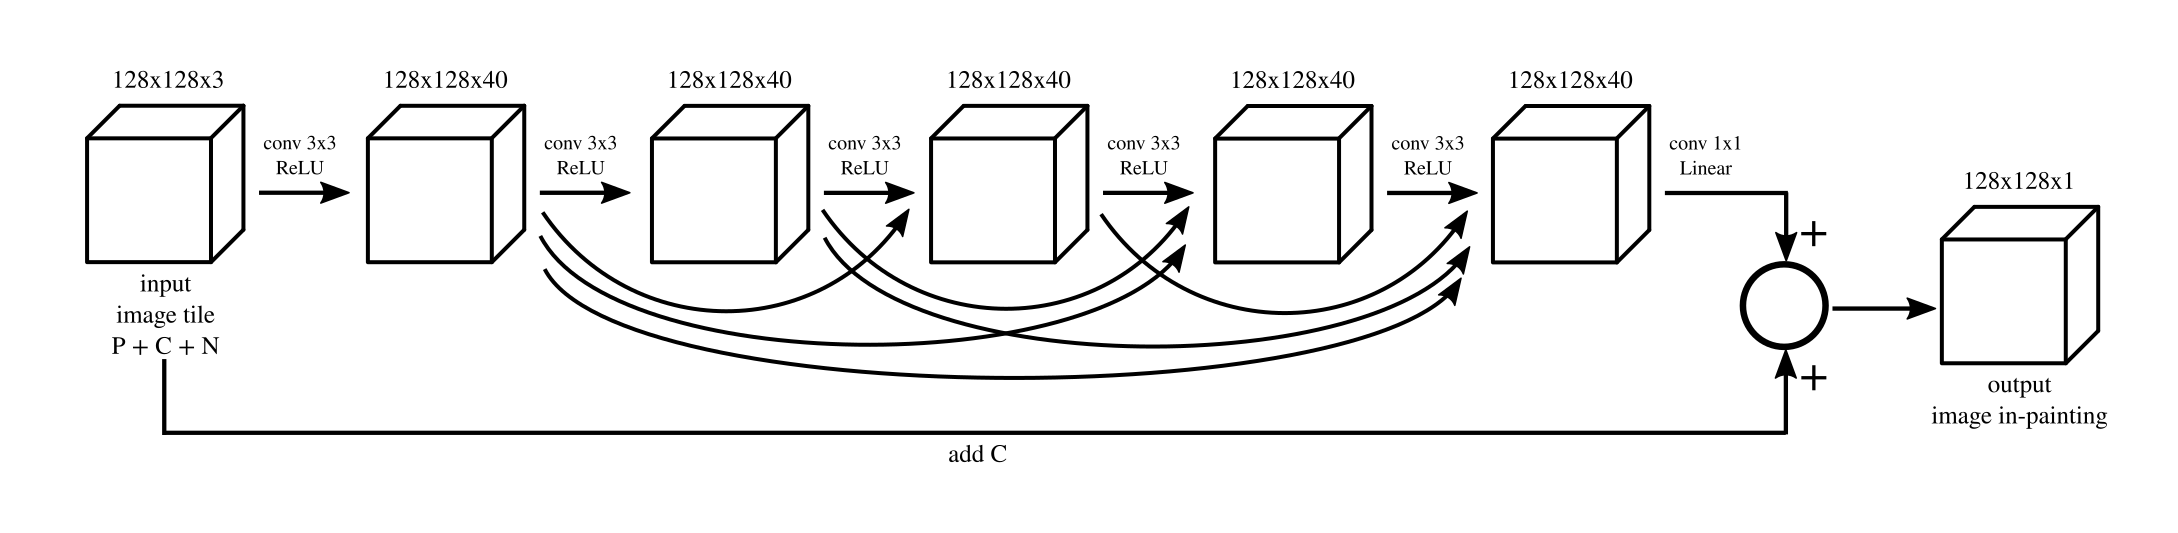
\includegraphics[width=\linewidth]{models_painting_warp/inpai5.png}
	\caption[figure]{A "densenet add"-network for image in-painting with five sub-blocks (Training and testing with  single color channels).}
	\label{fig:inpai5}
	\end{subfigure}
	
	  	
	\caption[figure]{Different CNN architectures for mask-less image in-painting.}
		\label{fig:paint_architectures2}
\end{figure}


\section{Evaluation}
\label{sec:num5}

We evaluate our different approaches with ground-truth images from HS-Art~\cite{hs-art}. A description of this dataset follows in Section~\ref{ssec:num51}. The needed implementation details for the evaluation are stated in Section~\ref{ssec:num52} and in Section~\ref{ssec:num53} our results are presented.

\subsection{Dataset}
\label{ssec:num51}
HS-Art~\cite{hs-art} provides us with a total of 173 image sequences. Per sequence we get an input image (current image) that is corrupted, the previous image in the sequence, the next image in the sequence, the ground-truth segmentation mask, highlighting impurities in the current image as well as ground truth image in-painting results of the current image. Each image is of size $512 \times 512$. For 77 out of these 173 image sequences we additionally have warped instances of the previous and next image, these sequences are used to evaluate Section~\ref{ssec:num33} and \ref{ssec:num42}. For Section~\ref{ssec:num31},~\ref{ssec:num32}~and~\ref{ssec:num41} we use the other 96 image sequences.

For training and evaluation of our CNN approaches we split the sequences into $80\%$ training sequences and $20\%$ test sequences. The training is done on patches of size $128 \times 128$, unless otherwise stated, and we train on patches were atleast $1\%$ and at most $80\%$ pixels are impure.

For the image segmentation task of using multiple input images (Section~\ref{ssec:num32}) we further categorize our test set into sets that have: \begin{enumerate*}[label=(\roman*)] \item ground-truth masks with large areas, \item ground-truth masks with small areas, \item sequences with large flow, and \item sequences with small flow.\end{enumerate*}

We also perform dataset augmentation to get more data for training. Here we perform mirroring of the images and masks as well as a flow reversal by exchanging previous and next image.


\subsection{Implementation Details}
\label{ssec:num52}

The different parameters used for our CNN approaches are listed either in Section~\ref{ssec:num34} or in the corresponding model definitions. Additionally, we use the ADAM-optimizer with a learning rate of $10^{-3}$ to train other models.

For the Perona-Malik image in-painting approach (Section~\ref{ssec:num42}) we use the following values for the parameters:
$\alpha$ = 0.005, $\gamma$ = 0.001, $\tau$ = 5, end time = 15, $\sigma_g$ = 0.7 and $\sigma_t$ = $1.5$.

The project was realized in python and we used the Tensorflow API to implement our CNN approaches. The training and testing was done on a NVidia Geforce Titan X.
			

\subsection{Results for Image Segmentation}
\label{ssec:num53}

In the following Sections we list the results of image segmentation using a single image (Section~\ref{ssec:num531}), additional information from previous and next images (Section~\ref{ssec:num532}) and additional information by using warped instances of previous and next images (Section~\ref{ssec:num533}).
\subsubsection{Single Input Image}
\label{ssec:num531}
The results in Figure~\ref{fig:resu_single} suggest that the information given in just a single current image is not enough for a sufficient learning and estimating of the segmentation mask.
Therefore, we add additional information by using the previous and next image frames for all additional approaches.

\begin{table}[ht!]\begin{center}
 \setlength{\tabcolsep}{1pt}
 \begin{tabular}{ c c c c c}

%\begin{tabular}{p{3cm}p{3cm}p{3cm}p{3cm}p{3cm}}
 %\multicolumn{}{|c|}{Country List} \\

 
 
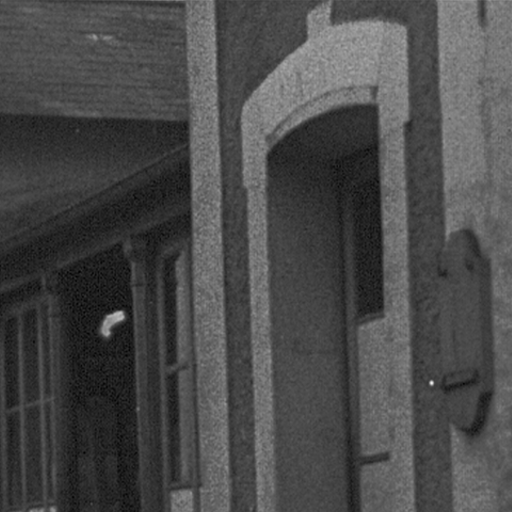
\includegraphics[width=.17\linewidth]{results_single/1000iter_early_combine/cnn_tests/cnn_tests0/input.png} & 
		\setlength{\fboxrule}{0.5pt}
        \setlength{\fboxsep}{0pt}
        \framebox{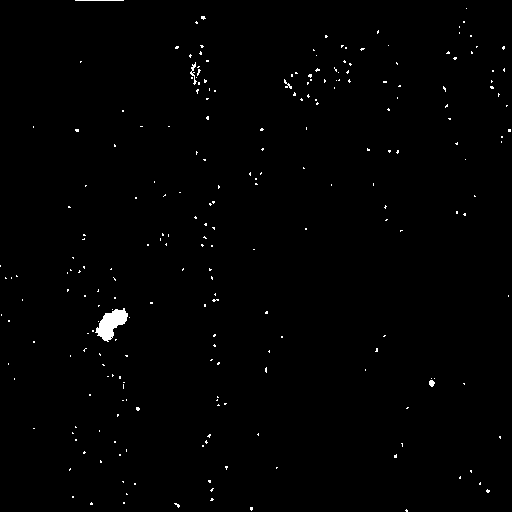
\includegraphics[width=.17\linewidth, decodearray={1 0 1 0 1 0}]{results_single/1000iter_early_combine/cnn_tests/cnn_tests0/GT_mask.png}} &
        \setlength{\fboxrule}{0.5pt}
        \setlength{\fboxsep}{0pt}
        \framebox{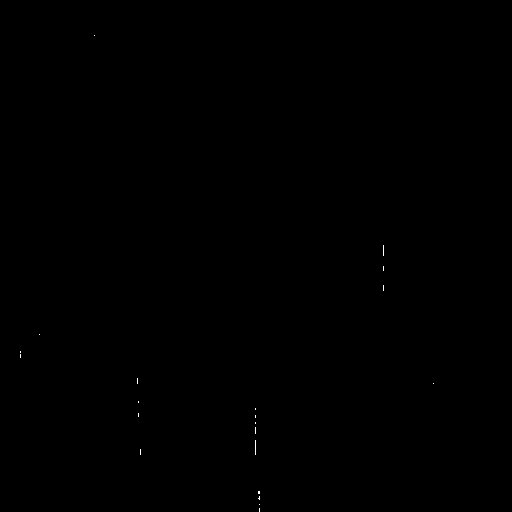
\includegraphics[width=.17\linewidth, decodearray={1 0 1 0 1 0}]{results_single/1000iter_early_combine/cnn_tests/cnn_tests0/pred_mask_TH.png}} & 	
        \setlength{\fboxrule}{0.5pt}
        \setlength{\fboxsep}{0pt}		
        \framebox{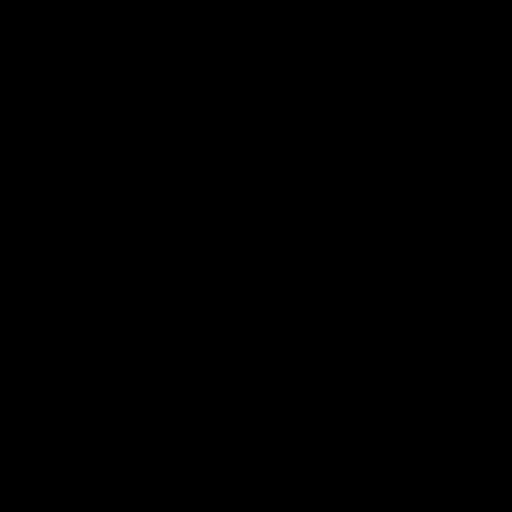
\includegraphics[width=.17\linewidth, decodearray={1 0 1 0 1 0}]{results_single/1000iter_unet/cnn_tests/cnn_tests0/pred_mask_TH.png}} & 
        \setlength{\fboxrule}{0.5pt}
        \setlength{\fboxsep}{0pt}
        \framebox{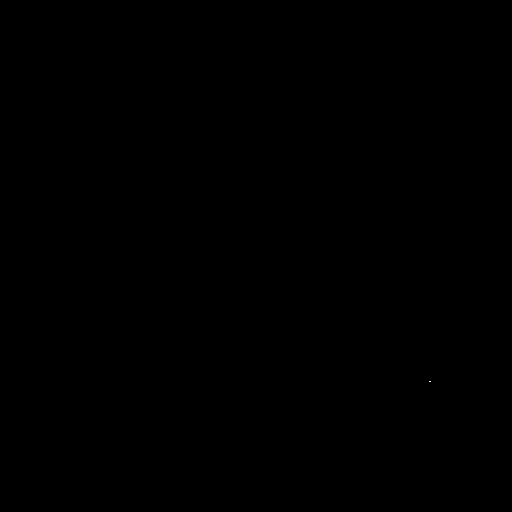
\includegraphics[width=.17\linewidth, decodearray={1 0 1 0 1 0}]{results_single/1000iter_densenet/cnn_tests/cnn_tests0/pred_mask_TH.png}}\\
  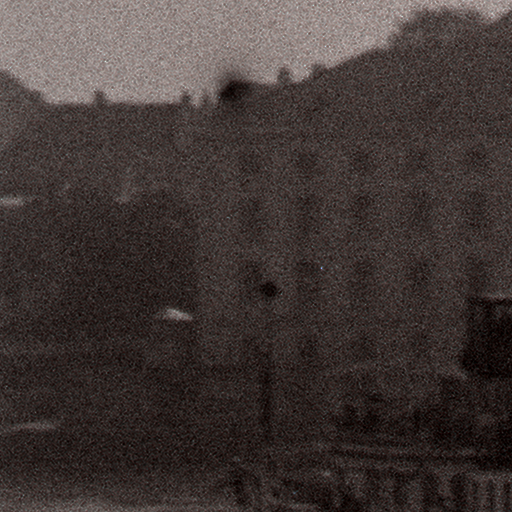
\includegraphics[width=.17\linewidth]{results_single/1000iter_early_combine/cnn_tests/cnn_tests3/input.png} & 
  		\setlength{\fboxrule}{0.5pt}
        \setlength{\fboxsep}{0pt}
        \framebox{\includegraphics[width=.17\linewidth, decodearray={1 0 1 0 1 0}]{results_single/1000iter_early_combine/cnn_tests/cnn_tests3/GT_mask.png}}& 
        \setlength{\fboxrule}{0.5pt}
        \setlength{\fboxsep}{0pt}
        \framebox{\includegraphics[width=.17\linewidth, decodearray={1 0 1 0 1 0}]{results_single/1000iter_early_combine/cnn_tests/cnn_tests3/pred_mask_TH.png}}&
        \setlength{\fboxrule}{0.5pt}
        \setlength{\fboxsep}{0pt}
         \framebox{\includegraphics[width=.17\linewidth, decodearray={1 0 1 0 1 0}]{results_single/1000iter_unet/cnn_tests/cnn_tests3/pred_mask_TH.png}} & 
        \setlength{\fboxrule}{0.5pt}
        \setlength{\fboxsep}{0pt}
        \framebox{\includegraphics[width=.17\linewidth, decodearray={1 0 1 0 1 0}]{results_single/1000iter_densenet/cnn_tests/cnn_tests3/pred_mask_TH.png}}\\
 \includegraphics[width=.17\linewidth]{results_single/1000iter_early_combine/cnn_tests/cnn_tests5/input.png} & 
 		\setlength{\fboxrule}{0.5pt}
        \setlength{\fboxsep}{0pt}
 		\framebox{\includegraphics[width=.17\linewidth, decodearray={1 0 1 0 1 0}]{results_single/1000iter_early_combine/cnn_tests/cnn_tests5/GT_mask.png}}&
 		\setlength{\fboxrule}{0.5pt}
        \setlength{\fboxsep}{0pt}
        \framebox{\includegraphics[width=.17\linewidth, decodearray={1 0 1 0 1 0}]{results_single/1000iter_early_combine/cnn_tests/cnn_tests5/pred_mask_TH.png}}&
        \setlength{\fboxrule}{0.5pt}
        \setlength{\fboxsep}{0pt}
        \framebox{\includegraphics[width=.17\linewidth, decodearray={1 0 1 0 1 0}]{results_single/1000iter_unet/cnn_tests/cnn_tests5/pred_mask_TH.png}}&
        \setlength{\fboxrule}{0.5pt}
        \setlength{\fboxsep}{0pt}
        \framebox{\includegraphics[width=.17\linewidth, decodearray={1 0 1 0 1 0}]{results_single/1000iter_densenet/cnn_tests/cnn_tests5/pred_mask_TH.png}}\\
 (a) Input & (b) GT & (c) Simple & (d) U-Net & (e) Densenet
\end{tabular}

\captionof{figure}{Sample results of single image segmentation for Simple (Figure~\ref{fig:single_simple}), U-Net ((Figure~\ref{fig:single_unet}) and Densenet (Figure~\ref{fig:single_densenet}).}
\label{fig:resu_single}
\end{center}\end{table}



\subsubsection{Multiple Input Images}
\label{ssec:num532}
Following prior results, we decided to not evaluate the UNet-architecture (Figure~\ref{fig:flow_unet}) but rather work with the other approaches from Section~\ref{ssec:num32}.

In Figure~\ref{fig:resu_flow_test_acc} the accuracy results of the different architectures on the test set are illustrated. One can see that the Densenet Combined model performs best, closely followed by the Densenet, Bottleneck and Densenet Combined 2 approach. The Early and Late models perform the worst. 

\begin{figure}[H]
	\centering
	\includegraphics[width=.6\linewidth]{results_flow/Test_Accuracy_Comparision.png}
	\caption[figure]{Accuracy for the different image segmentation architectures, evaluated on the test set. For the accuracy higher values mean better results. The best results are achieved with the Densenet Combined approach (Figure~\ref{fig:flow_densenet_comb}).}
	\label{fig:resu_flow_test_acc}
\end{figure}


Figure~\ref{fig:resu_flow_sets_acc} shows the accuracy of the different architectures on the sub-categorized test sets: large area (Figure~\ref{fig:resu_flow_LA_acc}), small area (Figure~\ref{fig:resu_flow_SA_acc}), large flow (Figure~\ref{fig:resu_flow_LF_acc}) and small flow (Figure~\ref{fig:resu_flow_SF_acc}).

The overall best architecture, Densenet Combined, also performs well on each of the single sub-test sets. The Bottleneck model also performs well on each of these subsets. The overall poor performing Early model achieves great results on the small area test set. Whereas the Late model performs on each single test set poorly.

\begin{figure}[H]
	\centering
	\begin{subfigure}{.48\textwidth}
		\centering
		\includegraphics[width=\linewidth]{results_flow/Large_Area_Accuracy_Comparision.png}
		\caption[figure]{Large area test set}
		\label{fig:resu_flow_LA_acc}
	\end{subfigure}
	\begin{subfigure}{.48\textwidth}
		\centering
		\includegraphics[width=\linewidth]{results_flow/Small_Area_Accuracy_Comparision.png}
		\caption[figure]{Small area test set}
		\label{fig:resu_flow_SA_acc}
	\end{subfigure} \\
	\begin{subfigure}{.48\textwidth}
		\centering
		\includegraphics[width=\linewidth]{results_flow/Large_Flow_Accuracy_Comparision.png}
		\caption[figure]{Large flow test set}
		\label{fig:resu_flow_LF_acc}
	\end{subfigure}
	\begin{subfigure}{.48\textwidth}
		\centering
		\includegraphics[width=\linewidth]{results_flow/Small_Flow_Accuracy_Comparision.png}
		\caption[figure]{Small flow test set}
		\label{fig:resu_flow_SF_acc}
	\end{subfigure} 	
	\caption[figure]{Accuracy for the different image segmentation architectures, evaluated on the sub-categorized test sets.}
	\label{fig:resu_flow_sets_acc}
\end{figure}

Figures~\ref{fig:resu_flow1}~and~\ref{fig:resu_flow2} give an overview of estimated segmentation masks of the different architectures compared to the ground-truth masks.






\begin{table}[H]\begin{center}
 \setlength{\tabcolsep}{1pt}
\begin{tabular}{ c c c c c}
 %\multicolumn{}{|c|}{Country List} \\
 
\includegraphics[width=.17\linewidth]{results_flow/1000iter_early_combine_wd_do/cnn_tests_restore/cnn_tests0/input.png} & \setlength{\fboxrule}{0.5pt} \setlength{\fboxsep}{0pt} \framebox{\includegraphics[width=.17\linewidth, decodearray={1 0 1 0 1 0}]{results_flow/1000iter_early_combine_wd_do/cnn_tests_restore/cnn_tests0/GT_mask.png}} & \setlength{\fboxrule}{0.5pt} \setlength{\fboxsep}{0pt} \framebox{\includegraphics[width=.17\linewidth, decodearray={1 0 1 0 1 0}]{results_flow/1000iter_early_combine_wd_do/cnn_tests_restore/cnn_tests0/pred_mask_TH.png}} &\setlength{\fboxrule}{0.5pt} \setlength{\fboxsep}{0pt} \framebox{ \includegraphics[width=.17\linewidth, decodearray={1 0 1 0 1 0}]{results_flow/1000iter_late_combine_wd_do/cnn_tests_restore/cnn_tests0/pred_mask_TH.png}} & \setlength{\fboxrule}{0.5pt} \setlength{\fboxsep}{0pt} \framebox{\includegraphics[width=.17\linewidth, decodearray={1 0 1 0 1 0}]{results_flow/1000iter_densenet_wd_do/cnn_tests_restore/cnn_tests0/pred_mask_TH.png}} \\
 \includegraphics[width=.17\linewidth]{results_flow/1000iter_early_combine_wd_do/cnn_tests_restore/cnn_tests3/input.png} & \setlength{\fboxrule}{0.5pt} \setlength{\fboxsep}{0pt} \framebox{\includegraphics[width=.17\linewidth, decodearray={1 0 1 0 1 0}]{results_flow/1000iter_early_combine_wd_do/cnn_tests_restore/cnn_tests3/GT_mask.png}} & \setlength{\fboxrule}{0.5pt} \setlength{\fboxsep}{0pt} \framebox{\includegraphics[width=.17\linewidth, decodearray={1 0 1 0 1 0}]{results_flow/1000iter_early_combine_wd_do/cnn_tests_restore/cnn_tests3/pred_mask_TH.png}} & \setlength{\fboxrule}{0.5pt} \setlength{\fboxsep}{0pt} \framebox{\includegraphics[width=.17\linewidth, decodearray={1 0 1 0 1 0}]{results_flow/1000iter_late_combine_wd_do/cnn_tests_restore/cnn_tests3/pred_mask_TH.png}} & \setlength{\fboxrule}{0.5pt} \setlength{\fboxsep}{0pt} \framebox{\includegraphics[width=.17\linewidth, decodearray={1 0 1 0 1 0}]{results_flow/1000iter_densenet_wd_do/cnn_tests_restore/cnn_tests3/pred_mask_TH.png}} \\
 \includegraphics[width=.17\linewidth]{results_flow/1000iter_early_combine_wd_do/cnn_tests_restore/cnn_tests5/input.png} & \setlength{\fboxrule}{0.5pt} \setlength{\fboxsep}{0pt} \framebox{\includegraphics[width=.17\linewidth, decodearray={1 0 1 0 1 0}]{results_flow/1000iter_early_combine_wd_do/cnn_tests_restore/cnn_tests5/GT_mask.png}} & \setlength{\fboxrule}{0.5pt} \setlength{\fboxsep}{0pt} \framebox{\includegraphics[width=.17\linewidth, decodearray={1 0 1 0 1 0}]{results_flow/1000iter_early_combine_wd_do/cnn_tests_restore/cnn_tests5/pred_mask_TH.png}} & \setlength{\fboxrule}{0.5pt} \setlength{\fboxsep}{0pt} \framebox{\includegraphics[width=.17\linewidth, decodearray={1 0 1 0 1 0}]{results_flow/1000iter_late_combine_wd_do/cnn_tests_restore/cnn_tests5/pred_mask_TH.png}} & \setlength{\fboxrule}{0.5pt} \setlength{\fboxsep}{0pt} \framebox{\includegraphics[width=.17\linewidth, decodearray={1 0 1 0 1 0}]{results_flow/1000iter_densenet_wd_do/cnn_tests_restore/cnn_tests5/pred_mask_TH.png}} \\
 (a) Input & (b) GT & (c) Early & (d) Late & (e) Densenet
\end{tabular}

\captionof{figure}{Sample results 1 of image segmentation using additional information for Early (Figure~\ref{fig:flow_early_combine}), Late (Figure~\ref{fig:flow_late_combine}) and Densenet (Figure~\ref{fig:flow_densenet}).}

%\caption{Comparison of thermal efficiency of Present study with O. Kaska []}
\label{fig:resu_flow1}
\end{center}\end{table}

\begin{table}[H]\begin{center}
 \setlength{\tabcolsep}{1pt}
\begin{tabular}{c c c c c}
 %\multicolumn{}{|c|}{Country List} \\
 
 \includegraphics[width=.17\linewidth]{results_flow/1000iter_densenet_comb_wd_do/cnn_tests_restore/cnn_tests0/input.png} & \setlength{\fboxrule}{0.5pt} \setlength{\fboxsep}{0pt} \framebox{\includegraphics[width=.17\linewidth, decodearray={1 0 1 0 1 0}]{results_flow/1000iter_densenet_comb_wd_do/cnn_tests_restore/cnn_tests0/GT_mask.png}} & \setlength{\fboxrule}{0.5pt} \setlength{\fboxsep}{0pt} \framebox{\includegraphics[width=.17\linewidth, decodearray={1 0 1 0 1 0}]{results_flow/1000iter_densenet_comb_wd_do/cnn_tests_restore/cnn_tests0/pred_mask_TH.png}} & \setlength{\fboxrule}{0.5pt} \setlength{\fboxsep}{0pt} \framebox{\includegraphics[width=.17\linewidth, decodearray={1 0 1 0 1 0}]{results_flow/1000iter_bottleneck_wd_do/cnn_tests_restore/cnn_tests0/pred_mask_TH.png}} & \setlength{\fboxrule}{0.5pt} \setlength{\fboxsep}{0pt} \framebox{\includegraphics[width=.17\linewidth, decodearray={1 0 1 0 1 0}]{results_flow/1000iter_densenet_comb2_wd_do/cnn_tests_restore/cnn_tests0/pred_mask_TH.png}} \\
 \includegraphics[width=.17\linewidth]{results_flow/1000iter_densenet_comb_wd_do/cnn_tests_restore/cnn_tests3/input.png} & \setlength{\fboxrule}{0.5pt} \setlength{\fboxsep}{0pt} \framebox{\includegraphics[width=.17\linewidth, decodearray={1 0 1 0 1 0}]{results_flow/1000iter_densenet_comb_wd_do/cnn_tests_restore/cnn_tests3/GT_mask.png}} & \setlength{\fboxrule}{0.5pt} \setlength{\fboxsep}{0pt} \framebox{\includegraphics[width=.17\linewidth, decodearray={1 0 1 0 1 0}]{results_flow/1000iter_densenet_comb_wd_do/cnn_tests_restore/cnn_tests3/pred_mask_TH.png}} & \setlength{\fboxrule}{0.5pt} \setlength{\fboxsep}{0pt} \framebox{\includegraphics[width=.17\linewidth, decodearray={1 0 1 0 1 0}]{results_flow/1000iter_bottleneck_wd_do/cnn_tests_restore/cnn_tests3/pred_mask_TH.png}} & \setlength{\fboxrule}{0.5pt} \setlength{\fboxsep}{0pt} \framebox{\includegraphics[width=.17\linewidth, decodearray={1 0 1 0 1 0}]{results_flow/1000iter_densenet_comb2_wd_do/cnn_tests_restore/cnn_tests3/pred_mask_TH.png}} \\
 \includegraphics[width=.17\linewidth]{results_flow/1000iter_densenet_comb_wd_do/cnn_tests_restore/cnn_tests5/input.png} & \setlength{\fboxrule}{0.5pt} \setlength{\fboxsep}{0pt} \framebox{\includegraphics[width=.17\linewidth, decodearray={1 0 1 0 1 0}]{results_flow/1000iter_densenet_comb_wd_do/cnn_tests_restore/cnn_tests5/GT_mask.png}} & \setlength{\fboxrule}{0.5pt} \setlength{\fboxsep}{0pt} \framebox{\includegraphics[width=.17\linewidth, decodearray={1 0 1 0 1 0}]{results_flow/1000iter_densenet_comb_wd_do/cnn_tests_restore/cnn_tests5/pred_mask_TH.png}} & \setlength{\fboxrule}{0.5pt} \setlength{\fboxsep}{0pt} \framebox{\includegraphics[width=.17\linewidth, decodearray={1 0 1 0 1 0}]{results_flow/1000iter_bottleneck_wd_do/cnn_tests_restore/cnn_tests5/pred_mask_TH.png}} & \setlength{\fboxrule}{0.5pt} \setlength{\fboxsep}{0pt} \framebox{\includegraphics[width=.17\linewidth, decodearray={1 0 1 0 1 0}]{results_flow/1000iter_densenet_comb2_wd_do/cnn_tests_restore/cnn_tests5/pred_mask_TH.png}} \\
 (a) Input & (b) GT & (c) \makecell{Densenet \\ Combined} & (d) Bottleneck & (e) \makecell{Densenet \\ Combined 2}
\end{tabular}

\captionof{figure}{Sample results 2 of image segmentation using additional information for Densenet Combined (Figure~\ref{fig:flow_densenet_comb}), Bottleneck (Figure~\ref{fig:flow_bottleneck}) and Densenet Combined 2 (Figure~\ref{fig:flow_densenet_comb2}).}

%\caption{Comparison of thermal efficiency of Present study with O. Kaska []}
\label{fig:resu_flow2}
\end{center}\end{table}

The first example in Figure~\ref{fig:resu_flow1}~and~\ref{fig:resu_flow2} show the impurity segmentation for a sequence with few motion. One can see that the resulting segmentation masks are quite similar compared to the ground-truth.  

The last two rows in Figure~\ref{fig:resu_flow1}~and~\ref{fig:resu_flow2} visualize sample results for sequences with large optical flow. In one example there is a large hand movement, whereas in the other there is a large vertical camera motion. The resulting segmentation masks in these examples is not able to estimate the impurities. The large optical flow has a too large impact into the impurity detection.

\subsubsection{Multiple Warped Input Images}
\label{ssec:num533}
As already mentioned we trained all the CNN architectures once for the warped image instances and once without warping to see if there is a difference.
The results in Figure~\ref{fig:resu_warp_test_acc} suggest that by using warped instances for the previous and next images we can improve the segmentation of the impurities. The best results were achieved with the bottleneck architecture and warped image instances. Interestingly, for all variants of the densenet structure, training with unwarped data achieves better results.

Figure~\ref{fig:resu_warp1}~and~\ref{fig:resu_warp2} show results for architectures trained on the warped instances for previous and next images. Figure~\ref{fig:resu_warp3}~and~\ref{fig:resu_warp4} show results for the same sequences but with unwarped previous and next images. The first and second example are sequences with low optical flow. For these examples both training methods achieve equal good results. The last example has a large optical flow and the training on the warped image instances achieves better results.

\begin{figure}[H]
	\centering
	\includegraphics[width=.6\linewidth]{results_warp/Test_Accuracy_Comparision.png}
	\caption[figure]{Accuracy for the different image segmentation architectures for warped and unwarped image instances. For the accuracy higher values mean better results. The best results are achieved with the Bottleneck approach (Figure~\ref{fig:flow_bottleneck}) and warped previous and next images.}
	\label{fig:resu_warp_test_acc}
\end{figure}


\begin{table}[H]\begin{center}
 \setlength{\tabcolsep}{1pt}
\begin{tabular}{c c c c c}
 %\multicolumn{}{|c|}{Country List} \\

 \includegraphics[width=.17\linewidth]{results_warp/results/results_early/cnn_tests_restore/cnn_tests1/input.png} & \setlength{\fboxrule}{0.5pt} \setlength{\fboxsep}{0pt} \framebox{\includegraphics[width=.17\linewidth, decodearray={1 0 1 0 1 0}]{results_warp/results/results_early/cnn_tests_restore/cnn_tests1/GT_mask.png}} & \setlength{\fboxrule}{0.5pt} \setlength{\fboxsep}{0pt} \framebox{\includegraphics[width=.17\linewidth, decodearray={1 0 1 0 1 0}]{results_warp/results/results_early/cnn_tests_restore/cnn_tests1/pred_mask_TH.png}} & \setlength{\fboxrule}{0.5pt} \setlength{\fboxsep}{0pt} \framebox{\includegraphics[width=.17\linewidth, decodearray={1 0 1 0 1 0}]{results_warp/results/results_late/cnn_tests_restore/cnn_tests1/pred_mask_TH.png}} & \setlength{\fboxrule}{0.5pt} \setlength{\fboxsep}{0pt} \framebox{\includegraphics[width=.17\linewidth, decodearray={1 0 1 0 1 0}]{results_warp/results/results_densenet/cnn_tests_restore/cnn_tests1/pred_mask_TH.png}} \\
 \includegraphics[width=.17\linewidth]{results_warp/results/results_early/cnn_tests_restore/cnn_tests5/input.png} & \setlength{\fboxrule}{0.5pt} \setlength{\fboxsep}{0pt} \framebox{\includegraphics[width=.17\linewidth, decodearray={1 0 1 0 1 0}]{results_warp/results/results_early/cnn_tests_restore/cnn_tests5/GT_mask.png}} & \setlength{\fboxrule}{0.5pt} \setlength{\fboxsep}{0pt} \framebox{\includegraphics[width=.17\linewidth, decodearray={1 0 1 0 1 0}]{results_warp/results/results_early/cnn_tests_restore/cnn_tests5/pred_mask_TH.png}} & \setlength{\fboxrule}{0.5pt} \setlength{\fboxsep}{0pt} \framebox{\includegraphics[width=.17\linewidth, decodearray={1 0 1 0 1 0}]{results_warp/results/results_late/cnn_tests_restore/cnn_tests5/pred_mask_TH.png}} & \setlength{\fboxrule}{0.5pt} \setlength{\fboxsep}{0pt} \framebox{\includegraphics[width=.17\linewidth, decodearray={1 0 1 0 1 0}]{results_warp/results/results_densenet/cnn_tests_restore/cnn_tests5/pred_mask_TH.png}} \\
 \includegraphics[width=.17\linewidth]{results_warp/results/results_early/cnn_tests_restore/cnn_tests9/input.png} & \setlength{\fboxrule}{0.5pt} \setlength{\fboxsep}{0pt} \framebox{\includegraphics[width=.17\linewidth, decodearray={1 0 1 0 1 0}]{results_warp/results/results_early/cnn_tests_restore/cnn_tests9/GT_mask.png}} & \setlength{\fboxrule}{0.5pt} \setlength{\fboxsep}{0pt} \framebox{\includegraphics[width=.17\linewidth, decodearray={1 0 1 0 1 0}]{results_warp/results/results_early/cnn_tests_restore/cnn_tests9/pred_mask_TH.png}} & \setlength{\fboxrule}{0.5pt} \setlength{\fboxsep}{0pt} \framebox{\includegraphics[width=.17\linewidth, decodearray={1 0 1 0 1 0}]{results_warp/results/results_late/cnn_tests_restore/cnn_tests9/pred_mask_TH.png}} & \setlength{\fboxrule}{0.5pt} \setlength{\fboxsep}{0pt} \framebox{\includegraphics[width=.17\linewidth, decodearray={1 0 1 0 1 0}]{results_warp/results/results_densenet/cnn_tests_restore/cnn_tests9/pred_mask_TH.png}} \\
 (a) Input & (b) GT & (c) Early & (d) Late & (e) Densenet
\end{tabular}

\captionof{figure}{Sample results 1 of image segmentation using additional warped information for Early (Figure~\ref{fig:flow_early_combine}), Late (Figure~\ref{fig:flow_late_combine}) and Densenet (Figure~\ref{fig:flow_densenet}).}

%\caption{Comparison of thermal efficiency of Present study with O. Kaska []}
\label{fig:resu_warp1}
\end{center}\end{table}

\begin{table}[H]\begin{center}
 \setlength{\tabcolsep}{1pt}
\begin{tabular}{c c c c c}
 %\multicolumn{}{|c|}{Country List} \\
 
 
 \includegraphics[width=.17\linewidth]{results_warp/results/results_densenet_comb/cnn_tests_restore/cnn_tests1/input.png} & \setlength{\fboxrule}{0.5pt} \setlength{\fboxsep}{0pt} \framebox{\includegraphics[width=.17\linewidth, decodearray={1 0 1 0 1 0}]{results_warp/results/results_densenet_comb/cnn_tests_restore/cnn_tests1/GT_mask.png}} & \setlength{\fboxrule}{0.5pt} \setlength{\fboxsep}{0pt} \framebox{\includegraphics[width=.17\linewidth, decodearray={1 0 1 0 1 0}]{results_warp/results/results_densenet_comb/cnn_tests_restore/cnn_tests1/pred_mask_TH.png}} & \setlength{\fboxrule}{0.5pt} \setlength{\fboxsep}{0pt} \framebox{\includegraphics[width=.17\linewidth, decodearray={1 0 1 0 1 0}]{results_warp/results/results_bottleneck/cnn_tests_restore/cnn_tests1/pred_mask_TH.png}} & \setlength{\fboxrule}{0.5pt} \setlength{\fboxsep}{0pt} \framebox{\includegraphics[width=.17\linewidth, decodearray={1 0 1 0 1 0}]{results_warp/results/results_densenet_comb2/cnn_tests_restore/cnn_tests1/pred_mask_TH.png}} 
 \\
 \includegraphics[width=.17\linewidth]{results_warp/results/results_densenet_comb/cnn_tests_restore/cnn_tests5/input.png} & \setlength{\fboxrule}{0.5pt} \setlength{\fboxsep}{0pt} \framebox{\includegraphics[width=.17\linewidth, decodearray={1 0 1 0 1 0}]{results_warp/results/results_densenet_comb/cnn_tests_restore/cnn_tests5/GT_mask.png}} & \setlength{\fboxrule}{0.5pt} \setlength{\fboxsep}{0pt} \framebox{\includegraphics[width=.17\linewidth, decodearray={1 0 1 0 1 0}]{results_warp/results/results_densenet_comb/cnn_tests_restore/cnn_tests5/pred_mask_TH.png}} & \setlength{\fboxrule}{0.5pt} \setlength{\fboxsep}{0pt} \framebox{\includegraphics[width=.17\linewidth, decodearray={1 0 1 0 1 0}]{results_warp/results/results_bottleneck/cnn_tests_restore/cnn_tests5/pred_mask_TH.png}} & \setlength{\fboxrule}{0.5pt} \setlength{\fboxsep}{0pt} \framebox{\includegraphics[width=.17\linewidth, decodearray={1 0 1 0 1 0}]{results_warp/results/results_densenet_comb2/cnn_tests_restore/cnn_tests5/pred_mask_TH.png}} \\
 \includegraphics[width=.17\linewidth]{results_warp/results/results_densenet_comb/cnn_tests_restore/cnn_tests9/input.png} & \setlength{\fboxrule}{0.5pt} \setlength{\fboxsep}{0pt} \framebox{\includegraphics[width=.17\linewidth, decodearray={1 0 1 0 1 0}]{results_warp/results/results_densenet_comb/cnn_tests_restore/cnn_tests9/GT_mask.png}} & \setlength{\fboxrule}{0.5pt} \setlength{\fboxsep}{0pt} \framebox{\includegraphics[width=.17\linewidth, decodearray={1 0 1 0 1 0}]{results_warp/results/results_densenet_comb/cnn_tests_restore/cnn_tests9/pred_mask_TH.png}} & \setlength{\fboxrule}{0.5pt} \setlength{\fboxsep}{0pt} \framebox{\includegraphics[width=.17\linewidth, decodearray={1 0 1 0 1 0}]{results_warp/results/results_bottleneck/cnn_tests_restore/cnn_tests9/pred_mask_TH.png}} & \setlength{\fboxrule}{0.5pt} \setlength{\fboxsep}{0pt} \framebox{\includegraphics[width=.17\linewidth, decodearray={1 0 1 0 1 0}]{results_warp/results/results_densenet_comb2/cnn_tests_restore/cnn_tests9/pred_mask_TH.png}} \\
 (a) Input & (b) GT & (c) \makecell{Densenet \\ Combined} & (d) Bottleneck & (e) \makecell{Densenet \\ Combined 2}
\end{tabular}

\captionof{figure}{Sample results 2 of image segmentation using additional warped information for Densenet Combined (Figure~\ref{fig:flow_densenet_comb}), Bottleneck (Figure~\ref{fig:flow_bottleneck}) and Densenet Combined 2 (Figure~\ref{fig:flow_densenet_comb2}).}

%\caption{Comparison of thermal efficiency of Present study with O. Kaska []}
\label{fig:resu_warp2}
\end{center}\end{table}

\begin{table}[H]\begin{center}
 \setlength{\tabcolsep}{1pt}
\begin{tabular}{c c c c c}
 %\multicolumn{}{|c|}{Country List} \\
 

 \includegraphics[width=.17\linewidth]{results_warp/results_not/results_early/cnn_tests_restore/cnn_tests1/input.png} & \setlength{\fboxrule}{0.5pt} \setlength{\fboxsep}{0pt} \framebox{\includegraphics[width=.17\linewidth, decodearray={1 0 1 0 1 0}]{results_warp/results_not/results_early/cnn_tests_restore/cnn_tests1/GT_mask.png}} & \setlength{\fboxrule}{0.5pt} \setlength{\fboxsep}{0pt} \framebox{\includegraphics[width=.17\linewidth, decodearray={1 0 1 0 1 0}]{results_warp/results_not/results_early/cnn_tests_restore/cnn_tests1/pred_mask_TH.png}} & \setlength{\fboxrule}{0.5pt} \setlength{\fboxsep}{0pt} \framebox{\includegraphics[width=.17\linewidth, decodearray={1 0 1 0 1 0}]{results_warp/results_not/results_late/cnn_tests_restore/cnn_tests1/pred_mask_TH.png}} & \setlength{\fboxrule}{0.5pt} \setlength{\fboxsep}{0pt} \framebox{\includegraphics[width=.17\linewidth, decodearray={1 0 1 0 1 0}]{results_warp/results_not/results_densenet/cnn_tests_restore/cnn_tests1/pred_mask_TH.png}} 
 \\
 \includegraphics[width=.17\linewidth]{results_warp/results_not/results_early/cnn_tests_restore/cnn_tests5/input.png} & \setlength{\fboxrule}{0.5pt} \setlength{\fboxsep}{0pt} \framebox{\includegraphics[width=.17\linewidth, decodearray={1 0 1 0 1 0}]{results_warp/results_not/results_early/cnn_tests_restore/cnn_tests5/GT_mask.png}} & \setlength{\fboxrule}{0.5pt} \setlength{\fboxsep}{0pt} \framebox{\includegraphics[width=.17\linewidth, decodearray={1 0 1 0 1 0}]{results_warp/results_not/results_early/cnn_tests_restore/cnn_tests5/pred_mask_TH.png}} & \setlength{\fboxrule}{0.5pt} \setlength{\fboxsep}{0pt} \framebox{\includegraphics[width=.17\linewidth, decodearray={1 0 1 0 1 0}]{results_warp/results_not/results_late/cnn_tests_restore/cnn_tests5/pred_mask_TH.png}} & \setlength{\fboxrule}{0.5pt} \setlength{\fboxsep}{0pt} \framebox{\includegraphics[width=.17\linewidth, decodearray={1 0 1 0 1 0}]{results_warp/results_not/results_densenet/cnn_tests_restore/cnn_tests5/pred_mask_TH.png}} 
 \\
 \includegraphics[width=.17\linewidth]{results_warp/results_not/results_early/cnn_tests_restore/cnn_tests9/input.png} & \setlength{\fboxrule}{0.5pt} \setlength{\fboxsep}{0pt} \framebox{\includegraphics[width=.17\linewidth, decodearray={1 0 1 0 1 0}]{results_warp/results_not/results_early/cnn_tests_restore/cnn_tests9/GT_mask.png}} & \setlength{\fboxrule}{0.5pt} \setlength{\fboxsep}{0pt} \framebox{\includegraphics[width=.17\linewidth, decodearray={1 0 1 0 1 0}]{results_warp/results_not/results_early/cnn_tests_restore/cnn_tests9/pred_mask_TH.png}} & \setlength{\fboxrule}{0.5pt} \setlength{\fboxsep}{0pt} \framebox{\includegraphics[width=.17\linewidth, decodearray={1 0 1 0 1 0}]{results_warp/results_not/results_late/cnn_tests_restore/cnn_tests9/pred_mask_TH.png}} & \setlength{\fboxrule}{0.5pt} \setlength{\fboxsep}{0pt} \framebox{\includegraphics[width=.17\linewidth, decodearray={1 0 1 0 1 0}]{results_warp/results_not/results_densenet/cnn_tests_restore/cnn_tests9/pred_mask_TH.png}} \\
 (a) Input & (b) GT & (c) Early & (d) Late & (e) Densenet
\end{tabular}

\captionof{figure}{Sample results 1 of image segmentation using additional unwarped information for Early (Figure~\ref{fig:flow_early_combine}), Late (Figure~\ref{fig:flow_late_combine}) and Densenet (Figure~\ref{fig:flow_densenet}).}

%\caption{Comparison of thermal efficiency of Present study with O. Kaska []}
\label{fig:resu_warp3}
\end{center}\end{table}

\begin{table}[H]\begin{center}
 \setlength{\tabcolsep}{1pt}
\begin{tabular}{c c c c c}
 %\multicolumn{}{|c|}{Country List} \\
 
 \includegraphics[width=.17\linewidth]{results_warp/results_not/results_densenet_comb/cnn_tests_restore/cnn_tests1/input.png} & \setlength{\fboxrule}{0.5pt} \setlength{\fboxsep}{0pt} \framebox{\includegraphics[width=.17\linewidth, decodearray={1 0 1 0 1 0}]{results_warp/results_not/results_densenet_comb/cnn_tests_restore/cnn_tests1/GT_mask.png}} & \setlength{\fboxrule}{0.5pt} \setlength{\fboxsep}{0pt} \framebox{\includegraphics[width=.17\linewidth, decodearray={1 0 1 0 1 0}]{results_warp/results_not/results_densenet_comb/cnn_tests_restore/cnn_tests1/pred_mask_TH.png}} & \setlength{\fboxrule}{0.5pt} \setlength{\fboxsep}{0pt} \framebox{\includegraphics[width=.17\linewidth, decodearray={1 0 1 0 1 0}]{results_warp/results_not/results_bottleneck/cnn_tests_restore/cnn_tests1/pred_mask_TH.png}} & \setlength{\fboxrule}{0.5pt} \setlength{\fboxsep}{0pt} \framebox{\includegraphics[width=.17\linewidth, decodearray={1 0 1 0 1 0}]{results_warp/results_not/results_densenet_comb2/cnn_tests_restore/cnn_tests1/pred_mask_TH.png}} \\
 \includegraphics[width=.17\linewidth]{results_warp/results_not/results_densenet_comb/cnn_tests_restore/cnn_tests5/input.png} & \setlength{\fboxrule}{0.5pt} \setlength{\fboxsep}{0pt} \framebox{\includegraphics[width=.17\linewidth, decodearray={1 0 1 0 1 0}]{results_warp/results_not/results_densenet_comb/cnn_tests_restore/cnn_tests5/GT_mask.png}} &\setlength{\fboxrule}{0.5pt} \setlength{\fboxsep}{0pt} \framebox{ \includegraphics[width=.17\linewidth, decodearray={1 0 1 0 1 0}]{results_warp/results_not/results_densenet_comb/cnn_tests_restore/cnn_tests5/pred_mask_TH.png}} & \setlength{\fboxrule}{0.5pt} \setlength{\fboxsep}{0pt} \framebox{\includegraphics[width=.17\linewidth, decodearray={1 0 1 0 1 0}]{results_warp/results_not/results_bottleneck/cnn_tests_restore/cnn_tests5/pred_mask_TH.png}} & \setlength{\fboxrule}{0.5pt} \setlength{\fboxsep}{0pt} \framebox{\includegraphics[width=.17\linewidth, decodearray={1 0 1 0 1 0}]{results_warp/results_not/results_densenet_comb2/cnn_tests_restore/cnn_tests5/pred_mask_TH.png}} \\
 \includegraphics[width=.17\linewidth]{results_warp/results_not/results_densenet_comb/cnn_tests_restore/cnn_tests9/input.png} & \setlength{\fboxrule}{0.5pt} \setlength{\fboxsep}{0pt} \framebox{\includegraphics[width=.17\linewidth, decodearray={1 0 1 0 1 0}]{results_warp/results_not/results_densenet_comb/cnn_tests_restore/cnn_tests9/GT_mask.png}} & \setlength{\fboxrule}{0.5pt} \setlength{\fboxsep}{0pt} \framebox{\includegraphics[width=.17\linewidth, decodearray={1 0 1 0 1 0}]{results_warp/results_not/results_densenet_comb/cnn_tests_restore/cnn_tests9/pred_mask_TH.png}} & \setlength{\fboxrule}{0.5pt} \setlength{\fboxsep}{0pt} \framebox{\includegraphics[width=.17\linewidth, decodearray={1 0 1 0 1 0}]{results_warp/results_not/results_bottleneck/cnn_tests_restore/cnn_tests9/pred_mask_TH.png}} & \setlength{\fboxrule}{0.5pt} \setlength{\fboxsep}{0pt} \framebox{\includegraphics[width=.17\linewidth, decodearray={1 0 1 0 1 0}]{results_warp/results_not/results_densenet_comb2/cnn_tests_restore/cnn_tests9/pred_mask_TH.png}} \\
 (a) Input & (b) GT & (c) \makecell{Densenet \\ Combined} & (d) Bottleneck & (e) \makecell{Densenet \\ Combined 2}
\end{tabular}

\captionof{figure}{Sample results 2 of image segmentation using additional unwarped information for Densenet Combined (Figure~\ref{fig:flow_densenet_comb}), Bottleneck (Figure~\ref{fig:flow_bottleneck}) and Densenet Combined 2 (Figure~\ref{fig:flow_densenet_comb2}).}

%\caption{Comparison of thermal efficiency of Present study with O. Kaska []}
\label{fig:resu_warp4}
\end{center}\end{table}



\subsection{Results for Image In-painting}
\label{ssec:num54}

In the following Sections we list the results of image in-painting using the generated segmentation mask (Section~\ref{sssec:num541}) from the Densenet Combined model and in Section~\ref{sssec:num542} we list the results of image in-painting without a segmentation mask.

\subsubsection{With Segmentation Mask}
\label{sssec:num541}

Figure~\ref{fig:resu_pm} gives an overview of the results of different image in-painting approaches. The first three examples are sequences with few optical flow. For this examples the predicted segmentation masks are of good quality and therefore the the image in-painting achieves visually pleasing results. 
The last two examples have more optical flow. For the sequence with the building, there is a vertical motion of the camera and for the other sequence, there is a strong movement of the hand. As there is a large optical flow, the predicted segmentation mask is bad and therefore the image in-painting performs also bad compared to the ground truth.

One can see that the Densenet Copy approach achieves the visual most appealing image in-painting results followed by the Densenet Add. The Perona-Malik method has the visual worst results.

\begin{table}[H]\begin{center}
 \setlength{\tabcolsep}{2pt}
\begin{tabular}{c c c c c c}
 %\multicolumn{}{|c|}{Country List} \\
 
 \includegraphics[width=.15\linewidth]{results_painting_pred_masks/results_densenet_comb_predict_masks/cnn_tests_restore/cnn_tests0/input.png} & \setlength{\fboxrule}{0.5pt}
        \setlength{\fboxsep}{0pt}\framebox{\includegraphics[width=.15\linewidth, decodearray={1 0 1 0 1 0}]{results_painting_pred_masks/results_densenet_comb_predict_masks/cnn_tests_restore/cnn_tests0/GT_mask.png}} & \includegraphics[width=.15\linewidth]{results_painting_pred_masks/results_densenet_comb_predict_masks/cnn_tests_restore/cnn_tests0/GT_out.png}& \includegraphics[width=.15\linewidth]{results_painting_pred_masks/results_densenet_predict_masks/cnn_tests_restore/cnn_tests0/pred_out.png} & \includegraphics[width=.15\linewidth]{results_painting_pred_masks/results_densenet_comb_predict_masks/cnn_tests_restore/cnn_tests0/pred_out.png} & \includegraphics[width=.15\linewidth]{results_painting_pred_masks/results_pm_predict_masks/results0/res_diffusion.png} \\
       \includegraphics[width=.15\linewidth]{results_painting_pred_masks/results_densenet_comb_predict_masks/cnn_tests_restore/cnn_tests7/input.png} & \setlength{\fboxrule}{0.5pt}
        \setlength{\fboxsep}{0pt}\framebox{\includegraphics[width=.15\linewidth, decodearray={1 0 1 0 1 0}]{results_painting_pred_masks/results_densenet_comb_predict_masks/cnn_tests_restore/cnn_tests7/GT_mask.png}} & \includegraphics[width=.15\linewidth]{results_painting_pred_masks/results_densenet_comb_predict_masks/cnn_tests_restore/cnn_tests7/GT_out.png}& \includegraphics[width=.15\linewidth]{results_painting_pred_masks/results_densenet_predict_masks/cnn_tests_restore/cnn_tests7/pred_out.png} & \includegraphics[width=.15\linewidth]{results_painting_pred_masks/results_densenet_comb_predict_masks/cnn_tests_restore/cnn_tests7/pred_out.png} & \includegraphics[width=.15\linewidth]{results_painting_pred_masks/results_pm_predict_masks/results7/res_diffusion.png} \\
        \includegraphics[width=.15\linewidth]{results_painting_pred_masks/results_densenet_comb_predict_masks/cnn_tests_restore/cnn_tests9/input.png} & \setlength{\fboxrule}{0.5pt}
        \setlength{\fboxsep}{0pt}\framebox{\includegraphics[width=.15\linewidth, decodearray={1 0 1 0 1 0}]{results_painting_pred_masks/results_densenet_comb_predict_masks/cnn_tests_restore/cnn_tests9/GT_mask.png}} & \includegraphics[width=.15\linewidth]{results_painting_pred_masks/results_densenet_comb_predict_masks/cnn_tests_restore/cnn_tests9/GT_out.png}& \includegraphics[width=.15\linewidth]{results_painting_pred_masks/results_densenet_predict_masks/cnn_tests_restore/cnn_tests9/pred_out.png} &
 \includegraphics[width=.15\linewidth]{results_painting_pred_masks/results_densenet_comb_predict_masks/cnn_tests_restore/cnn_tests9/pred_out.png} & \includegraphics[width=.15\linewidth]{results_painting_pred_masks/results_pm_predict_masks/results9/res_diffusion.png} \\
     \includegraphics[width=.15\linewidth]{results_painting_pred_masks/results_densenet_comb_predict_masks/cnn_tests_restore/cnn_tests3/input.png} & \setlength{\fboxrule}{0.5pt}
        \setlength{\fboxsep}{0pt}\framebox{\includegraphics[width=.15\linewidth, decodearray={1 0 1 0 1 0}]{results_painting_pred_masks/results_densenet_comb_predict_masks/cnn_tests_restore/cnn_tests3/GT_mask.png}} & \includegraphics[width=.15\linewidth]{results_painting_pred_masks/results_densenet_comb_predict_masks/cnn_tests_restore/cnn_tests3/GT_out.png}& \includegraphics[width=.15\linewidth]{results_painting_pred_masks/results_densenet_predict_masks/cnn_tests_restore/cnn_tests3/pred_out.png} & \includegraphics[width=.15\linewidth]{results_painting_pred_masks/results_densenet_comb_predict_masks/cnn_tests_restore/cnn_tests3/pred_out.png} &\includegraphics[width=.15\linewidth]{results_painting_pred_masks/results_pm_predict_masks/results3/res_diffusion.png} \\
     \includegraphics[width=.15\linewidth]{results_painting_pred_masks/results_densenet_comb_predict_masks/cnn_tests_restore/cnn_tests5/input.png} & \setlength{\fboxrule}{0.5pt}
        \setlength{\fboxsep}{0pt}\framebox{\includegraphics[width=.15\linewidth, decodearray={1 0 1 0 1 0}]{results_painting_pred_masks/results_densenet_comb_predict_masks/cnn_tests_restore/cnn_tests5/GT_mask.png}} & \includegraphics[width=.15\linewidth]{results_painting_pred_masks/results_densenet_comb_predict_masks/cnn_tests_restore/cnn_tests5/GT_out.png}& \includegraphics[width=.15\linewidth]{results_painting_pred_masks/results_densenet_predict_masks/cnn_tests_restore/cnn_tests5/pred_out.png} & \includegraphics[width=.15\linewidth]{results_painting_pred_masks/results_densenet_comb_predict_masks/cnn_tests_restore/cnn_tests5/pred_out.png} & \includegraphics[width=.15\linewidth]{results_painting_pred_masks/results_pm_predict_masks/results5/res_diffusion.png} \\
 (a) Input & (b) Mask & (c) GT & (d) \makecell{Densenet\\Copy} & (e) \makecell{Densenet\\Add} & (f) \makecell{Perona-\\Malik}
\end{tabular}

\captionof{figure}{Sample results of image in-painting with estimated segmentation mask for Densenet Copy (Figure~\ref{fig:paint_densenet}), Densenet Add (Figure~\ref{fig:paint_densenet2}) and Perona-Malik (Section~\ref{ssec:num42}).}
%\caption{Comparison of thermal efficiency of Present study with O. Kaska []}
\label{fig:resu_pm}
\end{center}\end{table}


\subsubsection{Without Segmentation Mask}
\label{sssec:num542}

Figure~\ref{fig:resu_pm2} gives an overview of the results of different image in-painting approaches without the use of a segmentation mask. The first three sequences have few optical flow. The image in-painting for these sequences works well compared to the ground truth. The last two sequences have more optical flow. For the sequence with the head, there is a horizontal motion, and in the last sequence there is strong motion of the ball. For these two sequences the image in-painting does not just correct the impurities but also adds some artifacts.

One can see that the Densenet Add approach, trained on a single image channel, achieves the visual most appealing image in-painting results. For the approaches trained on color images, the Densenet Add model performs better than the Densenet Combine Add model.

\begin{table}[H]\begin{center}
 \setlength{\tabcolsep}{1pt}
\begin{tabular}{c c c c c c}
 %\multicolumn{}{|c|}{Country List} \\
 
 
    \includegraphics[width=.15\linewidth]{results_painting_warp/inpai6/cnn_tests_restore/cnn_tests4/input.png} & \setlength{\fboxrule}{0.5pt}
        \setlength{\fboxsep}{0pt}\framebox{\includegraphics[width=.15\linewidth, decodearray={1 0 1 0 1 0}]{results_painting_warp/inpai6/cnn_tests_restore/cnn_tests4/GT_mask.png}} & \includegraphics[width=.15\linewidth]{results_painting_warp/inpai6/cnn_tests_restore/cnn_tests4/GT_out.png}& \includegraphics[width=.15\linewidth]{results_painting_warp/inpai5/cnn_tests_restore/cnn_tests4/pred_out.png} & \includegraphics[width=.15\linewidth]{results_painting_warp/inpai6/cnn_tests_restore/cnn_tests4/pred_out.png} &\includegraphics[width=.15\linewidth]{results_painting_warp/inpai7/cnn_tests_restore/cnn_tests4/pred_out.png} \\
     \includegraphics[width=.15\linewidth]{results_painting_warp/inpai6/cnn_tests_restore/cnn_tests8/input.png} & \setlength{\fboxrule}{0.5pt}
        \setlength{\fboxsep}{0pt}\framebox{\includegraphics[width=.15\linewidth, decodearray={1 0 1 0 1 0}]{results_painting_warp/inpai6/cnn_tests_restore/cnn_tests8/GT_mask.png}} & \includegraphics[width=.15\linewidth]{results_painting_warp/inpai6/cnn_tests_restore/cnn_tests8/GT_out.png}& \includegraphics[width=.15\linewidth]{results_painting_warp/inpai5/cnn_tests_restore/cnn_tests8/pred_out.png} & \includegraphics[width=.15\linewidth]{results_painting_warp/inpai6/cnn_tests_restore/cnn_tests8/pred_out.png} & \includegraphics[width=.15\linewidth]{results_painting_warp/inpai7/cnn_tests_restore/cnn_tests8/pred_out.png} \\
       \includegraphics[width=.15\linewidth]{results_painting_warp/inpai6/cnn_tests_restore/cnn_tests9/input.png} & \setlength{\fboxrule}{0.5pt}
        \setlength{\fboxsep}{0pt}\framebox{\includegraphics[width=.15\linewidth, decodearray={1 0 1 0 1 0}]{results_painting_warp/inpai6/cnn_tests_restore/cnn_tests9/GT_mask.png}} & \includegraphics[width=.15\linewidth]{results_painting_warp/inpai6/cnn_tests_restore/cnn_tests9/GT_out.png}& \includegraphics[width=.15\linewidth]{results_painting_warp/inpai5/cnn_tests_restore/cnn_tests9/pred_out.png} & \includegraphics[width=.15\linewidth]{results_painting_warp/inpai6/cnn_tests_restore/cnn_tests9/pred_out.png} & \includegraphics[width=.15\linewidth]{results_painting_warp/inpai7/cnn_tests_restore/cnn_tests9/pred_out.png} \\
        \includegraphics[width=.15\linewidth]{results_painting_warp/inpai6/cnn_tests_restore/cnn_tests1/input.png} & \setlength{\fboxrule}{0.5pt}
        \setlength{\fboxsep}{0pt}\framebox{\includegraphics[width=.15\linewidth, decodearray={1 0 1 0 1 0}]{results_painting_warp/inpai6/cnn_tests_restore/cnn_tests1/GT_mask.png}} & \includegraphics[width=.15\linewidth]{results_painting_warp/inpai6/cnn_tests_restore/cnn_tests1/GT_out.png}& \includegraphics[width=.15\linewidth]{results_painting_warp/inpai5/cnn_tests_restore/cnn_tests1/pred_out.png} & \includegraphics[width=.15\linewidth]{results_painting_warp/inpai6/cnn_tests_restore/cnn_tests1/pred_out.png} & \includegraphics[width=.15\linewidth]{results_painting_warp/inpai7/cnn_tests_restore/cnn_tests1/pred_out.png} \\
        \includegraphics[width=.15\linewidth]{results_painting_warp/inpai6/cnn_tests_restore/cnn_tests11/input.png} & \setlength{\fboxrule}{0.5pt}
        \setlength{\fboxsep}{0pt}\framebox{\includegraphics[width=.15\linewidth, decodearray={1 0 1 0 1 0}]{results_painting_warp/inpai6/cnn_tests_restore/cnn_tests11/GT_mask.png}} & \includegraphics[width=.15\linewidth]{results_painting_warp/inpai6/cnn_tests_restore/cnn_tests11/GT_out.png}& \includegraphics[width=.15\linewidth]{results_painting_warp/inpai5/cnn_tests_restore/cnn_tests11/pred_out.png} &
 \includegraphics[width=.15\linewidth]{results_painting_warp/inpai6/cnn_tests_restore/cnn_tests11/pred_out.png} & \includegraphics[width=.15\linewidth]{results_painting_warp/inpai7/cnn_tests_restore/cnn_tests11/pred_out.png} \\
 (a) Input & (b) GT-Mask & (c) GT & (d) \makecell{Densenet\\Add\\one channel} & (e) \makecell{Densenet\\Add\\color image} & (f) \makecell{Densenet\\Combine Add\\color image}
\end{tabular}

\captionof{figure}{Sample results of image in-painting without estimated segmentation mask for Densenet Add (Figure~\ref{fig:inpai5}) that was trained and tested on a single color channel, and the models trained and tested on color images: Densenet Add (Figure~\ref{fig:inpai6}) and Densenet Combine Add (Figure~\ref{fig:inpai7}).}
%\caption{Comparison of thermal efficiency of Present study with O. Kaska []}
\label{fig:resu_pm2}
\end{center}\end{table}

\newpage
\section{Conclusion}
\label{sec:num6}

We have introduced a deep learning method to perform image restoration. We showed that a two part approach, splitting into the detection of the impurities and the correction of them, is able to produce visually appealing results.\\

The impurity detection based on image segmentation as in Section~\ref{ssec:num32} works best with the Densenet Combined model (Figure~\ref{fig:flow_densenet_comb}). By investigating segmentation mask results (Figure~\ref{fig:resu_flow1}~and~\ref{fig:resu_flow2}) one can see that for sequences with high flow the resulting segmentation mask is quite wrong compared to the ground-truth mask. The approach to use warped instances of the previous and next image (Section~\ref{ssec:num33}) to overcome this behavior, suggests that the Bottleneck model (Figure~\ref{fig:flow_bottleneck}) produces even better results. The approaches from Section~\ref{ssec:num32}~and~\ref{ssec:num33} could better be compared if we have warped images instances for all sequences.

Also the segmentation using just a single input image does not work at all. This may be due to the fact, that the impurities often are not that distinctive compared to the overall structure of the images. Adding additional information from previous and next images improve the results, since most of the time the impurities on the current frame are not visible in the previous and next image (Figure~\ref{fig:flow_input}) and the CNNs are able to suppress the structural properties of the images. The approach with unwarped image instances works bad for sequences with high optical flow. This may be because that pixels concealed in one image but visible in another are treated just like impurities. \\

The correction of the impurities based on image in-painting using a previously generated segmentation mask (Section~\ref{ssec:num41}) works visually best with the Densenet Copy model (Figure~\ref{fig:flow_densenet_comb}). Other approaches, like \textit{e.g.} an encoder-decoder scheme or an approach based on GANs may achieve better results, but they may be more complex to train. The Perona-Malik approach may be improved by using an adaptive variant of the coherence enhancing diffusion, like in the work of Prasath~\cite{Prasath16}, but as a relative efficient model, it works quite well. Overall, all the the in-painting methods that rely on a previously generated segmentation mask can significantly be improved if the used segmentation mask has a high quality. 

The image in-painting without using a segmentation mask as in Section~\ref{ssec:num42} works best with the Densenet Add model trained on a single image channel (Figure~\ref{fig:inpai5}). The models trained on color images perform worse, maybe due to too simple model architectures. This approach does not just correct the impurities but also adds some artifacts, maybe because of the optical flow. \\ 

In general a higher number of training and test data would improve the results of our CNN approaches. Supervised deep learning approaches need a huge amount of training data to perform well. Also, some of the provided ground-truth masks are of poor quality, which makes it hard for the networks to learn sufficiently. \\

The proposed method can be adapted to a wider range of applications. By using different training data, it can be used, \textit{e.g.} to remove objects in images or for the removal of overlays.



%----------------------------------------------------------------------
% Bibliography/References
\newpage
\label{sect:bib}
\bibliographystyle{plain}
\bibliography{references}


\end{document}
%----------------------------------------------------------------------

